% Options for packages loaded elsewhere
% Options for packages loaded elsewhere
\PassOptionsToPackage{unicode,linktoc=all}{hyperref}
\PassOptionsToPackage{hyphens}{url}
\PassOptionsToPackage{dvipsnames,svgnames,x11names}{xcolor}
%
\documentclass[
  ngerman,
  letterpaper,
]{scrbook}
\usepackage{xcolor}
\usepackage[top=30mm,left=20mm,heightrounded]{geometry}
\usepackage{amsmath,amssymb}
\setcounter{secnumdepth}{5}
\usepackage{iftex}
\ifPDFTeX
  \usepackage[T1]{fontenc}
  \usepackage[utf8]{inputenc}
  \usepackage{textcomp} % provide euro and other symbols
\else % if luatex or xetex
  \usepackage{unicode-math} % this also loads fontspec
  \defaultfontfeatures{Scale=MatchLowercase}
  \defaultfontfeatures[\rmfamily]{Ligatures=TeX,Scale=1}
\fi
\usepackage{lmodern}
\ifPDFTeX\else
  % xetex/luatex font selection
  \setmainfont[]{Calibri}
\fi
% Use upquote if available, for straight quotes in verbatim environments
\IfFileExists{upquote.sty}{\usepackage{upquote}}{}
\IfFileExists{microtype.sty}{% use microtype if available
  \usepackage[]{microtype}
  \UseMicrotypeSet[protrusion]{basicmath} % disable protrusion for tt fonts
}{}
\makeatletter
\@ifundefined{KOMAClassName}{% if non-KOMA class
  \IfFileExists{parskip.sty}{%
    \usepackage{parskip}
  }{% else
    \setlength{\parindent}{0pt}
    \setlength{\parskip}{6pt plus 2pt minus 1pt}}
}{% if KOMA class
  \KOMAoptions{parskip=half}}
\makeatother
% Make \paragraph and \subparagraph free-standing
\makeatletter
\ifx\paragraph\undefined\else
  \let\oldparagraph\paragraph
  \renewcommand{\paragraph}{
    \@ifstar
      \xxxParagraphStar
      \xxxParagraphNoStar
  }
  \newcommand{\xxxParagraphStar}[1]{\oldparagraph*{#1}\mbox{}}
  \newcommand{\xxxParagraphNoStar}[1]{\oldparagraph{#1}\mbox{}}
\fi
\ifx\subparagraph\undefined\else
  \let\oldsubparagraph\subparagraph
  \renewcommand{\subparagraph}{
    \@ifstar
      \xxxSubParagraphStar
      \xxxSubParagraphNoStar
  }
  \newcommand{\xxxSubParagraphStar}[1]{\oldsubparagraph*{#1}\mbox{}}
  \newcommand{\xxxSubParagraphNoStar}[1]{\oldsubparagraph{#1}\mbox{}}
\fi
\makeatother

\usepackage{color}
\usepackage{fancyvrb}
\newcommand{\VerbBar}{|}
\newcommand{\VERB}{\Verb[commandchars=\\\{\}]}
\DefineVerbatimEnvironment{Highlighting}{Verbatim}{commandchars=\\\{\}}
% Add ',fontsize=\small' for more characters per line
\newenvironment{Shaded}{}{}
\newcommand{\AlertTok}[1]{\textcolor[rgb]{1.00,0.33,0.33}{\textbf{#1}}}
\newcommand{\AnnotationTok}[1]{\textcolor[rgb]{0.42,0.45,0.49}{#1}}
\newcommand{\AttributeTok}[1]{\textcolor[rgb]{0.84,0.23,0.29}{#1}}
\newcommand{\BaseNTok}[1]{\textcolor[rgb]{0.00,0.36,0.77}{#1}}
\newcommand{\BuiltInTok}[1]{\textcolor[rgb]{0.84,0.23,0.29}{#1}}
\newcommand{\CharTok}[1]{\textcolor[rgb]{0.01,0.18,0.38}{#1}}
\newcommand{\CommentTok}[1]{\textcolor[rgb]{0.42,0.45,0.49}{#1}}
\newcommand{\CommentVarTok}[1]{\textcolor[rgb]{0.42,0.45,0.49}{#1}}
\newcommand{\ConstantTok}[1]{\textcolor[rgb]{0.00,0.36,0.77}{#1}}
\newcommand{\ControlFlowTok}[1]{\textcolor[rgb]{0.84,0.23,0.29}{#1}}
\newcommand{\DataTypeTok}[1]{\textcolor[rgb]{0.84,0.23,0.29}{#1}}
\newcommand{\DecValTok}[1]{\textcolor[rgb]{0.00,0.36,0.77}{#1}}
\newcommand{\DocumentationTok}[1]{\textcolor[rgb]{0.42,0.45,0.49}{#1}}
\newcommand{\ErrorTok}[1]{\textcolor[rgb]{1.00,0.33,0.33}{\underline{#1}}}
\newcommand{\ExtensionTok}[1]{\textcolor[rgb]{0.84,0.23,0.29}{\textbf{#1}}}
\newcommand{\FloatTok}[1]{\textcolor[rgb]{0.00,0.36,0.77}{#1}}
\newcommand{\FunctionTok}[1]{\textcolor[rgb]{0.44,0.26,0.76}{#1}}
\newcommand{\ImportTok}[1]{\textcolor[rgb]{0.01,0.18,0.38}{#1}}
\newcommand{\InformationTok}[1]{\textcolor[rgb]{0.42,0.45,0.49}{#1}}
\newcommand{\KeywordTok}[1]{\textcolor[rgb]{0.84,0.23,0.29}{#1}}
\newcommand{\NormalTok}[1]{\textcolor[rgb]{0.14,0.16,0.18}{#1}}
\newcommand{\OperatorTok}[1]{\textcolor[rgb]{0.14,0.16,0.18}{#1}}
\newcommand{\OtherTok}[1]{\textcolor[rgb]{0.44,0.26,0.76}{#1}}
\newcommand{\PreprocessorTok}[1]{\textcolor[rgb]{0.84,0.23,0.29}{#1}}
\newcommand{\RegionMarkerTok}[1]{\textcolor[rgb]{0.42,0.45,0.49}{#1}}
\newcommand{\SpecialCharTok}[1]{\textcolor[rgb]{0.00,0.36,0.77}{#1}}
\newcommand{\SpecialStringTok}[1]{\textcolor[rgb]{0.01,0.18,0.38}{#1}}
\newcommand{\StringTok}[1]{\textcolor[rgb]{0.01,0.18,0.38}{#1}}
\newcommand{\VariableTok}[1]{\textcolor[rgb]{0.89,0.38,0.04}{#1}}
\newcommand{\VerbatimStringTok}[1]{\textcolor[rgb]{0.01,0.18,0.38}{#1}}
\newcommand{\WarningTok}[1]{\textcolor[rgb]{1.00,0.33,0.33}{#1}}

\usepackage{longtable,booktabs,array}
\usepackage{calc} % for calculating minipage widths
% Correct order of tables after \paragraph or \subparagraph
\usepackage{etoolbox}
\makeatletter
\patchcmd\longtable{\par}{\if@noskipsec\mbox{}\fi\par}{}{}
\makeatother
% Allow footnotes in longtable head/foot
\IfFileExists{footnotehyper.sty}{\usepackage{footnotehyper}}{\usepackage{footnote}}
\makesavenoteenv{longtable}
\usepackage{graphicx}
\makeatletter
\newsavebox\pandoc@box
\newcommand*\pandocbounded[1]{% scales image to fit in text height/width
  \sbox\pandoc@box{#1}%
  \Gscale@div\@tempa{\textheight}{\dimexpr\ht\pandoc@box+\dp\pandoc@box\relax}%
  \Gscale@div\@tempb{\linewidth}{\wd\pandoc@box}%
  \ifdim\@tempb\p@<\@tempa\p@\let\@tempa\@tempb\fi% select the smaller of both
  \ifdim\@tempa\p@<\p@\scalebox{\@tempa}{\usebox\pandoc@box}%
  \else\usebox{\pandoc@box}%
  \fi%
}
% Set default figure placement to htbp
\def\fps@figure{htbp}
\makeatother


% definitions for citeproc citations
\NewDocumentCommand\citeproctext{}{}
\NewDocumentCommand\citeproc{mm}{%
  \begingroup\def\citeproctext{#2}\cite{#1}\endgroup}
\makeatletter
 % allow citations to break across lines
 \let\@cite@ofmt\@firstofone
 % avoid brackets around text for \cite:
 \def\@biblabel#1{}
 \def\@cite#1#2{{#1\if@tempswa , #2\fi}}
\makeatother
\newlength{\cslhangindent}
\setlength{\cslhangindent}{1.5em}
\newlength{\csllabelwidth}
\setlength{\csllabelwidth}{3em}
\newenvironment{CSLReferences}[2] % #1 hanging-indent, #2 entry-spacing
 {\begin{list}{}{%
  \setlength{\itemindent}{0pt}
  \setlength{\leftmargin}{0pt}
  \setlength{\parsep}{0pt}
  % turn on hanging indent if param 1 is 1
  \ifodd #1
   \setlength{\leftmargin}{\cslhangindent}
   \setlength{\itemindent}{-1\cslhangindent}
  \fi
  % set entry spacing
  \setlength{\itemsep}{#2\baselineskip}}}
 {\end{list}}
\usepackage{calc}
\newcommand{\CSLBlock}[1]{\hfill\break\parbox[t]{\linewidth}{\strut\ignorespaces#1\strut}}
\newcommand{\CSLLeftMargin}[1]{\parbox[t]{\csllabelwidth}{\strut#1\strut}}
\newcommand{\CSLRightInline}[1]{\parbox[t]{\linewidth - \csllabelwidth}{\strut#1\strut}}
\newcommand{\CSLIndent}[1]{\hspace{\cslhangindent}#1}

\ifLuaTeX
\usepackage[bidi=basic]{babel}
\else
\usepackage[bidi=default]{babel}
\fi
\ifPDFTeX
\else
\babelfont{rm}[]{Calibri}
\fi
% get rid of language-specific shorthands (see #6817):
\let\LanguageShortHands\languageshorthands
\def\languageshorthands#1{}
\ifLuaTeX
  \usepackage[german]{selnolig} % disable illegal ligatures
\fi


\setlength{\emergencystretch}{3em} % prevent overfull lines

\providecommand{\tightlist}{%
  \setlength{\itemsep}{0pt}\setlength{\parskip}{0pt}}



 


\makeatletter
\@ifpackageloaded{tcolorbox}{}{\usepackage[skins,breakable]{tcolorbox}}
\@ifpackageloaded{fontawesome5}{}{\usepackage{fontawesome5}}
\definecolor{quarto-callout-color}{HTML}{909090}
\definecolor{quarto-callout-note-color}{HTML}{0758E5}
\definecolor{quarto-callout-important-color}{HTML}{CC1914}
\definecolor{quarto-callout-warning-color}{HTML}{EB9113}
\definecolor{quarto-callout-tip-color}{HTML}{00A047}
\definecolor{quarto-callout-caution-color}{HTML}{FC5300}
\definecolor{quarto-callout-color-frame}{HTML}{acacac}
\definecolor{quarto-callout-note-color-frame}{HTML}{4582ec}
\definecolor{quarto-callout-important-color-frame}{HTML}{d9534f}
\definecolor{quarto-callout-warning-color-frame}{HTML}{f0ad4e}
\definecolor{quarto-callout-tip-color-frame}{HTML}{02b875}
\definecolor{quarto-callout-caution-color-frame}{HTML}{fd7e14}
\makeatother
\makeatletter
\@ifpackageloaded{bookmark}{}{\usepackage{bookmark}}
\makeatother
\makeatletter
\@ifpackageloaded{caption}{}{\usepackage{caption}}
\AtBeginDocument{%
\ifdefined\contentsname
  \renewcommand*\contentsname{Inhaltsverzeichnis}
\else
  \newcommand\contentsname{Inhaltsverzeichnis}
\fi
\ifdefined\listfigurename
  \renewcommand*\listfigurename{Abbildungsverzeichnis}
\else
  \newcommand\listfigurename{Abbildungsverzeichnis}
\fi
\ifdefined\listtablename
  \renewcommand*\listtablename{Tabellenverzeichnis}
\else
  \newcommand\listtablename{Tabellenverzeichnis}
\fi
\ifdefined\figurename
  \renewcommand*\figurename{Abbildung}
\else
  \newcommand\figurename{Abbildung}
\fi
\ifdefined\tablename
  \renewcommand*\tablename{Tabelle}
\else
  \newcommand\tablename{Tabelle}
\fi
}
\@ifpackageloaded{float}{}{\usepackage{float}}
\floatstyle{ruled}
\@ifundefined{c@chapter}{\newfloat{codelisting}{h}{lop}}{\newfloat{codelisting}{h}{lop}[chapter]}
\floatname{codelisting}{Listing}
\newcommand*\listoflistings{\listof{codelisting}{Listingverzeichnis}}
\makeatother
\makeatletter
\makeatother
\makeatletter
\@ifpackageloaded{caption}{}{\usepackage{caption}}
\@ifpackageloaded{subcaption}{}{\usepackage{subcaption}}
\makeatother
\usepackage{bookmark}
\IfFileExists{xurl.sty}{\usepackage{xurl}}{} % add URL line breaks if available
\urlstyle{same}
\hypersetup{
  pdftitle={Grundlagen der Elektrotechnik 2},
  pdfauthor={Mirco Meiners; Alicia von Ahlen},
  pdflang={de},
  colorlinks=true,
  linkcolor={blue},
  filecolor={Maroon},
  citecolor={Blue},
  urlcolor={Blue},
  pdfcreator={LaTeX via pandoc}}


\title{Grundlagen der Elektrotechnik 2}
\author{Mirco Meiners \and Alicia von Ahlen}
\date{2025-04-26}
\begin{document}
\frontmatter
\maketitle

\renewcommand*\contentsname{Inhaltsverzeichnis}
{
\hypersetup{linkcolor=}
\setcounter{tocdepth}{2}
\tableofcontents
}

\mainmatter
\bookmarksetup{startatroot}

\chapter*{Unsyllabus}\label{unsyllabus}
\addcontentsline{toc}{chapter}{Unsyllabus}

\markboth{Unsyllabus}{Unsyllabus}

\begin{longtable}[]{@{}ll@{}}
\toprule\noalign{}
Name & Beschreibung \\
\midrule\noalign{}
\endhead
\bottomrule\noalign{}
\endlastfoot
Kursus & M 2.3 Grundlagen der Elektrotechnik 2 (GEL2) \\
Semester & SoSe25 \\
Dozent & Prof.~Dr.-Ing. M. Meiners \\
Seminar & Mo., 09:45 Uhr - 11:15 Uhr, E 509 \\
Tutorin & B.Eng. Alicia von Ahlen \\
Tutorium & Mo., 08:00 Uhr - 09:30 Uhr, E 509 \\
\end{longtable}

\part{Seminar}

\chapter{Einleitung}\label{einleitung}

\section{Wissenschaftliches Rechnen /
Datenwissenschaft}\label{wissenschaftliches-rechnen-datenwissenschaft}

\begin{itemize}
\tightlist
\item
  \href{https://www.anaconda.com/download/}{Python}
\item
  \href{https://de.mathworks.com}{Matlab}
\item
  \href{https://www.gnu.org/software/octave/}{Gnu Octave}
\item
  \href{http://jeroenjanssens.com/2013/09/19/seven-command-line-tools-for-data-science.html}{Command-line
  tools}
\end{itemize}

\section{Schaltungssimulation (SPICE)}\label{schaltungssimulation-spice}

\begin{itemize}
\tightlist
\item
  \href{http://www.linear.com/designtools/software/}{LTspice Linear
  Technology}
\item
  \href{http://ngspice.sourceforge.net}{ngspice (open-source)}
\item
  \href{https://eda.sw.siemens.com/en-US/eldo/}{ELDO (Siemens EDA)}
\item
  \href{https://www.cadence.com/en_US/home/tools/custom-ic-analog-rf-design/circuit-simulation/spectre-simulation-platform.html}{Spectre
  (cadence)}
\item
  \href{https://www.synopsys.com/implementation-and-signoff/ams-simulation/primesim-hspice.html}{PrimeSim
  HSPICE (SYNOPSIS)}
\end{itemize}

\section{Betriebssystem (OS) - Werkzeuge
(Tools)}\label{betriebssystem-os---werkzeuge-tools}

\begin{itemize}
\tightlist
\item
  \href{https://de.wikipedia.org/wiki/Secure_Shell}{SSH (Secure Shell)}
\item
  \href{https://github.com/microsoft/terminal}{Microsoft-Terminal}
\item
  \href{https://learn.microsoft.com/de-de/powershell/scripting/learn/ps101/01-getting-started?view=powershell-7.4}{Microsoft-PowerShell}
\item
  \href{https://iterm2.com}{MacOS-Terminal}
\item
  \href{https://ohmyz.sh}{Linux/MacOS zsh-tools}
\item
  \href{https://bash-it.readthedocs.io/en/latest/}{Linux/MacOS bash-it}
\item
  \href{https://git-scm.com}{Git (Versionskontrolle)}
\item
  \href{https://tortoisegit.org/}{TortoiseGit -- Windows Shell Interface
  to Git}
\end{itemize}

\section{Code Editoren}\label{code-editoren}

\begin{itemize}
\tightlist
\item
  \href{https://code.visualstudio.com}{Visual Studio Code}
\item
  \href{https://notepad-plus-plus.org}{Notepad++} (Windows)
\item
  \href{https://www.gnu.org/software/emacs/}{Emacs}\\
\item
  \href{https://www.vim.org}{Vim}
\end{itemize}

\section{Datenverarbeitung / Data
Sciences}\label{datenverarbeitung-data-sciences}

\subsection{Dateisystem / Journaled File
System}\label{dateisystem-journaled-file-system}

\begin{itemize}
\tightlist
\item
  Ordner / Directories
\item
  Dateien / Files
\end{itemize}

\subsection{Tabellenformate / Rectangular
Data}\label{tabellenformate-rectangular-data}

\begin{itemize}
\tightlist
\item
  Comma-Separated-Values (CSV), Tab-Separated-Values (TSV)
\item
  \href{https://github.com/wireservice/csvkit}{wireservice/csvkit: A
  suite of utilities for converting to and working with CSV, the king of
  tabular file formats.}
\item
  \href{https://github.com/johnkerl/miller}{johnkerl/miller: Miller is
  like awk, sed, cut, join, and sort for name-indexed data such as CSV,
  TSV, and tabular JSON}
\item
  Spreadsheet (.xlsx, .ods)
\item
  \href{https://github.com/apache/iceberg?tab=readme-ov-file}{apache/iceberg:
  Apache Iceberg}
\item
  \href{https://github.com/apache/iceberg-python}{apache/iceberg-python:
  Apache PyIceberg}
\end{itemize}

\subsection{\texorpdfstring{\href{https://en.wikipedia.org/wiki/Serialization}{Serialisation}}{Serialisation}}\label{serialisation}

\begin{itemize}
\tightlist
\item
  \href{https://docs.python-guide.org/scenarios/serialization/}{Data
  Serialization --- The Hitchhiker's Guide to Python}
\item
  \href{https://www.json.org/json-en.html}{JSON}
\item
  \href{https://msgpack.org/}{MessagePack: It's like JSON. but fast and
  small.}
\end{itemize}

\subsection{Spezielle Formate / Data
Frames}\label{spezielle-formate-data-frames}

\begin{itemize}
\tightlist
\item
  \href{https://www.adventuresinmachinelearning.com/mastering-python-dictionaries-efficient-data-storage-and-retrieval/}{Mastering
  Python Dictionaries: Efficient Data Storage and Retrieval - Adventures
  in Machine Learning}
\item
  \href{https://de.mathworks.com/help/matlab/import_export/mat-file-versions.html}{MAT-File
  Versions - MATLAB \& Simulink - MathWorks Deutschland}
\item
  \href{https://www.hdfgroup.org/2018/06/15/hdf5-or-how-i-learned-to-love-data-compression-and-partial-i-o/}{HDF5
  Or How I Learned To Love Data Compression And Partial I/O}
\item
  \href{https://www.databricks.com/de/glossary/what-is-parquet}{Was ist
  Apache Parquet?}
\item
  \href{https://arrow.apache.org/docs/python/feather.html}{Feather File
  Format}
\item
  \href{https://github.com/pola-rs/polars}{pola-rs/polars: Dataframes
  powered by a multithreaded, vectorized query engine}
\item
  \href{https://github.com/ibis-project/ibis}{ibis-project/ibis:
  Portable Python dataframe library}
\end{itemize}

\subsection{\texorpdfstring{Embedded
\href{https://db-engines.com}{DB-Engines}}{Embedded DB-Engines}}\label{embedded-db-engines}

\begin{itemize}
\tightlist
\item
  \href{https://en.wikipedia.org/wiki/SQL}{SQL}, z.B.
  \href{https://en.wikipedia.org/wiki/SQLite}{SQLite}
\item
  \href{https://en.wikipedia.org/wiki/Online_analytical_processing}{OLAP},
  z.B. \href{https://duckdb.org/why_duckdb}{DuckDB}
\end{itemize}

\section{Schreibst Du noch oder TeXst Du
schon?}\label{schreibst-du-noch-oder-texst-du-schon}

\begin{itemize}
\tightlist
\item
  \href{https://miktex.org/}{MikTeX (Windows, MacOS, Linux)}
\item
  \href{https://www.tug.org/mactex/}{MacTeX (MacOS)}
\item
  \href{http://tug.org/texlive/}{TeXLive (Linux)}
\end{itemize}

\section{LaTeX Editoren}\label{latex-editoren}

\begin{itemize}
\tightlist
\item
  IDE's

  \begin{itemize}
  \tightlist
  \item
    \href{http://www.texstudio.org}{TeXStudio}
  \item
    \href{http://www.xm1math.net/texmaker/}{TeXMaker}
  \item
    \href{http://www.tug.org/texworks/}{TeXWorks}
  \end{itemize}
\item
  Kollaborative Frameworks

  \begin{itemize}
  \tightlist
  \item
    \href{https://www.sharelatex.com/}{ShareLaTeX, Online LaTeX}
  \item
    \href{https://cocalc.com/doc/latex-editor.html}{CoCalc - Online
    LaTeX}
  \end{itemize}
\end{itemize}

\section{Literaturverwaltung und
LaTeX}\label{literaturverwaltung-und-latex}

\begin{itemize}
\tightlist
\item
  \href{https://www1.citavi.com/sub/manual5/de/exporting_to_bibtex.html}{Citavi
  im Detail \textgreater{} Titel exportieren \textgreater{} Export nach
  BibTeX}
\item
  \href{https://unimelb.libguides.com/c.php?g=565734&p=3912294}{RefWorks
  - Library Guide Univ. Melbourne}
\item
  \href{https://nerdpause.de/benutzerdefinierte-bibtex-keys-mit-zotero/}{Benutzerdefinierte
  BibTex-Keys mit Zotero \textbar{} nerdpause}
\item
  \href{https://unimelb.libguides.com/c.php?g=565734&p=3897117}{JabRef -
  Library Guide Univ. Melbourne}
\item
  \href{https://unimelb.libguides.com/latexbibtex/endnote}{EndNote -
  Library Guide Univ. Melbourne}
\end{itemize}

\section{Schöne neue Welt}\label{schuxf6ne-neue-welt}

\begin{figure}[H]

{\centering \pandocbounded{\includegraphics[keepaspectratio]{lec/../images/lec/lec-01-AMD@16nm@Jaguar.jpg}}

}

\caption{AMD Jaguar APU (CPU/GPU), 16 nm, 325 qmm, 2016}

\end{figure}%

\section{Halbleiterherstellung (Infineon,
Dresden)}\label{halbleiterherstellung-infineon-dresden}

\url{https://www.youtube.com/embed/_Kj58yQ67KI}

\section{FinFET (Intel)}\label{finfet-intel}

\url{https://www.youtube.com/embed/_VMYPLXnd7E}

\section{TSMC Fab (Next Gen 7/5 nm)}\label{tsmc-fab-next-gen-75-nm}

\url{https://www.youtube.com/embed/Hb1WDxSoSec}

\section{Es war einmal \ldots{}}\label{es-war-einmal}

\begin{figure}[H]

{\centering \pandocbounded{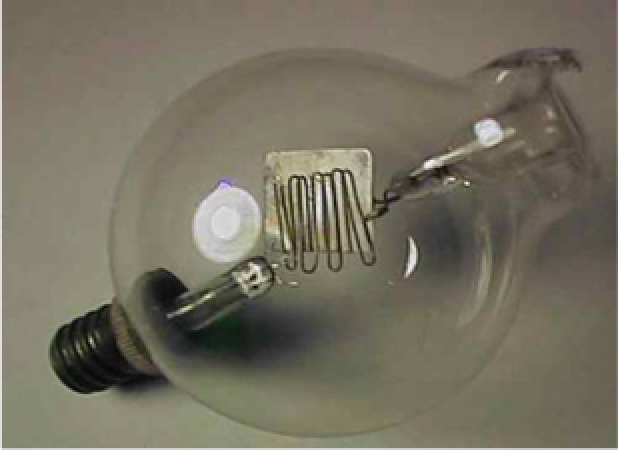
\includegraphics[keepaspectratio]{lec/../images/lec/lec-01-vacuum_tube.png}}

}

\caption{1906 die Elektronenröhre}

\end{figure}%

\begin{figure}[H]

{\centering \pandocbounded{\includegraphics[keepaspectratio]{lec/../images/lec/lec-01-1st_transistor.png}}

}

\caption{1947 der erste Transistor, Bell Labs Foto}

\end{figure}%

\section{Damals und heute}\label{damals-und-heute}

\begin{figure}[H]

{\centering \pandocbounded{\includegraphics[keepaspectratio]{lec/../images/lec/lec-01-1st_ic_kilby.png}}

}

\caption{1958 Jack Kilby's erster IC}

\end{figure}%

\begin{figure}[H]

{\centering \pandocbounded{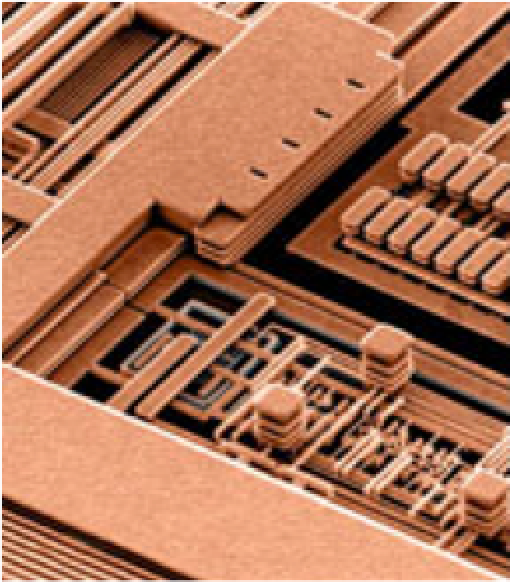
\includegraphics[keepaspectratio]{lec/../images/lec/lec-01-modern_ic.png}}

}

\caption{Moderner IC}

\end{figure}%

\section{Systemhierarchie}\label{systemhierarchie}

\begin{figure}[H]

{\centering \pandocbounded{\includegraphics[keepaspectratio]{lec/../images/lec/lec-01-system_hierarchy.png}}

}

\caption{Funktionsblöcke eines elektronischen Systems}

\end{figure}%

\begin{itemize}
\item
  Nutzen Sie Hierarchien zur Beschreibung komplexer Systeme
\item
  Teile und herrsche
\end{itemize}

\section{Schnittstellen zur
Aussenwelt}\label{schnittstellen-zur-aussenwelt}

\begin{figure}[H]

{\centering \pandocbounded{\includegraphics[keepaspectratio]{lec/../images/lec/lec-01-real_world_interface.png}}

}

\caption{Interfacing}

\end{figure}%

\section{Meeting mit einem System}\label{meeting-mit-einem-system}

\begin{figure}[H]

{\centering \pandocbounded{\includegraphics[keepaspectratio]{lec/../images/lec/lec-01-smartphone.png}}

}

\caption{Drahtloses Kommunikationssystem}

\end{figure}%

\section{System in a Package (SiP)}\label{system-in-a-package-sip}

\begin{figure}[H]

{\centering \pandocbounded{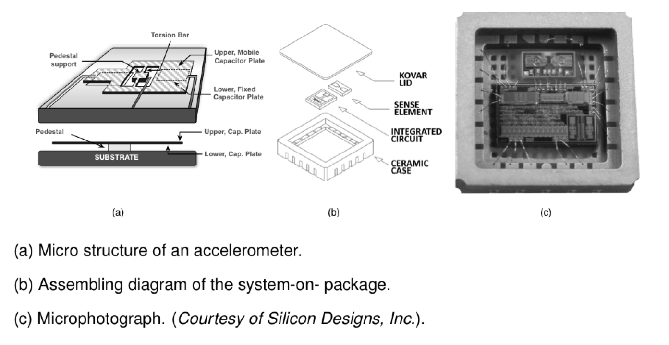
\includegraphics[keepaspectratio]{lec/../images/lec/lec-01-system_in_package.png}}

}

\caption{Beschleunigungssensor}

\end{figure}%

\section{Sie werden unsere Experten}\label{sie-werden-unsere-experten}

\begin{itemize}
\item
  Hintergrundwissen

  \begin{itemize}
  \tightlist
  \item
    Systemverständnis, Architektur, Herstellungsverfahren,
    Implementation
  \end{itemize}
\item
  Unterbewusste Kompetenz

  \begin{itemize}
  \tightlist
  \item
    Abgespeicherte Erfahrungen aus Erfolgsgeschichten und Misserfolgen
  \end{itemize}
\item
  Spezialwissen

  \begin{itemize}
  \tightlist
  \item
    Berufsspezifisches Wissen
  \end{itemize}
\item
  Teamwork Haltung

  \begin{itemize}
  \tightlist
  \item
    Kommunikationsfähigkeit, Berichtswesen und technische Präsentation
  \end{itemize}
\item
  Kreativität
\item
  Tool-Kenntnisse
\end{itemize}

\section{Lernziele des Moduls}\label{lernziele-des-moduls}

\begin{itemize}
\item
  Elektrische Systeme mathematisch und graphisch im Zeit- und
  Frequenzbereich beschreiben
\item
  Netzwerkanalyse mit RLC-Gliedern
\item
  Spezielle Netzwerke, wie Messbrücken, Schwingkreise und ideale
  Transformatoren, dimensionieren.
\end{itemize}

\section{Seminaristischer Unterricht}\label{seminaristischer-unterricht}

\begin{itemize}
\item
  Komplexe Wechselstromrechnung
\item
  Diskrete Bauelemente und ihre Modellierung (RLC)
\item
  Methodik der Netzwerkanalyse
\item
  Anwendungsbeispiele mit EDA-Werkzeugen und wissenschaftliches Rechnen
  (Scientific Computing)
\end{itemize}

\section{Beschreibung elektrotechnischer
Systeme}\label{beschreibung-elektrotechnischer-systeme}

\begin{itemize}
\item
  verschiedene Stufen der Vereinfachung
\item
  Felder / Wellen / Optik / HF-Technik

  \begin{itemize}
  \tightlist
  \item
    Maxwell-Gleichungen \begin{align}
    \oint \mathbf{H} d\mathbf{s} &= \iint \mathbf{J} + \dot{D} d\mathbf{A} \\
    \oint \mathbf{E} d\mathbf{s} &= - \iint \dot{B} d\mathbf{A}
    \end{align}
  \end{itemize}
\item
  bei lokaler Konzentration der Feldenergie \(\Rightarrow\)
  quasi-statische Näherung
\item
  Mikrowellentechnik / Leitungstechnik

  \begin{itemize}
  \item
    verteilte Schaltungen \(l\), \(c\), \(\rho\)
  \item
    Kopplung, Laufzeit \(\tau = a/v\)
  \end{itemize}
\item
  \emph{kleine} Systeme mit \(a << \lambda\) bzw. \emph{kurze}
  Laufzeiten mit \(\tau << T\)
\item
  Regelungstechnik / Impulstechnik

  \begin{itemize}
  \item
    Ersatzschaltungen
  \item
    (Block-)Schaltbilder
  \end{itemize}
\item
  eingeschwungener Zustand
\item
  NF-Technik

  \begin{itemize}
  \tightlist
  \item
    stationär-periodische Signale
  \end{itemize}
\item
  Sinussignale
\item
  Energietechnik

  \begin{itemize}
  \tightlist
  \item
    monofrequente Signale \(U = Z \cdot I\)
  \end{itemize}
\item
  Frequenz \(f \rightarrow 0\)
\item
  Gleichstromtechnik

  \begin{itemize}
  \tightlist
  \item
    Ohmsches Gesetz \(U = R \cdot I\)
  \end{itemize}
\end{itemize}

\section{Konzentrierte
Schaltelemente}\label{konzentrierte-schaltelemente}

\begin{tcolorbox}[enhanced jigsaw, arc=.35mm, opacityback=0, opacitybacktitle=0.6, left=2mm, breakable, title=\textcolor{quarto-callout-note-color}{\faInfo}\hspace{0.5em}{Stromdichte}, bottomrule=.15mm, toptitle=1mm, rightrule=.15mm, titlerule=0mm, leftrule=.75mm, colframe=quarto-callout-note-color-frame, colbacktitle=quarto-callout-note-color!10!white, bottomtitle=1mm, colback=white, toprule=.15mm, coltitle=black]

\[
\frac{\int E(r,t) ds}{\iint J(r,t) dA} = \frac{u(t)}{i(t)} \Rightarrow R
\]

\end{tcolorbox}

\begin{tcolorbox}[enhanced jigsaw, arc=.35mm, opacityback=0, opacitybacktitle=0.6, left=2mm, breakable, title=\textcolor{quarto-callout-note-color}{\faInfo}\hspace{0.5em}{Verschiebungsdichte}, bottomrule=.15mm, toptitle=1mm, rightrule=.15mm, titlerule=0mm, leftrule=.75mm, colframe=quarto-callout-note-color-frame, colbacktitle=quarto-callout-note-color!10!white, bottomtitle=1mm, colback=white, toprule=.15mm, coltitle=black]

\[
\frac{\iint D(r,t) dA}{\int E(r,t) ds} = \frac{q(t)}{u(t)} \Rightarrow C
\]

\end{tcolorbox}

\begin{tcolorbox}[enhanced jigsaw, arc=.35mm, opacityback=0, opacitybacktitle=0.6, left=2mm, breakable, title=\textcolor{quarto-callout-note-color}{\faInfo}\hspace{0.5em}{Flußdichte}, bottomrule=.15mm, toptitle=1mm, rightrule=.15mm, titlerule=0mm, leftrule=.75mm, colframe=quarto-callout-note-color-frame, colbacktitle=quarto-callout-note-color!10!white, bottomtitle=1mm, colback=white, toprule=.15mm, coltitle=black]

\[
\frac{\iint B(r,t) dA}{\oint H(r,t) ds} = \frac{u(t)}{i(t)} \Rightarrow L
\]

\end{tcolorbox}

\section{Harmonische Signale \ldots{}}\label{harmonische-signale}

\begin{tcolorbox}[enhanced jigsaw, arc=.35mm, opacityback=0, opacitybacktitle=0.6, left=2mm, breakable, title=\textcolor{quarto-callout-note-color}{\faInfo}\hspace{0.5em}{als Zeitfunktion}, bottomrule=.15mm, toptitle=1mm, rightrule=.15mm, titlerule=0mm, leftrule=.75mm, colframe=quarto-callout-note-color-frame, colbacktitle=quarto-callout-note-color!10!white, bottomtitle=1mm, colback=white, toprule=.15mm, coltitle=black]

\[
u(t) = \hat{U} \cos(\omega t + \phi)
\]

\end{tcolorbox}

\begin{tcolorbox}[enhanced jigsaw, arc=.35mm, opacityback=0, opacitybacktitle=0.6, left=2mm, breakable, title=\textcolor{quarto-callout-note-color}{\faInfo}\hspace{0.5em}{als Zeiger / komplexe Grösse (Phasor)}, bottomrule=.15mm, toptitle=1mm, rightrule=.15mm, titlerule=0mm, leftrule=.75mm, colframe=quarto-callout-note-color-frame, colbacktitle=quarto-callout-note-color!10!white, bottomtitle=1mm, colback=white, toprule=.15mm, coltitle=black]

\[
U = \lvert \hat{U} \lvert e^{j \phi}
\]

\end{tcolorbox}

\chapter{Netzwerkerregung}\label{netzwerkerregung}

\section{Schaltzeichen}\label{schaltzeichen}

``In Deutschland sind elektrische Schaltzeichen durch DIN EN 60617
Graphische Symbole für Schaltpläne bzw. IEC 60617 genormt. Sie ersetzen
seit 1996--1998 die DIN 40700 / DIN 40900.''

\href{https://de.wikipedia.org/wiki/Liste_der_Schaltzeichen_\%28Elektrik/Elektronik\%29\#Ideale_Stromkreise}{Schaltzeichen
nach DIN EN 60617}

\section{Erregungsarten}\label{erregungsarten}

\begin{itemize}
\item
  Gleichvorgänge
\item
  Nichtperiodische Vorgänge
\item
  Periodische Vorgänge, Spezialfall sind harmonische (sinus-,
  kosinusförmige) Vorgänge mit der Periodendauer \(T\)
\item
  Gleichgrößen mit \(f(t)\) = const. werden mit großen lateinischen
  Buchstaben gekennzeichnet, Gleichspannung \(U\) und Gleichstrom \(I\)
\item
  Zeitveränderliche Größen, hierbei ändert die Erregergröße \(f(t)\)
  ihre Amplitude und/oder ihre Richtung zeitlich. Der Wert von \(f(t)\)
  zum momentanen Zeitpunkt heißt Augenblicks- oder Momentanwert \(f(t)\)
  der physikalischen Größe. Momentanwerte erhalten kleine lateinische
  Buchstaben, Spannung \(u\) und Strom \(i\).
\end{itemize}

\section{Sinusförmige Erregung, periodische
Vorgänge}\label{sinusfuxf6rmige-erregung-periodische-vorguxe4nge}

(Wikipedia 2025) (Wikipedia 2024b)

\begin{tcolorbox}[enhanced jigsaw, arc=.35mm, opacityback=0, opacitybacktitle=0.6, left=2mm, breakable, title=\textcolor{quarto-callout-note-color}{\faInfo}\hspace{0.5em}{Definitionen}, bottomrule=.15mm, toptitle=1mm, rightrule=.15mm, titlerule=0mm, leftrule=.75mm, colframe=quarto-callout-note-color-frame, colbacktitle=quarto-callout-note-color!10!white, bottomtitle=1mm, colback=white, toprule=.15mm, coltitle=black]

\begin{itemize}
\item
  \(f(t)=f(t+nT)\) mit \(n=0, 1 ...\)
\item
  Frequenz \(f=1/T\)
\item
  Kreisfrequenz \(\omega=2\pi f = 2\pi/T\)
\item
  Periodendauer \(T\)
\item
  Wechselgröße allgem.
  \(a(t)=\hat{A} \sin (\omega t +\varphi) = \hat{A} \sin(\omega t + \omega t_0)\)
\item
  Scheitelwert, Maximalwert der Amplitude \(\hat{A}=\max{A}=A_{max}\)
\item
  Nullphasenwinkel bzw. Nullzeitpunkt \(\varphi=\omega t_0\)
\item
  Erregergröße wird aufgetragen mit \(\omega t\) und nicht \(t\);
  \(\psi(t) = \omega t + \varphi = \omega t + \omega t_0\)
\item
  Bogenmaß \(\psi/\mbox{Bogenmaß} = \frac{2 \pi}{360} \psi/\mbox{Grad}\)
\end{itemize}

\end{tcolorbox}

\section{Eigenschaften harmonischer
Funktionen}\label{eigenschaften-harmonischer-funktionen}

\begin{itemize}
\item
  Differentiation, Integration und Addition, Subtraktion mithilfe von
  Additionstheoremen
\item
  Aufspaltung einer harmonischen Schwingung und Koeffizientenvergleich
\end{itemize}

\begin{tcolorbox}[enhanced jigsaw, arc=.35mm, opacityback=0, opacitybacktitle=0.6, left=2mm, breakable, title=\textcolor{quarto-callout-note-color}{\faInfo}\hspace{0.5em}{Zusammengefasst}, bottomrule=.15mm, toptitle=1mm, rightrule=.15mm, titlerule=0mm, leftrule=.75mm, colframe=quarto-callout-note-color-frame, colbacktitle=quarto-callout-note-color!10!white, bottomtitle=1mm, colback=white, toprule=.15mm, coltitle=black]

Bei Addition, Differentiation und Integration von harmonischen
Funktionen der Kreisfrequenz \(\omega\) entstehen wieder harmonische
Funktionen der gleichen Frequenz, aber veränderter Amplitude und Phase.
Bei der Überlagerung zweier harmonischer Größen mit verschiedener
Frequenz entsteht zwar eine periodische Schwingung, aber keine
Sinusschwingung (harmonische).

\end{tcolorbox}

\section{Mittelwerte periodischer
Zeitfunktionen}\label{mittelwerte-periodischer-zeitfunktionen}

\begin{tcolorbox}[enhanced jigsaw, arc=.35mm, opacityback=0, opacitybacktitle=0.6, left=2mm, breakable, title=\textcolor{quarto-callout-note-color}{\faInfo}\hspace{0.5em}{Arithmetischer Mittelwert - linearer Mittelwert - Gleichwert}, bottomrule=.15mm, toptitle=1mm, rightrule=.15mm, titlerule=0mm, leftrule=.75mm, colframe=quarto-callout-note-color-frame, colbacktitle=quarto-callout-note-color!10!white, bottomtitle=1mm, colback=white, toprule=.15mm, coltitle=black]

\begin{align}
\overline{u(t)} &= \frac{1}{T} \int_t^{t+T} u(\tau) \mathrm{d} \tau
\end{align}

\end{tcolorbox}

\begin{tcolorbox}[enhanced jigsaw, arc=.35mm, opacityback=0, opacitybacktitle=0.6, left=2mm, breakable, title=\textcolor{quarto-callout-note-color}{\faInfo}\hspace{0.5em}{Gleichrichtmittelwert}, bottomrule=.15mm, toptitle=1mm, rightrule=.15mm, titlerule=0mm, leftrule=.75mm, colframe=quarto-callout-note-color-frame, colbacktitle=quarto-callout-note-color!10!white, bottomtitle=1mm, colback=white, toprule=.15mm, coltitle=black]

\begin{align}
\overline{\lvert u(t) \lvert} &= \frac{1}{T} \int_t^{t+T} \lvert u(\tau) \lvert \mathrm{d} \tau
\end{align}

\end{tcolorbox}

\begin{tcolorbox}[enhanced jigsaw, arc=.35mm, opacityback=0, opacitybacktitle=0.6, left=2mm, breakable, title=\textcolor{quarto-callout-note-color}{\faInfo}\hspace{0.5em}{Quadratischer Mittelwert - Effektivwert}, bottomrule=.15mm, toptitle=1mm, rightrule=.15mm, titlerule=0mm, leftrule=.75mm, colframe=quarto-callout-note-color-frame, colbacktitle=quarto-callout-note-color!10!white, bottomtitle=1mm, colback=white, toprule=.15mm, coltitle=black]

\begin{align}
U_{eff} = \sqrt{\overline{u^2(t)}} &= \sqrt{\frac{1}{T} \int_t^{t+T} u^2(\tau) \mathrm{d} \tau}
\end{align}

\end{tcolorbox}

\section{\texorpdfstring{\(u/i\)-Verhalten}{u/i-Verhalten}}\label{ui-verhalten}

\begin{tcolorbox}[enhanced jigsaw, arc=.35mm, opacityback=0, opacitybacktitle=0.6, left=2mm, breakable, title=\textcolor{quarto-callout-note-color}{\faInfo}\hspace{0.5em}{Widerstand \(R\) - Einheit: 1 \(\Omega\)}, bottomrule=.15mm, toptitle=1mm, rightrule=.15mm, titlerule=0mm, leftrule=.75mm, colframe=quarto-callout-note-color-frame, colbacktitle=quarto-callout-note-color!10!white, bottomtitle=1mm, colback=white, toprule=.15mm, coltitle=black]

\begin{align}
u(t) &= R \cdot i(t) \\
&= R \cdot \hat{I} \sin(\omega t + \varphi_i) \\
&= \hat{U} \sin(\omega t + \varphi_u)
\end{align}

\end{tcolorbox}

\begin{tcolorbox}[enhanced jigsaw, arc=.35mm, opacityback=0, opacitybacktitle=0.6, left=2mm, breakable, title=\textcolor{quarto-callout-note-color}{\faInfo}\hspace{0.5em}{Induktivität \(L\) - Einheit: 1 H = 1 Vs/A}, bottomrule=.15mm, toptitle=1mm, rightrule=.15mm, titlerule=0mm, leftrule=.75mm, colframe=quarto-callout-note-color-frame, colbacktitle=quarto-callout-note-color!10!white, bottomtitle=1mm, colback=white, toprule=.15mm, coltitle=black]

\begin{align}
u(t) &= L \cdot \frac{di_L(t)}{dt} \\
&= \omega L \cdot \hat{I} \cos(\omega t + \varphi_i) \\
&= \omega L \hat{I} \sin(\omega t + \varphi_i + \frac{\pi}{2})
\end{align}

\end{tcolorbox}

\begin{tcolorbox}[enhanced jigsaw, arc=.35mm, opacityback=0, opacitybacktitle=0.6, left=2mm, breakable, title=\textcolor{quarto-callout-note-color}{\faInfo}\hspace{0.5em}{Kapazität \(C\) - Einheit: 1 F = 1 C/V = 1 As/V}, bottomrule=.15mm, toptitle=1mm, rightrule=.15mm, titlerule=0mm, leftrule=.75mm, colframe=quarto-callout-note-color-frame, colbacktitle=quarto-callout-note-color!10!white, bottomtitle=1mm, colback=white, toprule=.15mm, coltitle=black]

\begin{align}
i(t) &= C \cdot \frac{du_C(t)}{dt} \\
&= \omega C \cdot \hat{U} \cos(\omega t + \varphi_u) \\
&= \omega C \hat{U} \sin(\omega t + \varphi_u + \frac{\pi}{2})
\end{align}

\end{tcolorbox}

\chapter{Komplexe
Wechselstromrechnung}\label{komplexe-wechselstromrechnung}

\section{Beschreibung und Analyse im
Frequenzbereich}\label{beschreibung-und-analyse-im-frequenzbereich}

\begin{tcolorbox}[enhanced jigsaw, arc=.35mm, opacityback=0, opacitybacktitle=0.6, left=2mm, breakable, title=\textcolor{quarto-callout-note-color}{\faInfo}\hspace{0.5em}{Problemstellung}, bottomrule=.15mm, toptitle=1mm, rightrule=.15mm, titlerule=0mm, leftrule=.75mm, colframe=quarto-callout-note-color-frame, colbacktitle=quarto-callout-note-color!10!white, bottomtitle=1mm, colback=white, toprule=.15mm, coltitle=black]

Bei zukünftigen Schaltungen ist es nicht mehr möglich, direkt mit den
Zeitfunktionen für Spannungen und Ströme zu arbeiten.

Die von den Gleichstromnetzen bekannten Lösungsverfahren aus dem ersten
Semester, die von linearen algebraischen Gleichungssystemen ausgehen
(Maschen-, Knoten- und andere Verfahren) können nicht übernommen werden.

\end{tcolorbox}

\begin{tcolorbox}[enhanced jigsaw, arc=.35mm, opacityback=0, opacitybacktitle=0.6, left=2mm, breakable, title=\textcolor{quarto-callout-note-color}{\faInfo}\hspace{0.5em}{Symbolische Verfahren/Methoden}, bottomrule=.15mm, toptitle=1mm, rightrule=.15mm, titlerule=0mm, leftrule=.75mm, colframe=quarto-callout-note-color-frame, colbacktitle=quarto-callout-note-color!10!white, bottomtitle=1mm, colback=white, toprule=.15mm, coltitle=black]

\begin{itemize}
\item
  komplexe Darstellung (analytisches Verfahren)
\item
  Zeigerdarstellung (graphisches Verfahren)
\item
  Wechselstromanalyse
\item
  Betrachtungen beruhen auf der Verwendung sinusförmiger Eingangsgrößen
\item
  Zeitbereich ist physikalische Realität mit gew. und partiellen
  Differentialgleichung (ODE, PDE)
\item
  Frequenzbereich hat mathematisch-formale Bedeutung
\end{itemize}

\end{tcolorbox}

\section{Symbolisches Verfahren}\label{symbolisches-verfahren}

\begin{itemize}
\item
  Man ordnet nach einer gewissen Regel jeder Sinusgröße eine symbolische
  Größe zu (z.B. einen Vektor oder eine komplexe Zahl);
\item
  Man schreibt die Differentialgleichungen des Netzwerkes mit den
  symbolischen Größen;
\item
  Statt die Differentialgleichungen zu lösen, löst man die Gleichungen
  für die Symbole und bestimmt die unbekannten Größen.
\item
  Man transformiert die gefundenen Symbolgrößen zurück in die gesuchten
  Sinusgrößen.
\item
  entn. (Marinescu und Marinescu 2016)
\end{itemize}

\section{Vorteile des
Frequenzbereichs}\label{vorteile-des-frequenzbereichs}

\begin{itemize}
\item
  zeitl. Differentiation und Integration geht über in Multiplikation und
  Division mit dem Differentialoperator \(s=\sigma+j\omega\) (komplexe
  Frequenz); häufig genügt es sich auf die imaginäre Frequenz
  \(s=j \omega\) zu beschränken.
\item
  u-i-Zusammenhänge des Zeitbereichs \(\rightarrow\) ohmsche Form im
  Frequenzbereich durch komplexen Widerstands-/Leitwertbegriff
\item
  ODE's gehen über in algebraische Gleichungen
\item
  gleichwertige Darstellung harmonischer Funktionen durch komplexe
  Größen \(\rightarrow\) Zeiger
\end{itemize}

\section{Funktionaltransformation}\label{funktionaltransformation}

\begin{tcolorbox}[enhanced jigsaw, arc=.35mm, opacityback=0, opacitybacktitle=0.6, left=2mm, breakable, title=\textcolor{quarto-callout-note-color}{\faInfo}\hspace{0.5em}{Euler'sche Formel}, bottomrule=.15mm, toptitle=1mm, rightrule=.15mm, titlerule=0mm, leftrule=.75mm, colframe=quarto-callout-note-color-frame, colbacktitle=quarto-callout-note-color!10!white, bottomtitle=1mm, colback=white, toprule=.15mm, coltitle=black]

\[
\sigma + j \omega = a e^{j \varphi} = a \left( \cos(\varphi) + j \sin(\varphi) \right) 
\]

\[
a = \sqrt{\sigma^2 + \omega^2} \quad \mbox{und} \quad \varphi = \arctan\left(\frac{\omega}{\sigma}\right)
\]

\end{tcolorbox}

\begin{tcolorbox}[enhanced jigsaw, arc=.35mm, opacityback=0, opacitybacktitle=0.6, left=2mm, breakable, title=\textcolor{quarto-callout-note-color}{\faInfo}\hspace{0.5em}{Exponentialdarstellung}, bottomrule=.15mm, toptitle=1mm, rightrule=.15mm, titlerule=0mm, leftrule=.75mm, colframe=quarto-callout-note-color-frame, colbacktitle=quarto-callout-note-color!10!white, bottomtitle=1mm, colback=white, toprule=.15mm, coltitle=black]

\begin{align}
\cos(n\omega t) &= \frac{1}{2}\left( e^{j n \omega t} + e^{-jn\omega t}\right), \quad n=0, 1, \ldots \\
\sin(n\omega t) &= \frac{1}{j2}\left( e^{j n \omega t} - e^{-jn\omega t}\right), \quad n=0, 1, \ldots
\end{align}

\end{tcolorbox}

\begin{tcolorbox}[enhanced jigsaw, arc=.35mm, opacityback=0, opacitybacktitle=0.6, left=2mm, breakable, title=\textcolor{quarto-callout-note-color}{\faInfo}\hspace{0.5em}{Transformation}, bottomrule=.15mm, toptitle=1mm, rightrule=.15mm, titlerule=0mm, leftrule=.75mm, colframe=quarto-callout-note-color-frame, colbacktitle=quarto-callout-note-color!10!white, bottomtitle=1mm, colback=white, toprule=.15mm, coltitle=black]

\begin{align}
f(t) &= \hat{A}\cos(\omega t + \varphi_a) \\
&= \frac{1}{2} \underbrace{\hat{A} e^{j \varphi_a}}_{Phasor} e^{j \omega t} 
+ \frac{1}{2} \underbrace{\hat{A} e^{-j\varphi_a}}_{Phasor} e^{-j \omega t} \\ 
&= \frac{1}{2}\underline{\hat{A}} e^{j \omega t} + \frac{1}{2}\underline{\hat{A}}^{*} e^{-j \omega t} \\
&= \mathfrak{Re}\left\{\underline{\hat{A}}e^{j\omega t}\right\} \\
&= \mathfrak{Re}\left\{\hat{A}e^{j \varphi_a}e^{j \omega t}\right\} \\ 
&= \mathfrak{Re}\left\{\hat{A}\left( \cos(\omega t + \varphi_a) + j \sin(\omega t + \varphi_a)\right)\right\}
\end{align}

\end{tcolorbox}

\subsection{Definitionen}\label{definitionen-1}

\begin{tcolorbox}[enhanced jigsaw, arc=.35mm, opacityback=0, opacitybacktitle=0.6, left=2mm, breakable, title=\textcolor{quarto-callout-note-color}{\faInfo}\hspace{0.5em}{rotierender Zeiger, komplexer Momentanwert}, bottomrule=.15mm, toptitle=1mm, rightrule=.15mm, titlerule=0mm, leftrule=.75mm, colframe=quarto-callout-note-color-frame, colbacktitle=quarto-callout-note-color!10!white, bottomtitle=1mm, colback=white, toprule=.15mm, coltitle=black]

\[
\underline{f}(t) = \underline{\hat{A}} e^{j\omega t} = \hat{A} e^{j \varphi_a} e^{j \omega t}
\]

\end{tcolorbox}

\begin{tcolorbox}[enhanced jigsaw, arc=.35mm, opacityback=0, opacitybacktitle=0.6, left=2mm, breakable, title=\textcolor{quarto-callout-note-color}{\faInfo}\hspace{0.5em}{ruhender Zeiger, komplexer Scheitelwert, Phasor}, bottomrule=.15mm, toptitle=1mm, rightrule=.15mm, titlerule=0mm, leftrule=.75mm, colframe=quarto-callout-note-color-frame, colbacktitle=quarto-callout-note-color!10!white, bottomtitle=1mm, colback=white, toprule=.15mm, coltitle=black]

\[
\underline{f}(0) = \underline{\hat{A}} = \hat{A} e^{j\varphi_a}
\]

\end{tcolorbox}

\begin{tcolorbox}[enhanced jigsaw, arc=.35mm, opacityback=0, opacitybacktitle=0.6, left=2mm, breakable, title=\textcolor{quarto-callout-note-color}{\faInfo}\hspace{0.5em}{komplexer Effektivwert}, bottomrule=.15mm, toptitle=1mm, rightrule=.15mm, titlerule=0mm, leftrule=.75mm, colframe=quarto-callout-note-color-frame, colbacktitle=quarto-callout-note-color!10!white, bottomtitle=1mm, colback=white, toprule=.15mm, coltitle=black]

\[
\underline{A} = \frac{1}{\sqrt{2}} \hat{A} e^{j \varphi_a}
\]

\end{tcolorbox}

\section{Zeigerdarstellung}\label{zeigerdarstellung}

\begin{figure}

\centering{

\includegraphics[width=4.16667in,height=\textheight,keepaspectratio]{lec/../images/lec/phasor-diagram.pdf}

}

\caption{\label{fig-phasor}Phasor-Diagramm}

\end{figure}%

\subsection{Grundschaltelemente}\label{grundschaltelemente}

\begin{itemize}
\item
  Sinusgröße \(i(t) = I \sqrt{2} \sin(\omega t + \varphi)\)
\item
  da alle in einer Schaltung vorkommenen Sinusgrößen (meist) dieselbe
  Kreisfrequenz \(\omega\) aufweisen, kann man diese außer Acht lassen
  und die Zeiger als stehend betrachten;
\item
  Der Faktor 2 in den Scheitelwerten aller Sinusgrößen wird nicht
  berücksichtigt und man arbeitet mit Effektivwerten, {[}\ldots{]}, vor
  allem zur Bestimmung von Leistungen. Man reduziert also die
  Zeigerlängen im Maßstab \(\frac{1}{\sqrt{2}}\).
\end{itemize}

\subsection{Komplexe Zahlen}\label{komplexe-zahlen}

\begin{itemize}
\tightlist
\item
  Eingabe als Literal
\end{itemize}

\begin{Shaded}
\begin{Highlighting}[]
\NormalTok{z }\OperatorTok{=} \DecValTok{3} \OperatorTok{+} \OtherTok{2j}
\end{Highlighting}
\end{Shaded}

\begin{itemize}
\tightlist
\item
  Eingabe als Funktion
\end{itemize}

\begin{Shaded}
\begin{Highlighting}[]
\NormalTok{z }\OperatorTok{=} \BuiltInTok{complex}\NormalTok{(}\DecValTok{3}\NormalTok{, }\DecValTok{2}\NormalTok{)}
\end{Highlighting}
\end{Shaded}

\begin{itemize}
\tightlist
\item
  Für mathematische Operationen benötigt man eine Bibliothek:
\end{itemize}

\begin{Shaded}
\begin{Highlighting}[]
\ImportTok{import}\NormalTok{ cmath, math, numpy}

\NormalTok{z }\OperatorTok{=} \DecValTok{4} \OperatorTok{+} \OtherTok{4j}
\end{Highlighting}
\end{Shaded}

\subsection{Berechnung von Betrag und
Phase}\label{berechnung-von-betrag-und-phase}

\begin{Shaded}
\begin{Highlighting}[]
\NormalTok{z\_abs }\OperatorTok{=} \BuiltInTok{abs}\NormalTok{(z) }
\NormalTok{z\_ph }\OperatorTok{=}\NormalTok{ cmath.phase(z)}
\BuiltInTok{print}\NormalTok{(}\StringTok{\textquotesingle{}Betrag =\textquotesingle{}}\NormalTok{, z\_abs)}
\BuiltInTok{print}\NormalTok{(}\StringTok{\textquotesingle{}Phase in rad =\textquotesingle{}}\NormalTok{, z\_ph)}
\BuiltInTok{print}\NormalTok{(}\StringTok{\textquotesingle{}Phase in Grad =\textquotesingle{}}\NormalTok{, numpy.degrees(z\_ph))}
\end{Highlighting}
\end{Shaded}

\begin{verbatim}
Betrag = 5.656854249492381
Phase in rad = 0.7853981633974483
Phase in Grad = 45.0
\end{verbatim}

\subsection{Darstellung in der komplexen
Ebene}\label{darstellung-in-der-komplexen-ebene}

\begin{Shaded}
\begin{Highlighting}[]
\ImportTok{import}\NormalTok{ matplotlib.pyplot }\ImportTok{as}\NormalTok{ plt}

\NormalTok{plt.plot(z.real, z.imag, }\StringTok{\textquotesingle{}x\textquotesingle{}}\NormalTok{)}
\end{Highlighting}
\end{Shaded}

\pandocbounded{
\includegraphics[keepaspectratio]{lec/lec_03_files/figure-pdf/cell-6-output-1.png}}

\subsection{Kartesische Form}\label{kartesische-form}

\subsection{Polare Form}\label{polare-form}

\subsection{Kartesisch \textless-\textgreater{}
Polar}\label{kartesisch---polar}

\subsection{Euler's Formel}\label{eulers-formel}

\subsection{Euler's inverse Formel}\label{eulers-inverse-formel}

\subsection{Algebraische Regeln}\label{algebraische-regeln}

\chapter{Impedanz, Admittanz und
Leistung}\label{impedanz-admittanz-und-leistung}

\section{Widerstandsoperator}\label{widerstandsoperator}

\begin{tcolorbox}[enhanced jigsaw, arc=.35mm, opacityback=0, opacitybacktitle=0.6, left=2mm, breakable, title=\textcolor{quarto-callout-note-color}{\faInfo}\hspace{0.5em}{u/i-Verhalten}, bottomrule=.15mm, toptitle=1mm, rightrule=.15mm, titlerule=0mm, leftrule=.75mm, colframe=quarto-callout-note-color-frame, colbacktitle=quarto-callout-note-color!10!white, bottomtitle=1mm, colback=white, toprule=.15mm, coltitle=black]

\[
\frac{\underline{u}(t)}{\underline{i}(t)} = \frac{\underline{\hat{U}}e^{j \omega t}}{\underline{\hat{I}}e^{j \omega t}}
= \frac{\hat{U}}{\hat{I}} e^{j(\varphi_u \varphi_i)} = \underline{Z} 
\]

\end{tcolorbox}

\begin{tcolorbox}[enhanced jigsaw, arc=.35mm, opacityback=0, opacitybacktitle=0.6, left=2mm, breakable, title=\textcolor{quarto-callout-note-color}{\faInfo}\hspace{0.5em}{Impedanz}, bottomrule=.15mm, toptitle=1mm, rightrule=.15mm, titlerule=0mm, leftrule=.75mm, colframe=quarto-callout-note-color-frame, colbacktitle=quarto-callout-note-color!10!white, bottomtitle=1mm, colback=white, toprule=.15mm, coltitle=black]

\begin{align}
\underline{Z} &= \frac{\underline{u}(t)}{\underline{i}(t)} =
\frac{\underline{\hat{U}}e^{j \omega t}}{\underline{\hat{I}}e^{j \omega t}} =
\frac{\hat{U}}{\hat{I}}e^{\varphi_u-\varphi_i} \\
&= Z e^{j \varphi_z} = Z \left( \cos(\varphi_z) + j \sin(\varphi_z) \right) \\
&= \operatorname{Re}{\underline{Z}} + j \operatorname{Im}{\underline{Z}} \\
&= R + j X
\end{align}

\end{tcolorbox}

\begin{tcolorbox}[enhanced jigsaw, arc=.35mm, opacityback=0, opacitybacktitle=0.6, left=2mm, breakable, title=\textcolor{quarto-callout-note-color}{\faInfo}\hspace{0.5em}{Eigenschaften}, bottomrule=.15mm, toptitle=1mm, rightrule=.15mm, titlerule=0mm, leftrule=.75mm, colframe=quarto-callout-note-color-frame, colbacktitle=quarto-callout-note-color!10!white, bottomtitle=1mm, colback=white, toprule=.15mm, coltitle=black]

\begin{align}
Z &= \lvert\underline{Z}\lvert = \sqrt{R^2 + X^2} & &\mbox{Scheinwiderstand} \\
R &= \operatorname{Re}{\underline{Z}} & &\mbox{Wirkwiderstand (Resistanz)} \\
X &= \operatorname{Im}{\underline{Z}} & &\mbox{Blindwiderstand (Reaktanz)} \\
\tan(\varphi_z) &= \frac{\operatorname{Im}{\underline{Z}}}{\operatorname{Re}{\underline{Z}}} = \frac{X_r}{R_r}  & & \\
\varphi_z &= \varphi_u - \varphi_i = \arctan\left(\frac{X_r}{R_r}\right) & &
\end{align}

\end{tcolorbox}

\section{Leitwertoperator}\label{leitwertoperator}

\begin{tcolorbox}[enhanced jigsaw, arc=.35mm, opacityback=0, opacitybacktitle=0.6, left=2mm, breakable, title=\textcolor{quarto-callout-note-color}{\faInfo}\hspace{0.5em}{Harmonische Anregung}, bottomrule=.15mm, toptitle=1mm, rightrule=.15mm, titlerule=0mm, leftrule=.75mm, colframe=quarto-callout-note-color-frame, colbacktitle=quarto-callout-note-color!10!white, bottomtitle=1mm, colback=white, toprule=.15mm, coltitle=black]

\begin{align}
u(t) &= \hat{U} \cos(\omega t + \varphi_u) & \underline{u}(t) &= \underline{\hat{U}} e^{j \omega t} \\
i(t) &= \hat{I} \cos(\omega t + \varphi_i) & \underline{i}(t) &= \underline{\hat{I}} e^{j \omega t}
\end{align}

\end{tcolorbox}

\begin{tcolorbox}[enhanced jigsaw, arc=.35mm, opacityback=0, opacitybacktitle=0.6, left=2mm, breakable, title=\textcolor{quarto-callout-note-color}{\faInfo}\hspace{0.5em}{Admittanz}, bottomrule=.15mm, toptitle=1mm, rightrule=.15mm, titlerule=0mm, leftrule=.75mm, colframe=quarto-callout-note-color-frame, colbacktitle=quarto-callout-note-color!10!white, bottomtitle=1mm, colback=white, toprule=.15mm, coltitle=black]

\begin{align}
\underline{Y} &= \frac{\underline{i}(t)}{\underline{u}(t)} =
\frac{\underline{\hat{I}}e^{j \omega t}}{\underline{\hat{U}}e^{j \omega t}} =
\frac{\hat{I}}{\hat{U}}e^{\varphi_i-\varphi_u} \\
&= Y e^{j \varphi_y} = Y \left( \cos(\varphi_y) + j \sin(\varphi_y) \right) \\
&= \operatorname{Re}{\underline{Y}} + j \operatorname{Im}{\underline{Y}} \\
&= G + j B
\end{align}

\end{tcolorbox}

\begin{tcolorbox}[enhanced jigsaw, arc=.35mm, opacityback=0, opacitybacktitle=0.6, left=2mm, breakable, title=\textcolor{quarto-callout-note-color}{\faInfo}\hspace{0.5em}{Eigenschaften}, bottomrule=.15mm, toptitle=1mm, rightrule=.15mm, titlerule=0mm, leftrule=.75mm, colframe=quarto-callout-note-color-frame, colbacktitle=quarto-callout-note-color!10!white, bottomtitle=1mm, colback=white, toprule=.15mm, coltitle=black]

\begin{align}
Y &= \lvert\underline{Y}\lvert = \sqrt{G^2 + B^2} & &\mbox{Scheinleitwert} \\
G &= \operatorname{Re}{\underline{Y}} & &\mbox{Wirkleitwert (Konduktanz)} \\
B &= \operatorname{Im}{\underline{Y}} & &\mbox{Blindleitwert (Suszeptanz)} \\
\tan(\varphi_y) &= \frac{\operatorname{Im}{\underline{Y}}}{\operatorname{Re}{\underline{Y}}} = \frac{B}{G}  & & \\
\varphi_y &= \varphi_i - \varphi_u = \arctan\left(\frac{B}{G}\right) & &
\end{align}

\end{tcolorbox}

\section{Vergleich von
RLC-Netzwerken}\label{vergleich-von-rlc-netzwerken}

\begin{align}
\mbox{Zeitbereich} &: & u &= i R &  u &= \frac{1}{C} \int i\, dt & u &= L \frac{di}{dt} \\
\mbox{Frequenzbereich} &: & \underline{u} &= \underline{i} R &
\underline{u} &= \frac{1}{j \omega C} \underline{i} &
\underline{u} &= j \omega L \underline{i} \\
\mbox{Impedanz} &: & \underline{Z} &= R &
\underline{Z} &= j X_C = -\frac{j}{\omega C} &
\underline{Z} &= j X_L = j \omega L \\
\mbox{Phase} &: & \varphi_Z&= 0 & \varphi_Z &= -\frac{\pi}{2} & \varphi_Z &= \frac{\pi}{2}
\end{align}

\section{Leistung von
Wechselsignalen}\label{leistung-von-wechselsignalen}

\begin{tcolorbox}[enhanced jigsaw, arc=.35mm, opacityback=0, opacitybacktitle=0.6, left=2mm, breakable, title=\textcolor{quarto-callout-note-color}{\faInfo}\hspace{0.5em}{Harmonische Anregung}, bottomrule=.15mm, toptitle=1mm, rightrule=.15mm, titlerule=0mm, leftrule=.75mm, colframe=quarto-callout-note-color-frame, colbacktitle=quarto-callout-note-color!10!white, bottomtitle=1mm, colback=white, toprule=.15mm, coltitle=black]

\begin{align}
u(t) &= \hat{U} \cos(\omega t + \varphi_u) & i(t) &= \hat{I} \cos(\omega t + \varphi_i) \\
&= \frac{1}{2} \left( \underline{\hat{U}} e^{j \omega t} + \underline{\hat{U}}^* e^{-j \omega t}\right) & 
&= \frac{1}{2} \left( \underline{\hat{I}} e^{j \omega t} +  \underline{\hat{I}}^* e^{-j \omega t}\right) \\
&= \operatorname{Re}{\underline{\hat{U}}e^{j \omega t}} & &= \operatorname{Re}{\underline{\hat{U}}e^{j \omega t}}
\end{align}

\end{tcolorbox}

\begin{tcolorbox}[enhanced jigsaw, arc=.35mm, opacityback=0, opacitybacktitle=0.6, left=2mm, breakable, title=\textcolor{quarto-callout-note-color}{\faInfo}\hspace{0.5em}{Komplexe Leistung}, bottomrule=.15mm, toptitle=1mm, rightrule=.15mm, titlerule=0mm, leftrule=.75mm, colframe=quarto-callout-note-color-frame, colbacktitle=quarto-callout-note-color!10!white, bottomtitle=1mm, colback=white, toprule=.15mm, coltitle=black]

\begin{align}
p(t) &= u(t) \cdot i(t) \\
&= \frac{1}{4} \left( \underline{\hat{U}} e^{j \omega t} +
\underline{\hat{U}}^* e^{-j \omega t}\right)  
\left(\underline{\hat{I}} e^{j \omega t} + \underline{\hat{I}}^* e^{-j \omega t}\right) \\
&= \underbrace{\frac{1}{4} \left(\underline{\hat{U}} \underline{\hat{I}}^* +
\underline{\hat{U}}^* \underline{\hat{I}} \right)}_{\mbox{zeitunabh. Anteil}} +
\underbrace{\frac{1}{4} \left( \underline{\hat{U}}
\underline{\hat{I}} e^{2j \omega t} + \underline{\hat{U}}^*
\underline{\hat{I}}^* e^{-2j \omega t}\right)}_{\mbox{zeitabh. Anteil}}
\end{align}

\end{tcolorbox}

\begin{tcolorbox}[enhanced jigsaw, arc=.35mm, opacityback=0, opacitybacktitle=0.6, left=2mm, breakable, title=\textcolor{quarto-callout-note-color}{\faInfo}\hspace{0.5em}{Definitionen}, bottomrule=.15mm, toptitle=1mm, rightrule=.15mm, titlerule=0mm, leftrule=.75mm, colframe=quarto-callout-note-color-frame, colbacktitle=quarto-callout-note-color!10!white, bottomtitle=1mm, colback=white, toprule=.15mm, coltitle=black]

\begin{align}
\underline{P} &= \frac{1}{4} \left(\underline{\hat{U}} \underline{\hat{I}}^* +
\underline{\hat{U}}^* \underline{\hat{I}} \right), \quad
\mbox{Momentanwert, konstanter Anteil bzw. linearer Mittelwert, Momentanleistung} \\
p(t) &= \frac{1}{2} \operatorname{Re}{\underline{\hat{U}}\underline{\hat{I}}^*} \\
&= \frac{1}{2} \operatorname{Re}{\hat{U}\hat{I} e^{j(\varphi_u-\varphi_i)}} \\
&= \frac{1}{2} \hat{U} \hat{I} \cos(\varphi_u-\varphi_i)
\end{align}

\end{tcolorbox}

\begin{tcolorbox}[enhanced jigsaw, arc=.35mm, opacityback=0, opacitybacktitle=0.6, left=2mm, breakable, title=\textcolor{quarto-callout-note-color}{\faInfo}\hspace{0.5em}{Eigenschaften}, bottomrule=.15mm, toptitle=1mm, rightrule=.15mm, titlerule=0mm, leftrule=.75mm, colframe=quarto-callout-note-color-frame, colbacktitle=quarto-callout-note-color!10!white, bottomtitle=1mm, colback=white, toprule=.15mm, coltitle=black]

\begin{align}
S &= \lvert\underline{P}\lvert = \sqrt{P^2 + Q^2} & &\mbox{Scheinleistung} \\
P &= \operatorname{Re}{\underline{P}} & &\mbox{Wirkleistung} \\
Q &= \operatorname{Im}{\underline{P}} & &\mbox{Blindleistung}
\end{align}

\end{tcolorbox}

\chapter{Grafische Analysemethoden / Darstellungen im
Frequenzbereich}\label{grafische-analysemethoden-darstellungen-im-frequenzbereich}

\section{Bode-Diagramm}\label{bode-diagramm}

``Unter Bode-Diagramm (engl. Bode plot) versteht man eine Darstellung
von zwei Funktionsgraphen: Ein Graph zeigt den Betrag
(Amplitudenverstärkung), der andere das Argument (die
Phasenverschiebung) einer komplexwertigen Funktion in Abhängigkeit von
der Frequenz. Diese Art der Darstellung ist nach Hendrik Wade Bode
benannt, welcher diese Diagramme bei seinen Arbeiten in den Bell
Laboratories in den 1930er Jahren benutzte.'' (Wikipedia 2021)

\section{Übertragungsfaktor}\label{uxfcbertragungsfaktor}

Ist die Eingangsgröße \(x(t)\) eines linearen Netzwerks eine
sinusförmige Wechselgröße der Kreisfrequenz \(\omega\), in komplexer
Schreibweise

\[
x(t) = \operatorname{Re}(\underline{\hat{X}} e^{j\omega t}) = \operatorname{Re}(\underline{X}),
\]

so gilt dies auch für die Ausgangsgröße

\[
y(t) = \operatorname{Re}(\underline{\hat{Y}} e^{j \omega t}) = \operatorname{Re}(\underline{Y}).
\]

Das Verhältnis

\[
\underline{H}(j\omega) = \frac{\underline{Y}}{\underline{X}}
\]

der komplexen Zeiger \(\underline{Y}\) und \(\underline{X}\) wird als
\emph{Übertragungsfaktor} des Netzwerks bezeichnet.

Bezeichnet \(\underline{H}(j\omega)\) ein Spannungsverhältnis, so
spricht man auch von einem Spannungsübertragungsfaktor; dieser wird
durch den Index \emph{v} bzw. \emph{u} kenntlich gemacht. Der Betrag von
\(\underline{H}_v(j \omega)\) bei der Frequenz \(f = \omega/2 \pi\)

\[
A_v(f) = \vert \underline{H}_v(j2 \pi f) \vert
\]

wird als Spannungsverstärkung bezeichnet.

Ein Stromübertragungsfaktor -- kenntlich gemacht durch den Index
\emph{i} -- bezeichnet entsprechend ein Verhältnis (komplexer)
Stromamplituden, während ein Leistungsübertragungsfaktor (Index
\emph{p}) ein Verhältnis zweier (komplexer) Leistungsamplituden
bestimmt.

Die Phase \(\varphi\) des Übertragungsfaktors ist frequenzabhängig und
errechnet sich aus Real- und Imaginärteil von \(\underline{H}\) gemäß

\[
\varphi(\omega) = \arctan\left( \frac{\operatorname{Im}(\underline{H}(j \omega))}{\operatorname{Re}(\underline{H}(j \omega))} \right).
\]

Aus der Phasenverschiebung folgt die \emph{Phasenlaufzeit}

\[
t_{\varphi(\omega)} = \frac{\varphi(\omega)}{\omega}; 
\]

diese bestimmt die \emph{Verzögerung}, die ein unendlich ausgedehntes
sinusförmiges Signal der Kreisfrequenz \(\omega\) beim Durchgang durch
das lineare System erfährt. Die Einhüllende eines endlichen Wellenzugs
wird dagegen um die \emph{Gruppenlaufzeit}

\[
t_g(\omega) = \frac{d\varphi}{d\omega}
\]

verzögert.

\section{Angaben in dB}\label{angaben-in-db}

Der Wert von Spannungs-, Strom- und Leistungsverstärkungen wird häufig
als sog. Verstärkungsmaß \(a\) in (deziBel) dB angegeben. Bei Spannungs-
und Stromverstärkungen wird hierzu der (Zehner-)Logarithmus von \(A(f)\)
mit 20 dB multipliziert. Dies führt im Fall der
\emph{Spannungsverstärkung} auf

\[
a_v(f) = 20\,dB \cdot \log(A_v(f))
\]

bzw. im Fall der \emph{Stromverstärkung}
\(A_i(f) = \vert H_i(j2 \pi f)\vert\) auf

\[
a_i(f) = 20\,dB \cdot \log(A_i(f)).
\]

Da \(\log(1) = 0\) gilt, liegt allgemein für \(a(f) > 0\,dB\)
Verstärkung vor, für \(a(f) < 0\,dB\) Abschwächung.

Soll eine Leistungsverstärkung in dB ausgedrückt werden, so ist der
Logarithmus der Leistungsverstärkung \(G_p(f) = P_2/P_1\) mit 10 dB zu
multiplizieren.

\[
a_p(f) = 10\,dB \cdot \log(G_p(f)).
\]

Dabei bezeichnen \(P_1\) und \(P_2\) die Effektivwerte der vom System
aufgenommenen bzw. abgegebenen Wirkleistung. Der Hintergrund für den
gegenüber \(a_v\) und \(a_i\) halbierten ``Vorfaktor'' von 10 dB ist,
daß die Leistung proportional zum Quadrat von Spannungs- bzw.
Stromamplitude ist.

Die ``Einheit'' dB wird für relative Pegelangaben verwendet, d.h. für
die Angabe von Verhältnissen. Daneben werden aber auch absolute
Pegelangaben in dB vorgenommen, wobei eine feste Bezugsgröße vorgegeben
wird. Erwähnt werden soll hier die gebräuchliche ``Einheit'' dBm, die
für Leistungsangaben verwendet wird und den Effektivwert \(P\) der
Leistung bezogen auf 1 mW angibt \(P\) in dBm =
\(10\,dB \log(P/1\,mW)\).

\subsection{Bode-Diagramm einer RC-Schaltung
(Hochpass)}\label{bode-diagramm-einer-rc-schaltung-hochpass}

Ermitteln Sie den Betrags- und Phasengang der einfachen RC-Schaltung mit
Hilfe der komplexen Wechselstromrechnung (KWR). Nutzen Sie Python und
SPICE zur Darstellung des Bode-Diagramms.

\begin{Shaded}
\begin{Highlighting}[]
\ImportTok{import}\NormalTok{ numpy }\ImportTok{as}\NormalTok{ np}
\ImportTok{import}\NormalTok{ matplotlib.pyplot }\ImportTok{as}\NormalTok{ plt}

\CommentTok{\# Spezifikation der Impedanz/Admittanz}
\NormalTok{R }\OperatorTok{=} \FloatTok{2e3}
\NormalTok{C }\OperatorTok{=} \FloatTok{156e{-}9}

\CommentTok{\# Frequenzvektor}
\NormalTok{f }\OperatorTok{=}\NormalTok{ np.logspace(}\DecValTok{0}\NormalTok{, }\DecValTok{5}\NormalTok{, }\DecValTok{100}\NormalTok{)}
\NormalTok{w }\OperatorTok{=} \DecValTok{2}\OperatorTok{*}\NormalTok{np.pi}\OperatorTok{*}\NormalTok{f}

\CommentTok{\# Bestimmung der Impedaanzen}
\NormalTok{Z1 }\OperatorTok{=}\NormalTok{ R}
\NormalTok{Z2 }\OperatorTok{=} \DecValTok{1}\OperatorTok{/}\NormalTok{(}\OtherTok{1j}\OperatorTok{*}\NormalTok{w}\OperatorTok{*}\NormalTok{C)}

\CommentTok{\# Spannungsuebertrangungsfunktion}
\NormalTok{H\_u }\OperatorTok{=}\NormalTok{ Z1 }\OperatorTok{/}\NormalTok{ (Z1 }\OperatorTok{+}\NormalTok{ Z2)}

\CommentTok{\# Bode{-}Diagramm}
\NormalTok{plt.subplot(}\DecValTok{2}\NormalTok{, }\DecValTok{1}\NormalTok{, }\DecValTok{1}\NormalTok{)}
\NormalTok{plt.semilogx(f, }\DecValTok{20}\OperatorTok{*}\NormalTok{np.log10(np.}\BuiltInTok{abs}\NormalTok{(H\_u)))}
\NormalTok{plt.ylabel(}\VerbatimStringTok{r\textquotesingle{}}\DecValTok{$}\CharTok{\textbackslash{}v}\VerbatimStringTok{ert H\_u }\CharTok{\textbackslash{}v}\VerbatimStringTok{ert}\DecValTok{$}\VerbatimStringTok{/dB\textquotesingle{}}\NormalTok{)}
\NormalTok{plt.grid()}
\NormalTok{plt.title(}\StringTok{\textquotesingle{}Bode{-}Diagramm einer RC{-}Schaltung\textquotesingle{}}\NormalTok{)}

\NormalTok{plt.subplot(}\DecValTok{2}\NormalTok{, }\DecValTok{1}\NormalTok{, }\DecValTok{2}\NormalTok{)}
\NormalTok{plt.semilogx(f, np.angle(H\_u))}
\NormalTok{plt.xlabel(}\VerbatimStringTok{r\textquotesingle{}Frequenz f/Hz\textquotesingle{}}\NormalTok{)}
\NormalTok{plt.ylabel(}\VerbatimStringTok{r\textquotesingle{}arg}\KeywordTok{(}\DecValTok{$}\VerbatimStringTok{H\_u}\DecValTok{$}\KeywordTok{)}\VerbatimStringTok{/rad\textquotesingle{}}\NormalTok{)}
\NormalTok{plt.grid()}

\NormalTok{plt.show()}
\end{Highlighting}
\end{Shaded}

\pandocbounded{
\includegraphics[keepaspectratio]{lec/lec_05_files/figure-pdf/cell-2-output-1.png}}

\section{Nyquist-Diagramm}\label{nyquist-diagramm}

``Ein Nyquist-Diagramm, auch als Nyquist-Graph oder Nyquist-Plot
bezeichnet, stellt die Ortskurve der Ausgangsgröße eines Regelkreises
mit der Frequenz als Parameter dar. Es wird in der Regelungstechnik,
Verstärkerkonstruktion und Signalaufbereitung verwendet, um die
Stabilität eines Systems mit Rückkopplung zu beschreiben. Benannt ist es
nach dem schwedisch-amerikanischen Physiker Harry Nyquist.'' (Wikipedia
2023)

``Passive lineare Schaltungen mit R, L und C an sinusförmigen Signalen
sind durch ihre Impedanz, dem Wechselstromwiderstand oder seinem
Leitwert, der Admittanz charakterisierbar. Die Schaltungen bilden von
der Frequenz abhängige Spannungsteiler, deren Spannungsverlauf im
Amplitudenfrequenzgang grafisch darstellbar ist. Die Phasenlage des
Ausgangssignals bezogen auf das Eingangssignal kann grafisch im
Phasenfrequenzgang gezeigt werden. Beide Darstellungen bilden das
komplette Bodediagramm.

Bei gegebenen Bauteilwerten kann für jede Frequenz die Impedanz Z
berechnet und als Zeiger in ein Polarkoordinatensystem mit reeller und
imaginärer Achse gezeichnet werden. Entsprechend den Achsenparametern
gibt die Zeigerlänge dann die Impedanz, Admittanz, Ausgangsspannung oder
den Ausgangsstrom an. Die Phasenlage ist durch den Winkel des Zeigers
mit der reellen Achse bestimmt.

In der Elektronik beschreibt die Systemtheorie unter anderem das
Übertragungsverhalten von Signalen. Eine hilfreiche Voraussetzung ist
das Rechnen mit komplexen Größen sowie deren Darstellungen im
Polarkoordinatensystem oder der {[}Einführung in die komplexe Gaußschen
Zahlenebene. Die oben genannten komplexen Größen sind von den
Bauteilwerten abhängig. Die Impedanz Z einer dimensionierten RC- oder
RL-Reihenschaltung ist frequenzabhängig. Die Ortskurve ist die
Verbindung der errechneten Impedanzwerte in der komplexen Ebene durch
einen Kurvenzug mit der Frequenz als Parameter. Die Zeigerlänge vom
Nullpunkt zum Kurvenpunkt auf der Ortskurve entspricht dem skalaren
Impedanzwert der aktuellen Frequenz. Der Phasenwinkel bezogen auf die
Re-Achse zählt linksdrehend positiv und rechtsdrehend negativ. Die Lote
vom Zeigerendpunkt auf die Koordinatenachsen ergeben für die jeweilige
Frequenz als Achsenabschnitte die Wirk- und Blindkomponente des
Systems.''

Entnommen aus Elektrophysik -- Spezielle Grundlagen,
\href{https://elektroniktutor.de/elektrophysik/ortskurv.html}{Ortskurve}
(Mietke 2024)

\begin{tcolorbox}[enhanced jigsaw, arc=.35mm, opacityback=0, opacitybacktitle=0.6, left=2mm, breakable, title=\textcolor{quarto-callout-note-color}{\faInfo}\hspace{0.5em}{Vergleich zum Zeigerdiagramm}, bottomrule=.15mm, toptitle=1mm, rightrule=.15mm, titlerule=0mm, leftrule=.75mm, colframe=quarto-callout-note-color-frame, colbacktitle=quarto-callout-note-color!10!white, bottomtitle=1mm, colback=white, toprule=.15mm, coltitle=black]

\begin{itemize}
\item
  Zeigerdiagramm nur für konstante Parameter
\item
  Im Zeigerdiagramm keine Aussagen über Auswirkungen von Änderungen der
  Frequenz oder Schaltelemente
\item
  ``Für jeden Wert der Zweipole \(R\), \(L\), und \(C\) oder jede
  Frequenz müssten gesonderte Zeigerdiagramme erstellt werden.''
\item
  ``Man verzichtet auf die Darstellung der Zeiger und trägt in der
  komplexen Zahlenebene nur die Kurve auf.''
\end{itemize}

\end{tcolorbox}

\subsection{Ortskurve einer
RC-Schaltung}\label{ortskurve-einer-rc-schaltung}

Mit den Bauteilen \(R\) = 2 k\(\Omega\) und \(C\) = 159 nF kann eine
Reihen- oder Parallelschaltung gebildet werden. Die komplexe Impedanz
der Reihenschaltung ist von der Frequenz abhängig und grafisch in der
komplexen Ebene als Ortskurve mit der Frequenz als Parameter
dargestellt. Die Blindwiderstandswerte wurden für einen bestimmten
Frequenzbereich errechnet und im Polarkoordinatensystem eingetragen.
Alle Werte liegen im 4. Quadranten auf einer Geraden. Da der ohmsche
Widerstand ist von der Frequenz unabhängig ist, verläuft sie parallel
zur imaginären Achse im Abstand von 2 k\(\Omega\). Auf die reelle (Re)
Achse bezogen ist der Phasenwinkel der Impedanz negativ. Das Diagramm
ist mit den angegebenen gerundeten Rechenwerten des Blindwiderstands,
der Impedanz und des Phasenwinkels erstellt.

\begin{figure}

\centering{

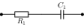
\includegraphics[width=3.125in,height=\textheight,keepaspectratio]{lec/../images/lec/lec5s2.png}

}

\caption{\label{fig-lec5s2}RC-Schaltung für eine Ortskurve}

\end{figure}%

\[
\underline{Z} = R_1 + \frac{1}{j \omega C_1} 
\]

\begin{Shaded}
\begin{Highlighting}[]
\ImportTok{import}\NormalTok{ numpy }\ImportTok{as}\NormalTok{ np}
\ImportTok{import}\NormalTok{ matplotlib.pyplot }\ImportTok{as}\NormalTok{ plt}

\CommentTok{\# Spezifikation der Impedanz/Admittanz}
\NormalTok{R }\OperatorTok{=} \FloatTok{2e3}
\NormalTok{C }\OperatorTok{=} \FloatTok{156e{-}9}

\NormalTok{f }\OperatorTok{=}\NormalTok{ np.linspace(}\FloatTok{0.2e3}\NormalTok{, }\FloatTok{5e3}\NormalTok{, }\DecValTok{5}\NormalTok{)}
\NormalTok{w }\OperatorTok{=} \DecValTok{2}\OperatorTok{*}\NormalTok{np.pi}\OperatorTok{*}\NormalTok{f}

\NormalTok{Z }\OperatorTok{=}\NormalTok{ R }\OperatorTok{+} \DecValTok{1}\OperatorTok{/}\NormalTok{(}\OtherTok{1j}\OperatorTok{*}\NormalTok{w}\OperatorTok{*}\NormalTok{C)}

\CommentTok{\# Ortskurve der Impedanz}
\NormalTok{plt.plot(Z.real, Z.imag, }\StringTok{\textquotesingle{}{-}x\textquotesingle{}}\NormalTok{)}
\NormalTok{plt.grid()}
\NormalTok{plt.xlabel(}\VerbatimStringTok{r\textquotesingle{}Re\{Z\}\textquotesingle{}}\NormalTok{)}
\NormalTok{plt.ylabel(}\VerbatimStringTok{r\textquotesingle{}Im\{Z\}\textquotesingle{}}\NormalTok{)}

\NormalTok{plt.show()}
\end{Highlighting}
\end{Shaded}

\pandocbounded{
\includegraphics[keepaspectratio]{lec/lec_05_files/figure-pdf/cell-3-output-1.png}}

``Die Ortskurve kann auch für die Parallelschaltung von R und C mit der
Frequenz als Parameter gezeichnet werden. Im Polardiagramm wird sie
durch die Zeiger aller Gesamtleitwerte oder Admittanzen gebildet und
verläuft im 1. Quadranten parallel zur imaginären Achse. Die
Achsenbezeichnungen der Leitwerte werden in Siemens (S) angeben. Die
Phasenwinkel sind auf die reelle (Re) Achse bezogen positiv.'' (Mietke
2024)

\subsection{Inversion von Ortskurven}\label{inversion-von-ortskurven}

``Bei der Konstruktion einer Ortskurve ist es oft notwendig von der
Widerstandsform \(\underline{Z}(\omega)\) auf die Leitwertsform
\(\underline{Y}(\omega)\) überzugehen und umgekehrt. Beide Funktionen
gehen jeweils aus der Kehrwertbildung der anderen hervor, man nennt sie
zueinander inverse Funktionen und die Kehrwertbildung selbst
Inversion.'' Kap. 5, (Büttner 2014)

Die Inversion der Ortskurve hat als Ergebnis die zur Ausgangsschaltung
äquivalente Schaltung. Diese Umrechnung ist immer dann notwendig, wenn
es sich um gemischte Reihen- und Parallelschaltungen wie bei T- und
\(\Pi\)-Filtern, belasteten Filtern und Schwingkreisen handelt.

Die Ortskurven einfacher RC- und RL-Schaltungen verhalten sich wie
folgt:

\begin{itemize}
\item
  Verläuft die Ortskurve der Impedanz oder Admittanz im 1. Quadranten,
  so befindet sich die dazu invertierte Ortskurve im 4. Quadranten.
\item
  Die Ortskurve der Impedanz einer Reihenschaltung ist eine Parallele
  zur imaginären Achse im Abstand des ohmschen Widerstandswerts. Die
  invertierte Ortskurve der Admittanz ist ein im Nullpunkt endender
  Halbkreis mit dem Durchmesser des reellen Leitwerts.
\item
  Die Ortskurve der Admittanz einer Parallelschaltung ist eine Parallele
  zur imaginären Achse im Abstand des reellen Leitwerts. Die invertierte
  Ortskurve der Impedanz ist ein im Nullpunkt endender Halbkreis mit dem
  Durchmesser des ohmschen Widerstandswerts.
\item
  Inversion eines Punktes (Widerstandsform/Impedanz):
  \(\underline{Z} (5 + 5j) \Omega\)
\item
  Ma\{\ss\}stäbe \(M_Z = 2 \Omega/cm\) und \(M_Y = 0.1 S/cm\)
\item
  Leitwertform/Admittanz: \(\underline{Y} = 1 / \underline{Z}\)
\end{itemize}

\[
\underline{Y} = \frac{1}{(5 + 5j) \Omega} = \frac{(5 - 5j)S}{50} = (0.1 - 0.1j) S
\]

\begin{itemize}
\tightlist
\item
  Inversion von Ortskuven durch Inversion einzelner Punkte:
\end{itemize}

\begin{enumerate}
\def\labelenumi{\arabic{enumi}.}
\item
  In die komplexe Zahlenebene wird der Zeiger \(Z\) eingetragen, dessen
  Spitze invertiert werden soll.
\item
  Um den Ursprung des Koordinatensystems wird ein Inversionskreis mit
  beliebigem Radius \(r\) geschlagen.
\item
  Von der Spitze des Zeigers \(Z\) aus werden Tangenten an den Kreis
  gelegt, sie ergeben die Berührungspunkte \(T_1\) und \(T_2\). Die
  Tangentenpunkte kann man auch finden, wenn man um die Mitte des
  Zeigers einen Kreis mit dem Radius \(Z / 2\), d.h. einen Thaleskreis,
  schlägt (siehe
  \href{https://de.wikipedia.org/wiki/Höhensatz}{Höhensatz}).
\item
  Die beiden Punkte \(T_1\) und \(T_2\) werden miteinander verbunden.
\item
  Wo die Verbindungslinie den Zeiger \(Z\) schneidet, liegt die Spitze
  des konjugiert komplexen Zeigers \(Y^*\).
\item
  Spiegelt man den Zeiger \(Y^*\) an der reellen Achse, so erhält man
  \(Y\). Die Spitze dieses Zeigers entspricht also der invertierten
  Spitze von \(Z\).
\item
  Bezeichnet man die Maßstäbe für den komplexen Scheinwiderstand mit
  \(M_Z\) und den Scheinleitwert mit \(M_Y\) sowie die Länge des Zeigers
  \(Z\) mit \(L_Z\) und die der Zeiger \(Y\) bzw. \(Y^*\) mit \(L_Y^*\)
  bzw. \(L_Y\), so ist -- da das Dreieck 0T1P rechtwinklig ist -- nach
  dem
  \href{https://de.wikipedia.org/wiki/Satzgruppe_des_Pythagoras\#Kathetensatz_des_Euklid}{Kathetensatz}
\end{enumerate}

\section{RC-Filter}\label{rc-filter}

\subsection{RC-Tiefpaß}\label{rc-tiefpauxdf}

\subsection{RC-Hochpaß}\label{rc-hochpauxdf}

\subsection{RC-Bandpaß}\label{rc-bandpauxdf}

\begin{figure}

\centering{

\includegraphics[width=4.16667in,height=\textheight,keepaspectratio]{lec/../images/lec/lec5bp.pdf}

}

\caption{\label{fig-lec5bp}Bode-Diagramm eines Bandpasses}

\end{figure}%

``Besitzt ein Netzwerk sowohl bei hohen als auch bei tiefen Frequenzen
einen Sperrbereich und bei mittleren Frequenzen einen Durchlaßbereich,
so liegt ein Bandpaß vor. Der prinzipielle Verlauf der
Spannungsverstärkung \(a_v\) ist im Bode-Diagramm
\{numref\}\texttt{fig:lec5bp} skizziert. Die Grenzen des
Durchlaßbereichs werden nach unten durch die untere Grenzfrequenz
\(f_{gu}\) und nach oben durch die obere Grenzfrequenz \(f_{go}\)
bestimmt. Die Differenz \(B = f_{go} − f_{gu}\) heißt Bandbreite (engl.
bandwidth) des Bandpasses; das geometrische Mittel

\[
f_m = \sqrt{f_{gu} f_{go}}
\]

der beiden Grenzfrequenzen wird als Bandmittenfrequenz bezeichnet. Bei
logarithmisch unterteilter Frequenzskala liegt \(f_m\) genau in der
Mitte zwischen \(f_{gu}\) und \(f_{go}\). Ein Bandpaß heißt
schmalbandig, falls \(B << f_m\) gilt; als Maß gilt die relative
Bandbreite \(B/f_m\). Die Abschwächung des Signals bei der
Bandmittenfrequenz wird als Einfügungsdämpfung bezeichnet.'' (Reisch
2007)

``Die als
\href{https://www.elektroniktutor.de/analogtechnik/wien.html}{Wien-Glied}
bezeichnete Schaltung ist ein spezieller RC-Bandpass. Im
Wien-Robinson-Generator bestimmt dieses Filter die Ausgangsfrequenz. Er
generiert Sinusfrequenzen mit sehr geringem Klirrfaktor. Im
durchstimmbaren Sinusgenerator sind die beiden Widerstände durch
gemeinsam einstellbare Potentiometer ersetzt. Diese Anordnung gibt es
auch in Wechselstrom-Brückenschaltungen.'' \{cite\}\texttt{mietke2024}

\section{Elementtransformation}\label{elementtransformation}

\begin{figure}

\centering{

\pandocbounded{\includegraphics[keepaspectratio]{lec/../images/lec/lec5ElemTransf.pdf}}

}

\caption{\label{fig-lec5ElemTransf}Tabelle der Elementtransformationen
TP zu HP, zu BP und zu BS}

\end{figure}%

Entn. aus (Deliyannis, Sun, und Fidler 1998)

\section{Messbrücken}\label{messbruxfccken}

\subsection{Wheatstone-Messbrücke --
Gleichstrommessbrücke}\label{wheatstone-messbruxfccke-gleichstrommessbruxfccke}

Zwei mögliche Messverfahren:

\begin{enumerate}
\def\labelenumi{\arabic{enumi}.}
\item
  Ausschlagverfahren Brückenspannung \(U_D\) wird mit hochohmigem
  Messinstrument gemessen.
\item
  Abgleich- oder Nullverfahren Brückenspannung \(U_D\) wird zu Null
  abgeglichen.
\end{enumerate}

\subsection{Wechselstrommessbrücke}\label{wechselstrommessbruxfccke}

\begin{itemize}
\tightlist
\item
  Abgleichbedingung
\end{itemize}

\[
\underline{Z}_1 \underline{Z}_4 = \underline{Z}_2 \underline{Z}_3
\]

\begin{itemize}
\tightlist
\item
  Zerlegung in Betrag und Phase
\end{itemize}

\begin{align}
\vert\underline{Z}_1\vert \vert\underline{Z}_4\vert &= \vert\underline{Z}_2\vert \vert\underline{Z}_3\vert \\
\varphi_1 + \varphi_4 &= \varphi_2 + \varphi_3
\end{align}

\begin{itemize}
\tightlist
\item
  Zerlegung in Real- und Imaginärteil
\end{itemize}

\begin{align}
R_1 R_4 - X_1 X_4 &= R_2 R_3 - X_2 X_3 \\
X_1 R_4 + R_1 X_4 &= X_2 R_3 + R_2 X_3
\end{align}

\begin{itemize}
\tightlist
\item
  zwei Bedingungen \(\Rightarrow\) zwei abgleichbare Elemente
\end{itemize}

\subsection{Kapazitätsmessbrücke nach Wien --
Wien-Brücke}\label{kapazituxe4tsmessbruxfccke-nach-wien-wien-bruxfccke}

\subsection{Wien-Robinson-Brücke -- einfaches
Frequenzmessgerät}\label{wien-robinson-bruxfccke-einfaches-frequenzmessgeruxe4t}

(Wikipedia 2019) (Hewlett 1942)

\chapter{Schwingkreise}\label{schwingkreise}

\begin{tcolorbox}[enhanced jigsaw, arc=.35mm, opacityback=0, opacitybacktitle=0.6, left=2mm, breakable, title=\textcolor{quarto-callout-note-color}{\faInfo}\hspace{0.5em}{Schwingungen (phys.)}, bottomrule=.15mm, toptitle=1mm, rightrule=.15mm, titlerule=0mm, leftrule=.75mm, colframe=quarto-callout-note-color-frame, colbacktitle=quarto-callout-note-color!10!white, bottomtitle=1mm, colback=white, toprule=.15mm, coltitle=black]

``Schwingungen begleiten uns im Alltag wörtlich auf Schritt und Tritt:
In jeder Uhr findet eine Schwingung statt, die zur Zeitmessung verwendet
wird. Das fängt bei dem Pendel der altmodischen Pendeluhr an und endet
nicht bei der modernen Quarzuhr, in der ein kleines Quarzplättchen
mechanische Schwingungen vollführt. Der Prozessor Ihres Smartphones
erhält seinen elektrischen Takt ebenfalls von einem solchen
Schwingquarz. Wenn wir sprechen, schwingen die Stimmlippen in unserem
Kehlkopf und verursachen so den primären Schall, der unsere Stimme
formt. Mechanische Konstruktionen und Bauwerke können ebenfalls in
Schwingungen geraten, wenn eine äußere Kraft auf sie einwirkt, was in
vielen Fällen unerwünscht ist. Auch in elektronischen Systemen finden
Schwingungen statt. Hier ändert sich nicht eine mechanische Auslenkung
als Funktion der Zeit, sondern eine elektrische Spannung oder ein
elektrischer Strom.

Sehr viele Phänomene, die bei schwingenden Systemen auftreten, kann man
exemplarisch an einfachen mechanischen Systemen studieren. In den
einführenden Physikbüchern wird sich dabei meist auf lineare Systeme
beschränkt, die zu harmonischen Schwingungen führen. Eine Schwingung
bezeichnet man als harmonisch, wenn sie sich durch eine reine Sinus-
oder Kosinusfunktion beschreiben lässt. Die Auslenkung \(x(t)\) bei
einer harmonischen Schwingung lässt sich durch

\[
x(t) = \hat{x} \cos(\omega t + \varphi)
\]

beschreiben. Dabei bezeichnet \(\hat{x}\) die Amplitude der Schwingung,
\(\varphi\) ist der Phasenwinkel und \(\omega\) die Kreisfrequenz der
Schwingung, die mit der Frequenz \(f\) über den Faktor \(2 \pi\)
verknüpft ist.

Für die Beschränkung auf harmonische Schwingungen gibt es zwei Gründe:
Zum einen lassen sich solche linearen Systeme gut analytisch behandeln,
und zum anderen lassen sich viele nichtlineare Systeme für hinreichend
kleine Auslenkungen gut durch entsprechende lineare Systeme annähern.
Für die Behandlung von schwingungsfähigen Systemen mit dem Computer
bieten sich zwei Aspekte besonders an: Wir können die Effekte der
linearen Schwingungsphysik visualisieren und zum Teil auch hörbar
machen, um damit ein intuitiveres Verständnis dieser Phänomene zu
gewinnen. Darüber hinaus bieten uns die in diesem Buch bereits
besprochenen Verfahren die Möglichkeit, auch nichtlineare Schwingungen
zu untersuchen.'' Entn. (Natt 2020)

\end{tcolorbox}

\begin{tcolorbox}[enhanced jigsaw, arc=.35mm, opacityback=0, opacitybacktitle=0.6, left=2mm, breakable, title=\textcolor{quarto-callout-note-color}{\faInfo}\hspace{0.5em}{Schwingkreise (elek.)}, bottomrule=.15mm, toptitle=1mm, rightrule=.15mm, titlerule=0mm, leftrule=.75mm, colframe=quarto-callout-note-color-frame, colbacktitle=quarto-callout-note-color!10!white, bottomtitle=1mm, colback=white, toprule=.15mm, coltitle=black]

``Eine physikalische Anordnung ist schwingungsfähig, wenn sie mindestens
zwei Energiespeicher unterschiedlichen physikalischen Charakters
enthält, die miteinander Energie austauschen kön- nen. Eine solche
Anordnung wird als Schwingkreis bezeichnet.

In elektrischen Schaltungen sind diese unterschiedlichen Typen von
Energiespeichern Induktivitäten, die magnetische Feldenergie speichern
und Kapazitäten zur Speicherung elektrischer Feldenergie.

Die in einer Kapazität gespeicherte Energie wird durch den Wert C der
Kapazität und die Spannung u an der Kapazität bestimmt, die in einer
Induktivität gespeicherte Energie durch den Wert L der Induktivität und
den Strom i durch die Induktivität.

Zu unterscheiden ist zwischen freien und erzwungenen Schwingungen. Bei
freien Schwingungen {[}\ldots{]} wird einer physikalischen Anordnung
einmalig Energie zugeführt und sie sich dann selbst überlassen. Durch
unvermeidliche Verlustmechanismen, die dazu führen, dass im Schwingkreis
pendelnde Energie in Wärme umgesetzt wird, klingt die Schwingung
zeitlich ab. Bei erzwungenen Schwingungen {[}\ldots{]} wird einer
zunächst energielosen Anordnung periodisch von außen Energie zugeführt.
Ein Teil dieser Energie wird zur Kompensation der mit der
Schwingungsintensität ansteigenden Verluste benötigt, der Rest pendelt
zwischen den Energiespeichern. Ändert sich die Art der periodischen
Energiezufuhr nicht, so stellt sich nach einem Einschwingvorgang in der
Anordnung eine stationäre Schwingung (eingeschwungener Zustand) ein.''
Entn. (Harriehausen und Schwarzenau 2020)

\end{tcolorbox}

\section{Zusammenfassung der physikalische
Grundlagen}\label{zusammenfassung-der-physikalische-grundlagen}

\begin{itemize}
\item
  periodische Zustandsänderung in einem physikalischen System
\item
  periodischer Energieaustausch zw. zwei unterschiedlichen
  Energiespeichern (potentiellen und kinetischen), z.B. Feder und Masse,
  Induktivität und Kapazität
\item
  maßgebende Zustandsgröße \(x(t)\), z.B. Auslenkung, Spannung oder
  Ladung, folgen einer gewöhnlichen Differenzialgleichung (DGL)
  \(\ddot{x} + \omega_0 x = 0\)
\item
  harmonische Schwingung, \(x(t+T_0) = x(t)\), wobei \(T_0\) Periode,
  \(\omega_0=2 \pi f_0 = 2\pi \frac{1}{T_0}\) Eigenfrequenz und \(f_0\)
  Resonanzfrequenz
\item
  DGL gehorcht dem Energieerhaltungssatz
\end{itemize}

\begin{align}
W_{ges}(x) &= W_{pot}(x) + W_{kin}(x) = const. \\
\frac{d W_{ges}}{dt} &= \frac{dW_{pot}}{dx} \frac{dx}{dt} + \frac{d W_{kin}}{dx} \frac{d x}{dt} = 0 \\
x(t) &= x_{max} \cos(\omega_0 t + \varphi_0)
\end{align}

\begin{itemize}
\tightlist
\item
  Zusammenschaltung von Induktivität \(L\) und Kapazität \(C\) heißt
  (idealer) Schwing- oder Resonanzkreis
\end{itemize}

\begin{align}
W_{pot} &:= \mbox{Kondensator} \\
W_{kin} &:= \mbox{Induktivität}
\end{align}

\begin{itemize}
\item
  freie und erzwungene Schwingung
\item
  ungedämpfte und gedämpfte Schwingung
\end{itemize}

\section{RLC-Reihenschwingkreis (aktiver
Zweipol)}\label{rlc-reihenschwingkreis-aktiver-zweipol}

\begin{figure}

\centering{

\includegraphics[width=4.16667in,height=\textheight,keepaspectratio]{lec/../images/lec/lec6rlc.pdf}

}

\caption{\label{fig-lec6rlc}RLC-Reihenschwingkreis}

\end{figure}%

\begin{tcolorbox}[enhanced jigsaw, arc=.35mm, opacityback=0, opacitybacktitle=0.6, left=2mm, breakable, title=\textcolor{quarto-callout-note-color}{\faInfo}\hspace{0.5em}{Maschengleichung (Zeitbereich)}, bottomrule=.15mm, toptitle=1mm, rightrule=.15mm, titlerule=0mm, leftrule=.75mm, colframe=quarto-callout-note-color-frame, colbacktitle=quarto-callout-note-color!10!white, bottomtitle=1mm, colback=white, toprule=.15mm, coltitle=black]

\begin{align}
u_1(0) &= L \frac{di}{dt} + i\, R + \frac{1}{C} \int i dt  \\
0 &= \frac{di}{dt^2} + \frac{R}{L} \frac{di}{dt} + \frac{1}{LC} i
\end{align}

\end{tcolorbox}

\begin{tcolorbox}[enhanced jigsaw, arc=.35mm, opacityback=0, opacitybacktitle=0.6, left=2mm, breakable, title=\textcolor{quarto-callout-note-color}{\faInfo}\hspace{0.5em}{Lösung der Differentialgleichung}, bottomrule=.15mm, toptitle=1mm, rightrule=.15mm, titlerule=0mm, leftrule=.75mm, colframe=quarto-callout-note-color-frame, colbacktitle=quarto-callout-note-color!10!white, bottomtitle=1mm, colback=white, toprule=.15mm, coltitle=black]

\[
i(t) = \underbrace{I_0 e^{-d \omega_0 t}}_{Dämpfung} \underbrace{\sin\left(\sqrt{1 -d^2} \omega_0 t\right)}_{harm. Schwingung}
\]

\end{tcolorbox}

\begin{tcolorbox}[enhanced jigsaw, arc=.35mm, opacityback=0, opacitybacktitle=0.6, left=2mm, breakable, title=\textcolor{quarto-callout-note-color}{\faInfo}\hspace{0.5em}{Spannungsübertragungsfaktor}, bottomrule=.15mm, toptitle=1mm, rightrule=.15mm, titlerule=0mm, leftrule=.75mm, colframe=quarto-callout-note-color-frame, colbacktitle=quarto-callout-note-color!10!white, bottomtitle=1mm, colback=white, toprule=.15mm, coltitle=black]

Entn. (Reisch 2007)

\begin{align}
\underline{H}_u(j \omega) = \frac{\underline{U}_2}{\underline{U}_1} &= \frac{1}{1 + j \omega R C + \omega^2 LC} \\
&= \frac{1}{1 + j \frac{\omega}{\omega_0 Q} + \left(\frac{\omega}{\omega_0}\right)^2}
\end{align}

\begin{itemize}
\item
  Eigenfrequenz / Resonanzfrequenz \(\omega_0 = \frac{1}{\sqrt{L C}}\)
\item
  Abklingkonstante \(\delta = \frac{R}{\omega_0 L}\)
\item
  Dämpfung / Verlustfaktor
  \(d = \frac{1}{Q} = \frac{R}{\omega_0 L} = \frac{2 \delta}{\omega_0}\)
\item
  Güte
  \(Q = \frac{\vert Q(\omega_0) \vert}{P(\omega_0)} = \frac{1}{\omega_0 RC} = \frac{\omega_0}{2 \delta}\)

  \begin{itemize}
  \tightlist
  \item
    \(\vert Q(\omega_0) \vert\) ist der Betrag der Blindleistung
  \item
    \(P(\omega_0)\) ist die Wirkleistung
  \end{itemize}
\item
  Analyse mit LTspice und Python
  \href{https://github.com/DongHoonPark/ltspice_pytool}{GitHub}
  Installation mit Anaconda-Shell oder Windows-Shell (CMD/PowerShell)
\end{itemize}

\begin{Shaded}
\begin{Highlighting}[]
\NormalTok{$ pip install {-}U ltspice}
\end{Highlighting}
\end{Shaded}

\end{tcolorbox}

\begin{Shaded}
\begin{Highlighting}[]
\ImportTok{import}\NormalTok{ ltspice}
\ImportTok{import}\NormalTok{ numpy }\ImportTok{as}\NormalTok{ np}
\ImportTok{import}\NormalTok{ matplotlib.pyplot }\ImportTok{as}\NormalTok{ plt}

\CommentTok{\# \%\% Laden der RAW LTspice Daten in den Python{-}Workspace}
\BuiltInTok{file} \OperatorTok{=} \StringTok{"../files/spice/kap137\_reisch.raw"}
\NormalTok{data }\OperatorTok{=}\NormalTok{ ltspice.Ltspice(}\BuiltInTok{file}\NormalTok{)}
\NormalTok{data.parse()}

\CommentTok{\# \%\% Zuweisen der Simulationdaten an lokale Variablen}
\NormalTok{Hu }\OperatorTok{=}\NormalTok{ data.get\_data(}\StringTok{"v(vo)"}\NormalTok{)}
\NormalTok{freq }\OperatorTok{=}\NormalTok{ data.get\_data(}\StringTok{"frequency"}\NormalTok{)}

\CommentTok{\# \%\% Daten werden als Numpy{-}Array geladen, Typ complex}
\NormalTok{Hu\_dB }\OperatorTok{=} \DecValTok{20}\OperatorTok{*}\NormalTok{np.log10(np.}\BuiltInTok{abs}\NormalTok{(Hu))}
\NormalTok{Hu\_arg }\OperatorTok{=} \DecValTok{180} \OperatorTok{/}\NormalTok{ np.pi }\OperatorTok{*}\NormalTok{ np.angle(Hu)}
\NormalTok{f }\OperatorTok{=}\NormalTok{ freq.real}

\CommentTok{\# \%\% Erzeugen des Bode{-}Diagramms (Plot)}
\NormalTok{fig1 }\OperatorTok{=}\NormalTok{ plt.figure(}\DecValTok{1}\NormalTok{)}
\NormalTok{plt.subplot(}\DecValTok{2}\NormalTok{, }\DecValTok{1}\NormalTok{, }\DecValTok{1}\NormalTok{)}
\NormalTok{plt.semilogx(f, Hu\_dB)}
\NormalTok{plt.grid()}
\NormalTok{plt.ylabel(}\VerbatimStringTok{r\textquotesingle{}}\DecValTok{$}\VerbatimStringTok{H\_u}\KeywordTok{(}\VerbatimStringTok{f}\KeywordTok{)}\DecValTok{$}\VerbatimStringTok{/dB\textquotesingle{}}\NormalTok{)}
\NormalTok{plt.subplot(}\DecValTok{2}\NormalTok{, }\DecValTok{1}\NormalTok{, }\DecValTok{2}\NormalTok{)}
\NormalTok{plt.grid()}
\NormalTok{plt.semilogx(f, Hu\_arg)}
\NormalTok{plt.ylabel(}\VerbatimStringTok{r\textquotesingle{}arg}\KeywordTok{(}\DecValTok{$}\VerbatimStringTok{H\_u}\KeywordTok{(}\VerbatimStringTok{f}\KeywordTok{)}\DecValTok{$}\KeywordTok{)}\VerbatimStringTok{/deg\textquotesingle{}}\NormalTok{)}
\NormalTok{plt.xlabel(}\StringTok{\textquotesingle{}Frequenz f/Hz\textquotesingle{}}\NormalTok{)}
\NormalTok{plt.show()}
\end{Highlighting}
\end{Shaded}

\section{Grundeigenschaften von Reihen- und Parallelschwingkreis
(passiver
Zweipol)}\label{grundeigenschaften-von-reihen--und-parallelschwingkreis-passiver-zweipol}

\begin{tcolorbox}[enhanced jigsaw, arc=.35mm, opacityback=0, opacitybacktitle=0.6, left=2mm, breakable, title=\textcolor{quarto-callout-note-color}{\faInfo}\hspace{0.5em}{Resonanzfrequenz}, bottomrule=.15mm, toptitle=1mm, rightrule=.15mm, titlerule=0mm, leftrule=.75mm, colframe=quarto-callout-note-color-frame, colbacktitle=quarto-callout-note-color!10!white, bottomtitle=1mm, colback=white, toprule=.15mm, coltitle=black]

\begin{itemize}
\item
  Thomsonsche Formel
  \(\omega_0 = \frac{1}{L_r C_r} = \frac{1}{L_p C_p}\)
\item
  bei Resonanz erreichen Impedanz und Admittanz ein Minimum
\end{itemize}

\begin{align}
\left . \underline{Z} \right\lvert_{\omega_0} &\Rightarrow \lvert\underline{Z}\lvert = R_r \\
\left . \underline{Y} \right\lvert_{\omega_0} &\Rightarrow \lvert\underline{Y}\lvert = G_p
\end{align}

\begin{longtable}[]{@{}lll@{}}
\toprule\noalign{}
& \(X(\omega)\) & \(B(\omega)\) \\
\midrule\noalign{}
\endhead
\bottomrule\noalign{}
\endlastfoot
\(\omega < \omega_0\) & \emph{kapazitiv} & \emph{induktiv} \\
\(\omega > \omega_0\) & \emph{induktiv} & \emph{kapazitiv} \\
\end{longtable}

\end{tcolorbox}

\begin{tcolorbox}[enhanced jigsaw, arc=.35mm, opacityback=0, opacitybacktitle=0.6, left=2mm, breakable, title=\textcolor{quarto-callout-note-color}{\faInfo}\hspace{0.5em}{Reihenkreis (Impedanz)}, bottomrule=.15mm, toptitle=1mm, rightrule=.15mm, titlerule=0mm, leftrule=.75mm, colframe=quarto-callout-note-color-frame, colbacktitle=quarto-callout-note-color!10!white, bottomtitle=1mm, colback=white, toprule=.15mm, coltitle=black]

\begin{align}
\underline{Z} &= R_r + j\left(\omega L_r - \frac{1}{\omega C_r}\right) \\
&= R_r + j X(\omega) \\
\lvert\underline{Z}\lvert &= \sqrt{R_r^2 + X^2(\omega)} \\
\arg{\underline{Z}} &= \arctan \frac{X(\omega)}{R_r}
Q = \frac{\omega_0 L}{R} = \frac{1}{R}\sqrt{\frac{L}{C}}
\end{align}

\end{tcolorbox}

\begin{tcolorbox}[enhanced jigsaw, arc=.35mm, opacityback=0, opacitybacktitle=0.6, left=2mm, breakable, title=\textcolor{quarto-callout-note-color}{\faInfo}\hspace{0.5em}{Parallelkreis (Admittanz)}, bottomrule=.15mm, toptitle=1mm, rightrule=.15mm, titlerule=0mm, leftrule=.75mm, colframe=quarto-callout-note-color-frame, colbacktitle=quarto-callout-note-color!10!white, bottomtitle=1mm, colback=white, toprule=.15mm, coltitle=black]

\begin{align}
\underline{Y} &= G_p + j\left(\omega C_p- \frac{1}{\omega L_p}\right) \\
&= G_r + j B(\omega) \\
\lvert\underline{Y}\lvert &= \sqrt{G_p^2 + B^2(\omega)} \\
\arg{\underline{Y}} &= \arctan \frac{B(\omega)}{G_p}
Q &= \frac{\omega_0 C}{G} = \frac{1}{G}\sqrt{\frac{C}{L}}
\end{align}

\end{tcolorbox}

\section{Vereinheitlichte
Kennzeichnung}\label{vereinheitlichte-kennzeichnung}

\begin{tcolorbox}[enhanced jigsaw, arc=.35mm, opacityback=0, opacitybacktitle=0.6, left=2mm, breakable, title=\textcolor{quarto-callout-note-color}{\faInfo}\hspace{0.5em}{Verstimmung \(v\), relative Frequenzabweichung}, bottomrule=.15mm, toptitle=1mm, rightrule=.15mm, titlerule=0mm, leftrule=.75mm, colframe=quarto-callout-note-color-frame, colbacktitle=quarto-callout-note-color!10!white, bottomtitle=1mm, colback=white, toprule=.15mm, coltitle=black]

\begin{align}
v &= \frac{\omega}{\omega_0}-\frac{\omega_0}{\omega}
\end{align}

\end{tcolorbox}

\begin{tcolorbox}[enhanced jigsaw, arc=.35mm, opacityback=0, opacitybacktitle=0.6, left=2mm, breakable, title=\textcolor{quarto-callout-note-color}{\faInfo}\hspace{0.5em}{Normierte Darstellung}, bottomrule=.15mm, toptitle=1mm, rightrule=.15mm, titlerule=0mm, leftrule=.75mm, colframe=quarto-callout-note-color-frame, colbacktitle=quarto-callout-note-color!10!white, bottomtitle=1mm, colback=white, toprule=.15mm, coltitle=black]

\begin{align}
\underline{Z} &= R \left( 1 + j \frac{1}{R} \left( \frac{\omega \omega_0 \omega L}{\omega_0}
- \frac{\omega_0}{\omega_0 \omega C}\right)\right) \\
&= R (1 + Q v) \\
\underline{Y} &= G (1 + j Q v)
\end{align}

\end{tcolorbox}

\begin{tcolorbox}[enhanced jigsaw, arc=.35mm, opacityback=0, opacitybacktitle=0.6, left=2mm, breakable, title=\textcolor{quarto-callout-note-color}{\faInfo}\hspace{0.5em}{Betrag und Phase}, bottomrule=.15mm, toptitle=1mm, rightrule=.15mm, titlerule=0mm, leftrule=.75mm, colframe=quarto-callout-note-color-frame, colbacktitle=quarto-callout-note-color!10!white, bottomtitle=1mm, colback=white, toprule=.15mm, coltitle=black]

\begin{align}
\frac{\lvert\underline{Z}\lvert}{R} = \frac{\lvert \underline{Y}\lvert}{G} &= \sqrt{1 + \left( Q v \right)} \\
\varphi_Z = \varphi_Y &= \arctan\left( Q v \right)
\end{align}

\end{tcolorbox}

\begin{tcolorbox}[enhanced jigsaw, arc=.35mm, opacityback=0, opacitybacktitle=0.6, left=2mm, breakable, title=\textcolor{quarto-callout-note-color}{\faInfo}\hspace{0.5em}{45\(^{\circ}\)-, \(\frac{\pi}{4}\)- oder 3dB-Frequenz}, bottomrule=.15mm, toptitle=1mm, rightrule=.15mm, titlerule=0mm, leftrule=.75mm, colframe=quarto-callout-note-color-frame, colbacktitle=quarto-callout-note-color!10!white, bottomtitle=1mm, colback=white, toprule=.15mm, coltitle=black]

Der Phasenwinkel \(\varphi\) ist gleich 45\(^{\circ}\) und Betrag der
Blindkomponente ist gleich der Wirkkomponente.

\begin{align}
\lvert X(\omega_{\pm 45}) \lvert &= \pm R &  \lvert B(\omega_{\pm 45}) \lvert &= \pm G \\
\omega_{\pm 45} L - \frac{1}{\omega_{\pm 45} C} &= \pm R &  \omega_{\pm 45} C - \frac{1}{\omega_{\pm 45} L} &= \pm G
\end{align}

\begin{align}
\omega_{\pm 45} &= \omega_0 \left( \sqrt{1 + \left(\frac{1}{2Q}\right)^2} \pm \frac{1}{2Q}\right) \approx \omega_0 \left( 1 \pm \frac{1}{2Q}\right)
\end{align}

\begin{align}
\lvert \underline{Z(\omega_{\pm 45})} \lvert &= \sqrt{2} R &  \lvert \underline{Y(\omega_{\pm 45})} \lvert &= \sqrt{2} G
\end{align} \$\$

\end{tcolorbox}

\begin{tcolorbox}[enhanced jigsaw, arc=.35mm, opacityback=0, opacitybacktitle=0.6, left=2mm, breakable, title=\textcolor{quarto-callout-note-color}{\faInfo}\hspace{0.5em}{Bandbreite BW (bandwidth)}, bottomrule=.15mm, toptitle=1mm, rightrule=.15mm, titlerule=0mm, leftrule=.75mm, colframe=quarto-callout-note-color-frame, colbacktitle=quarto-callout-note-color!10!white, bottomtitle=1mm, colback=white, toprule=.15mm, coltitle=black]

\begin{align}
BW &= \omega_{45} - \omega_{-45} = \frac{\omega_0}{Q} \\
&= f_{45} - f_{-45} = \frac{f_0}{Q} \\
\end{align}

\end{tcolorbox}

\section{Gegenüberstellung der Eigenschaften der elementaren
Schwingkreise}\label{gegenuxfcberstellung-der-eigenschaften-der-elementaren-schwingkreise}

\begin{figure}

\centering{

\pandocbounded{\includegraphics[keepaspectratio]{lec/../images/lec/lec6elemSchwing.pdf}}

}

\caption{\label{fig-lec6elemSchwing}Eingenschaften von Schwingkreisen}

\end{figure}%

Entn. aus (Harriehausen und Schwarzenau 2020)

\chapter{Netzwerkanalyse}\label{netzwerkanalyse}

Entn. aus (Kasper 2000) (Paul und Paul 2019)

\section{Systemsimulation}\label{systemsimulation}

\begin{longtable}[]{@{}lrl@{}}
\toprule\noalign{}
Ebene & Maß & Simulation \\
\midrule\noalign{}
\endhead
\bottomrule\noalign{}
\endlastfoot
Atom & 0.1 nm & \\
Festkörper/Atomverbund & 1.0 nm & \\
Device & 0.1 mm & Feld \\
Transistor/Subkomponenten & 1.0 mm & \\
Gatter/Komponenten & 10 mm & Verhaltensmodell \\
\end{longtable}

\section{Makrotheorie}\label{makrotheorie}

\begin{itemize}
\item
  Mittelwerte charakteristischer Größen des Systems
\item
  Temperatur, Wärmekapazität, Leitfähigkeit etc.
\item
  schwache oder homogene Ortsabhängigkeit
\item
  partielle Differentialgleichungen (PDE's) der Feldtheorie gehen über
  in gewöhnliche Differentialgleichungen (ODE's)
\item
  nur noch dt kein dx (nach dem Ort)
\end{itemize}

\section{Netzwerksimulation}\label{netzwerksimulation}

\begin{itemize}
\item
  Maschenwiderstandsmatrix
\item
  Knotenleitwertmatrix
\item
  mathematisch äquivalente Beschreibungen
\item
  für praktische Berechnungen (Simulation) \(\rightarrow\) Knotenanalyse
\end{itemize}

\section{Netzwerk}\label{netzwerk}

\begin{figure}

\centering{

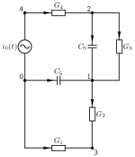
\includegraphics[width=4.16667in,height=\textheight,keepaspectratio]{lec/../images/lec/lec6s20.png}

}

\caption{\label{fig-lec7knoten}Netzwerk für die Knotenspannungsanalyse}

\end{figure}%

\subsection{Transiente Analyse}\label{transiente-analyse}

\begin{itemize}
\tightlist
\item
  Knoten 0:
\end{itemize}

\begin{align}
-i_0-i_1-i_5&=0 \\
-G_1(v_3-v_0) - C_5 \frac{d}{dt}(v_1-v_0) &= i_0
\end{align} \$\$

\begin{itemize}
\tightlist
\item
  Knoten 1:
\end{itemize}

\begin{align}
-i_2+i_3+i_5+i_6&=0 \\
-G_2(v_3-v_1)+G_3(v_1-v_3)+C_5 \frac{d}{dt}(v_1-v_0)+C_6 \frac{d}{dt}(v_1-v_6)&=0
\end{align}

\begin{itemize}
\tightlist
\item
  Knoten 2:
\end{itemize}

\begin{align}
-i_3+i_4-i_6 &= 0 \\
-G_3(v_1-v_2)+G_4(v_2-v_4)-C_6 \frac{d}{t}(v_1-v_2) &= 0
\end{align}

\subsection{Differentialgleichungssystem}\label{differentialgleichungssystem}

\begin{align}
\begin{pmatrix}
G_2+G_3 & -G_3 & -G_2 & 0 \\
-G_3 & G_3+G_4 & 0 & -G_4 \\
-G_2 & 0 & G_1+G_2 & 0 \\
0 & -G_4 & 0 & G_4
\end{pmatrix} & 
\begin{pmatrix}
v_1 \\
v_2 \\
v_3 \\
v_4
\end{pmatrix}
+ \cdots \\ 
\begin{pmatrix}
C_5+C_6 & -C_6 & 0 & 0 \\
-C_6 & C_6 & 0 & 0 \\
0 & 0 & 0 & 0 \\
0 & 0 & 0 & 0
\end{pmatrix}
\frac{d}{dt} &
\begin{pmatrix}
v_1 \\
v_2 \\
v_3 \\
v_4
\end{pmatrix}
=
\begin{pmatrix}
0 \\
0 \\
0 \\
-i_0
\end{pmatrix}
\end{align}

\begin{align}
\mathbf{A} \mathbf{x} + \mathbf{B} \dot{\mathbf{x}} &= \mathbf{b} \\
\dot{\mathbf{x}} &= -\mathbf{B}^{-1}\mathbf{A}\mathbf{x} +
\mathbf{B}^{-1}\mathbf{b}(t) \\
&= \mathbf{T}\mathbf{x} + \mathbf{g}(t)
\end{align}

\section{Netzwerkanalyse zeitabhängiger
Signale}\label{netzwerkanalyse-zeitabhuxe4ngiger-signale}

\begin{itemize}
\item
  Matrix \(\mathbf{B}\) ist nicht immer invertierbar, ggf. blockweise
  zerlegen
\item
  Algebro-Differentialgleichungen
\item
  Euler-Verfahren, explizit (vorwärts), implizit (rückwärts)
\item
  Trapez- oder Mittelpunktregel

  \begin{itemize}
  \item
    Adams-Bashforth-,Adams-Multon- und Gear-Verfahren
  \item
    \emph{Gut für den Rechner} \(\rightarrow\) Python, SPICE
  \item
    Wir machen Transformation und dann Gauss'sches-Eliminationsverfahren
  \end{itemize}
\end{itemize}

\section{Lösung im Frequenzbereich}\label{luxf6sung-im-frequenzbereich}

\begin{longtable}[]{@{}
  >{\raggedright\arraybackslash}p{(\linewidth - 4\tabcolsep) * \real{0.1340}}
  >{\raggedright\arraybackslash}p{(\linewidth - 4\tabcolsep) * \real{0.3196}}
  >{\raggedright\arraybackslash}p{(\linewidth - 4\tabcolsep) * \real{0.5464}}@{}}
\toprule\noalign{}
\begin{minipage}[b]{\linewidth}\raggedright
\end{minipage} & \begin{minipage}[b]{\linewidth}\raggedright
Zeitbereich
\end{minipage} & \begin{minipage}[b]{\linewidth}\raggedright
Frequenzbereich
\end{minipage} \\
\midrule\noalign{}
\endhead
\bottomrule\noalign{}
\endlastfoot
& Urbildbereich & Bildbereich \\
Spannung & \(u_n(t)\) &
\(\underline{u}(t)=\underline{\hat{U}}e^{j\omega t}\) \\
Strom & \(i_n(t)\) &
\(\underline{i}(t)=\underline{\hat{U}}e^{j\omega t}\) \\
Widerstand & \(u_R(t)=Ri_R(t)\) &
\(\underline{u}_R(t)=R \underline{i}(t)\) \\
Kondensator & \(i_C(t)=C \frac{du_C(t)}{dt}\) &
\(\underline{i}_C(t)= j \omega C \underline{u}_C(t)\) \\
Spule & \(u_L(t)=L \frac{di_L(t)}{dt}\) &
\(\underline{u}_L(t)= j \omega L \underline{i}_L(t)\) \\
& (wenn für \(t=0\) energielos) & \\
\end{longtable}

\section{Grundaufgabe der
Netzwerkanalyse}\label{grundaufgabe-der-netzwerkanalyse}

\begin{itemize}
\item
  Gewinnung des Netzwerkes
\item
  Wahl des Lösungsverfahrens
\item
  Durchführung der Netzwerkanalyse
\item
  Diskussion der Lösung
\end{itemize}

\section{Netzwerkgleichungen -- Kirchhoff'sche
Gesetze}\label{netzwerkgleichungen-kirchhoffsche-gesetze}

\begin{itemize}
\item
  Knotensatz: \(\sum i_n(t)=0\)
\item
  Maschensatz: \(\sum u_n(t)=0\)
\item
  Zweigbeziehungen: \(u_n = f(i_n)\)
\end{itemize}

\section{Vollständiges Kirchhoff'sches
Gleichungssystem}\label{vollstuxe4ndiges-kirchhoffsches-gleichungssystem}

\begin{itemize}
\item
  \(p=k-1\), unabhängige Knotengleichungen
\item
  \(m=z-(k-1)\), unabhängige Maschengleichungen
\item
  \(z\), \(u,i\)-Beziehungen der Zweigelemente
\end{itemize}

\section{Netzwerkstruktur}\label{netzwerkstruktur}

\subsection{Unabhängige Knoten und
Maschen}\label{unabhuxe4ngige-knoten-und-maschen}

Die Eigenschaften eines Netzwerkes werden von den Netzwerkelementen und
der Netzwerkstruktur oder -topologie bestimmt. Das ist die Art ihrer
Zusammenschaltung. Sie wird auch als ``Gerüst'' bezeichnet und
zeichnerisch durch den ``Streckenkomplex'' (engl. graph) ausgedrückt.
Die Beschreibung kann gleichwertig durch eine ``topologische Matrix''
erfolgen.

\subsection{Netzwerkgraph}\label{netzwerkgraph}

Der Netzwerkgraph beschreibt die Verbindung der Netzwerkelemente durch
Abstraktion der Netzwerkgeometrie. Jedem Knoten im Graphen entspricht
ein Knoten im Netzwerk und jeder Verbindungslinie ein Zweig zwischen
zwei Knoten. Er ist Grundlage der Zahl unabhängiger Knoten- und
Maschengleichungen und kann durch ``topologische Matrizen'' (sog.
``Inzidenzmatrizen'') mathematisch beschrieben werden.

\section{Vollständiger Baum}\label{vollstuxe4ndiger-baum}

Ein vollständiger Baum (engl. tree) ist ein Teilgraph, der keine Umläufe
besitzt und alle Knoten des Ausgangsgraphen miteinander verbindet. In
einem Netzwerk mit \(k\) Knoten hat der vollständige Baum insgesamt
\(k-1\) Zweige.

\subsection{Merkmale}\label{merkmale}

\begin{itemize}
\item
  alle Knoten sind direkt oder indirekt miteinander verbunden,
\item
  wird ein weiterer Zweig entfernt, so geht Merkmal 1. verloren,
\item
  es treten keine Umläufe auf.
\end{itemize}

\section{Baumkomplement}\label{baumkomplement}

Das Baumkomplement bildet als Gesamtheit aller Verbindungszweige das
``System unabhängiger Zweige''. Jeder Verbindungszweig gehört genau zu
einer Schleife (Masche), die nur aus diesem Verbindungszweig und Zweigen
des vollständigen Baumes besteht. Eine solche Schleife heißt
``Fundamentalschleife'' (``unabhängige Masche''). Davon gibt es
\(m=z-(k-1)\).

\section{Maschenstromverfahren}\label{maschenstromverfahren}

\begin{figure}

\centering{

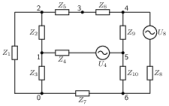
\includegraphics[width=4.16667in,height=\textheight,keepaspectratio]{lec/../images/lec/lec6s30.png}

}

\caption{\label{fig-lec7masch}Netzwerk für die Maschenstromanalyse}

\end{figure}%

\section{\texorpdfstring{Wahl der unabhängigen Ströme
\(I_M\)}{Wahl der unabhängigen Ströme I\_M}}\label{wahl-der-unabhuxe4ngigen-struxf6me-i_m}

\[
I_1, I_4, I_7, I_8 
\]

Abbildung der abhängigen Ströme durch die unabhängigen Ströme:

\begin{align}
\begin{pmatrix}
I_2 \\
I_3 \\
I_5 \\
I_6 \\
I_9 \\
I_{10}
\end{pmatrix}
=
\begin{pmatrix}
-1 & -1 & -1 & 0 \\
-1 & 0 & -1 & 0 \\
0 & -1 & -1 & 0 \\
0 & -1 & -1 & 0 \\
0 & 1 & 1 & -1 \\
0 & 0 & 1 & -1 \\
\end{pmatrix}
\begin{pmatrix}
I_1 \\
I_4 \\
I_7 \\
I_8
\end{pmatrix}
\end{align}

\section{4 Maschengleichungen}\label{maschengleichungen}

\begin{align}
I_1Z_1 - I_2Z_2 - I_3Z_3 &= 0 \\
U_4 + I_4Z_4 + I_9+Z_9 - I_6Z_6 - I_5Z_5 - I_2Z_2 &= 0 \\
I_7Z_7 + I_{10}Z_{10} + I_9Z_9 - I_6Z_6 - I_5Z_5 - I_2Z_2 -
I_3Z_3 &= 0 \\
U_8 + I_8Z_8 - I_9Z_9 - I_{10}Z_{10} &= 0
\end{align}

Sortieren und aufstellen des Gleichungssystems:

\begin{align}
\underbrace{\begin{pmatrix}
\sum Z_{1,3} & Z_2 & \sum Z_{2,3} & 0 \\
Z_2 & \sum Z_{2,4,5,6,9} & \sum Z_{2,5,6,9,10} & -Z_9 \\
\sum Z_{2,3} & \sum Z_{2,5,6,9,10} & \sum Z_{2,3,5,6,7,9,10} &
\sum -Z_{9,10} \\
0 & -Z_9 & \sum -Z_{9,10} & \sum Z_{8,9,10}
\end{pmatrix}}_{\mathbf{Z}}
\underbrace{\begin{pmatrix}
I_1 \\
I_4 \\
I_7 \\
I_8
\end{pmatrix}}_{\mathbf{I_M}}
&=
\underbrace{\begin{pmatrix}
0 \\
-U_4 \\
0 \\
-U_8
\end{pmatrix}}_{\mathbf{U}}
\end{align}

\section{Knotenspannungsanalyse}\label{knotenspannungsanalyse}

Beim Knotenspannungsverfahren, das auf Maxwell (1873) zurückgeht, wird
die Hilfsvariable \emph{Knotenspannung} so eingeführt, dass jede
\emph{Maschengleichung} automatisch erfüllt ist und daher alle
wegfallen.

Das Verfahren umfasst dann:

\begin{itemize}
\item
  die Aufstellung der Knotengleichungen für die Zweigströme,
\item
  ihren Ersatz durch die Zweigbeziehungen \(I=f(U)\) der
  Netzwerkelemente ausgedrückt durch Knotenspannungen
\end{itemize}

(statt der Zweigspannung) und die Lösung der Gleichungen nach den
Knotenspannungen.

\section{Knotenspannungs- vs
Maschenstromanalyse}\label{knotenspannungs--vs-maschenstromanalyse}

\begin{itemize}
\item
  Wegfall der Baumsuche, auch spielt die Zahl unabhängiger Maschen
  \(m = z-(k-1)\) und damit die Anzahl der Zweige keine Rolle,
\item
  weil die Knotenspannungen unabhängige Variablen sind, dürfen
  Spannungsquellen nicht auftreten, denn eine ideale Spannungsquelle
  zwischen zwei Knoten macht den Strom durch die Quelle unbestimmt.
\end{itemize}

\chapter{Spulen und Übertrager}\label{spulen-und-uxfcbertrager}

\begin{tcolorbox}[enhanced jigsaw, arc=.35mm, opacityback=0, opacitybacktitle=0.6, left=2mm, breakable, title=\textcolor{quarto-callout-note-color}{\faInfo}\hspace{0.5em}{Hinweis}, bottomrule=.15mm, toptitle=1mm, rightrule=.15mm, titlerule=0mm, leftrule=.75mm, colframe=quarto-callout-note-color-frame, colbacktitle=quarto-callout-note-color!10!white, bottomtitle=1mm, colback=white, toprule=.15mm, coltitle=black]

Die Inhalte sind dem gleichnamigen Kapitel 9 von (Reisch 2007) entnommen
worden.

\end{tcolorbox}

Spulen dienen der Verwirklichung von Induktivitäten. Übertrager und
Transformatoren nutzen die induktive Kopplung von i. allg. galvanisch
getrennten Spulen zur Spannungstransformation und zum Übertragen von
elektrischer Leistung. Spulen und Übertrager werden in der Elektronik
hauptsa ̈chlich zum Aufbau von Stromversorgungen, galvanischen
Trennungen (z.B. Trennverstärker) und bei der Verwirklichung von
Übertragern (z.B. Filter) mit definiertem Frequenzgang verwendet.

Im Gegensatz zu Kondensatoren und Widerständen stehen Spulen häufig
nicht als fertige Bauelemente zur Verfügung. Der Anwender hat die
Auswahl unter einer großen Fülle magnetischer Werkstoffe, Kernformen und
Spulenaufbauten. Der Entwurf von Spulen und Übertragern -- insbesondere
für den Bereich hoher Frequenzen -- erfordert deshalb eine Vielzahl von
material- und damit herstellerspezifischen Angaben, deren Wiedergabe den
Rahmen {[}\ldots{]} dieser Veranstaltung sprengen würde.

\section{Physikalische Grundlagen}\label{physikalische-grundlagen}

Jeder von einem Strom durchflossene Leiter erzeugt ein magnetisches Feld
der Feldstärke \(\mathbf{H}\). Die Einheit der magnetischen Feldstärke
im SI-System ist A/m. Im Vakuum ist \(\mathbf{H}\) mit der magnetischen
Flußdichte \(\mathbf{B}\) verknüpft über
\(\mathbf{B} = \mu_0 \mathbf{H}\) wobei \(\mu_0\) = \(4 \pi 10^{-7}\)
Vs/Am = \(4 \pi\) nH/cm die magnetische Feldkonstante
(Induktionskonstante) bezeichnet. Die Einheit der magnetischen
Flußdichte ist Tesla (1T = 1Vs/m2).1 Durch Kernmaterialien mit
ferromagnetischen oder ferrimagnetischen Eigenschaften wird in
technischen Spulen und Übertragern häufig die magnetischen Flußdichte
\(\mathbf{B}\) erhöht. Durch die magnetische Polarisation dieser
Materialien im Feld \(\mathbf{H}\) ist die magnetische Flußdichte im
Kern um die Permeabilitätszahl \(\mu_r\) erhöht
\(\mathbf{B} = \mu_0 \mu_r \mathbf{H} = \mu \mathbf{H}\). Der Wert von
\(\mu_r\) ist aussteuerungsabhängig; bei geringer Aussteuerung liegt
\(\mu_r\) für typische Spulenkerne im Bereich \(10^2\) bis \(10^4\).

\begin{figure}

\centering{

\includegraphics[width=4.16667in,height=\textheight,keepaspectratio]{lec/../images/lec/lec8s1.pdf}

}

\caption{\label{fig-lec8s1}\(B(H)\)-Hysteresekurve, Rayleigh-Schleife}

\end{figure}%

\begin{tcolorbox}[enhanced jigsaw, arc=.35mm, opacityback=0, opacitybacktitle=0.6, left=2mm, breakable, title=\textcolor{quarto-callout-note-color}{\faInfo}\hspace{0.5em}{Magnetisierung}, bottomrule=.15mm, toptitle=1mm, rightrule=.15mm, titlerule=0mm, leftrule=.75mm, colframe=quarto-callout-note-color-frame, colbacktitle=quarto-callout-note-color!10!white, bottomtitle=1mm, colback=white, toprule=.15mm, coltitle=black]

Wird ein Stoff in ein Magnetfeld gebracht, so erfolgt eine
Magnetisierung (magnetische Polarisation); diese kann durch die Bildung
bzw. Ausrichtung magnetischer Dipole im atomaren Bereich erklärt werden
und bewirkt eine Erhöhung der magnetischen Flußdichte

\[
\mathbf{B} = \mu_0 (\mathbf{H} + \mathbf{M}) = \mu_0 \mathbf{H} + \mathbf{J}.
\]

Die Größe \(\mathbf{M}\) wird dabei als \emph{Magnetisierung} und die
Größe \(\mathbf{J}\) als \emph{magnetische Polarisation} des Stoffs
bezeichnet.

\end{tcolorbox}

\begin{tcolorbox}[enhanced jigsaw, arc=.35mm, opacityback=0, opacitybacktitle=0.6, left=2mm, breakable, title=\textcolor{quarto-callout-note-color}{\faInfo}\hspace{0.5em}{Permeabilität}, bottomrule=.15mm, toptitle=1mm, rightrule=.15mm, titlerule=0mm, leftrule=.75mm, colframe=quarto-callout-note-color-frame, colbacktitle=quarto-callout-note-color!10!white, bottomtitle=1mm, colback=white, toprule=.15mm, coltitle=black]

Die durch (9.3) definierte relative Permeabilität \(\mu_r = B/\mu_0 H\)
ferro- oder ferrimagnetischer Materialien ist nichtlinear von der
magnetischen Feldstärke abhängig. Bei kleinen Aussteuerungen um den
Arbeitspunkt durchläuft \emph{B} als Funktion von \emph{H} eine kleine
linsenförmige Hystereseschleife. Der Zusammenhang zwischen der Änderung
\(\Delta B\) der magnetischen Induktion und der Änderung \(\Delta H\)
der magnetischen Feldstärke wird durch die
\emph{Überlagerungspermeabilität} \(\mu_{\Delta}\) beschrieben. Diese
ist definiert als

\[
\mu_{\Delta} = \frac{1}{\mu_0} \frac{\Delta B}{\Delta H}
\]

und vom Hub \(\Delta H\) abhängig. Häufig genügt es, den Grenzfall sehr
kleiner Hübe \(\Delta H\) zu betrachten. In diesem Fall geht
\(\mu_{\Delta}\) über in die \emph{reversible Permeabilität}

\[
\mu_{rev} = \frac{1}{\mu_0} \lim_{\Delta H \to 0} \frac{\Delta B}{\Delta H}
\]

\end{tcolorbox}

\begin{tcolorbox}[enhanced jigsaw, arc=.35mm, opacityback=0, opacitybacktitle=0.6, left=2mm, breakable, title=\textcolor{quarto-callout-note-color}{\faInfo}\hspace{0.5em}{Durchflutungs- und Induktionsgesetz}, bottomrule=.15mm, toptitle=1mm, rightrule=.15mm, titlerule=0mm, leftrule=.75mm, colframe=quarto-callout-note-color-frame, colbacktitle=quarto-callout-note-color!10!white, bottomtitle=1mm, colback=white, toprule=.15mm, coltitle=black]

Durch Integration der magnetischen Flußdichte über eine Fläche \(A\)
folgt der diese Fläche durchsetzende magnetische Fluß

\[
\phi = \iint \mathbf{B} \cdot d\mathbf{A}.
\]

Der Zusammenhang zwischen Stromfluß und magnetischer Feldstärke wird
durch das \emph{Durchflutungsgesetz} (1. Maxwellsche Gleichung)
beschrieben. Dieses besagt, daß das Linienintegral über der magnetischen
Feldstärke längs einer beliebigen geschlossenen Kurve \(C\) gleich dem
diese Schleife durchsetzenden Strom \(i\) ist,

\[
\oint_C \mathbf{H} \cdot d\mathbf{s} = i.
\]

Ändert sich der eine geschlossene Schleife \(C\) durchsetzende
magnetische Fluß \(\phi\), so wird in der Schleife eine Spannung \(v\)
induziert; induzierte Spannung und Flußänderung sind durch das
\emph{Induktionsgesetz} (2. Maxwellsche Gleichung)

\[
v = \oint_C \mathbf{E} \cdot d\mathbf{s} = -\frac{d\phi}{dt}
\]

verknüpft. Der durch die induzierte Spannung hervorgerufene Strom ist
nach der \emph{Lenzschen Regel} so gerichtet, daß er seiner Ursache --
der Flußänderung -- entgegenwirkt. Gleichung (9.12) gilt auch fürr
nichtlineare Induktivitäten, wie Spulen mit Eisenkern, die bis in den
Sättigungsbereich hinein ausgesteuert werden. Bei schwacher Aussteuerung
kann häufig ein linearer Zusammenhang zwischen Fluß und Strom angenommen
werden. Sofern nur eine Leiterschleife vorliegt gilt dann
\(v = L di/dt\), wobei \(L\) den Induktivitätswert -- genauer den
\emph{Selbstinduktionskoeffizienten} -- des Leiters bezeichnet.

\end{tcolorbox}

\begin{tcolorbox}[enhanced jigsaw, arc=.35mm, opacityback=0, opacitybacktitle=0.6, left=2mm, breakable, title=\textcolor{quarto-callout-note-color}{\faInfo}\hspace{0.5em}{Induktionskoeffizienten ausgewählter Leiterformen}, bottomrule=.15mm, toptitle=1mm, rightrule=.15mm, titlerule=0mm, leftrule=.75mm, colframe=quarto-callout-note-color-frame, colbacktitle=quarto-callout-note-color!10!white, bottomtitle=1mm, colback=white, toprule=.15mm, coltitle=black]

Die Induktionskoeffizienten für nur einen Leiter, bspw.
\emph{Zylinderpulen}, \emph{Ringkernspulen}, \emph{Drahtringe} und
\emph{gedruckte Spiulen} lassen sich aus der Energie des magnetischen
Feldes

\[
W = \frac{1}{2} \int \mathbf{H} \cdot \mathbf{B} d^3 x = \frac{1}{2} L i^2
\]

berechnen. Mit \(\mathbf{B} = \mu\mathbf{H}\) folgt

\[
L = \frac{\mu}{i^2} \int \vert \mathbf{H}\vert^2 d^3 x .
\]

\end{tcolorbox}

\begin{figure}

\centering{

\includegraphics[width=4.16667in,height=\textheight,keepaspectratio]{lec/../images/lec/lec8s3.pdf}

}

\caption{\label{fig-lec8s3}(a) Zylinderspule, (b) Ringkernspule und (c)
Drahtring}

\end{figure}%

\begin{figure}

\centering{

\includegraphics[width=2.08333in,height=\textheight,keepaspectratio]{lec/../images/lec/lec8s4.pdf}

}

\caption{\label{fig-lec8s4}Gedruckte Spule (PCB)}

\end{figure}%

\section{Spulen}\label{spulen}

Spulen werden gewöhnlich als Drahtwicklung auf einem Spulenkörper aus
Isoliermaterial ausgeführt. Häufig dient ein Kern aus einem
hochpermeablen Material (Eisen, Ferrit) der Erhöhung des
Induktivitätswerts -- Spulen ohne derartigen Kern werden als
\emph{Luftspulen} bezeichnet.

\begin{figure}

\centering{

\includegraphics[width=4.16667in,height=\textheight,keepaspectratio]{lec/../images/lec/lec8s2.pdf}

}

\caption{\label{fig-lec8s2}Ersatzschaltung einer Spule.}

\end{figure}%

Abbildung Abbildung~\ref{fig-lec8s2} zeigt eine Ersatzschaltung für eine
Spule, die bei Kleinsignalaussteuerung verwendet werden kann. Da die
Netzwerkelemente arbeitspunktabhängig sind, wurden kleine Buchstaben
verwendet. Wie in Gl. (9.33) gezeigt wird, lassen sich
Ummagnetisierungsverluste einer Spule mit Kern durch den
\emph{Kernverlustwiderstand} \(r_{ks}\) in Serie zu einer reinen
Induktivität \(l_s\) erfassen. Zusätzlich zu \(r_{ks}\) ist der
\emph{Drahtwiderstand} \(r_{Cu}\) zu berücksichtigen, so daß

\[
r_s = r_{Cu} + r_{ks}.
\]

Parallel hierzu liegt die Wicklungskapazität \(c_p\); dielektrische
Verluste in der Isolation werden durch den zusätzlich parallel
geschalteten Widerstand \(r_p\) beschrieben. Mit dem Verlustfaktor
\(\tan \delta\) der Isolierschichten gilt demnach
\(1/r_p \approx \omega c_p \tan \delta\).

\begin{tcolorbox}[enhanced jigsaw, arc=.35mm, opacityback=0, opacitybacktitle=0.6, left=2mm, breakable, title=\textcolor{quarto-callout-note-color}{\faInfo}\hspace{0.5em}{Impedanz, Eigenresonanz}, bottomrule=.15mm, toptitle=1mm, rightrule=.15mm, titlerule=0mm, leftrule=.75mm, colframe=quarto-callout-note-color-frame, colbacktitle=quarto-callout-note-color!10!white, bottomtitle=1mm, colback=white, toprule=.15mm, coltitle=black]

Die Impedanz \underline{Z} der Spule errechnet sich aus der
Ersatzschaltung Abbildung~\ref{fig-lec8s2} zu

\begin{align}
\frac{1}{\underline{Z}} &= \frac{1}{r_p} + j\omega c_p + \frac{1}{j \omega l_s+r_s} \\ 
&= \frac{−j\omega l_s (1−c_p r_s^2/l_s − \omega^2 l_s c_p) 
+ r_s + (r_s^2 + \omega^2 l_s^2) \omega c_p \tan \delta}
{r_s^2 + \omega^2 l_s^2}.
\end{align}

\end{tcolorbox}

Der prinzipielle Verlauf des Scheinwiderstands \(\underline{Z}\) als
Funktion der Frequenz ist in Abb. Abbildung~\ref{fig-lec8s2} in
doppeltlogarithmischer Auftragung dargestellt. Bei sehr kleinen
Frequenzen ist \(\underline{Z}\) durch den ohmschen Widerstand der
Wicklung bestimmt. Mit zunehmender Frequenz dominiert dann der induktive
Anteil: \(\underline{Z}\) steigt proportional zu \(f\) an. Für
Frequenzen \(f > f_r\) dominiert der kapazitive Parallelleitwert: Hier
fällt \(\underline{Z}\) proportional zu \(1/f\) ab.

\begin{tcolorbox}[enhanced jigsaw, arc=.35mm, opacityback=0, opacitybacktitle=0.6, left=2mm, breakable, title=\textcolor{quarto-callout-note-color}{\faInfo}\hspace{0.5em}{Verlustfaktor, Spulengüte}, bottomrule=.15mm, toptitle=1mm, rightrule=.15mm, titlerule=0mm, leftrule=.75mm, colframe=quarto-callout-note-color-frame, colbacktitle=quarto-callout-note-color!10!white, bottomtitle=1mm, colback=white, toprule=.15mm, coltitle=black]

Der Verlustfaktor \(\tan \delta_L\) der Spule ist defniert als das
Verhältnis von Real- zu Imaginärteil der Impedanz

\[
\tan \delta_L = \frac{\operatorname{Re}(\underline{Z})}{\operatorname{Im}(\underline{Z})} = \frac{1}{Q_L};
\]

sein Kehrwert \(Q_L\) wird als \emph{Spulengüte} bezeichnet.

\end{tcolorbox}

Mit Luftspulen lassen sich Güten größer als 1000 verwirklichen; bei
Spulen mit Kern liegen die Werte niedriger -- bei sorgfältiger
Dimensionierung sind jedoch Güten von mehr als 500 erreichbar. Trennung
von Gl. (9.25) in Real- und Imaginärteil liefert für den Verlustfaktor

\[
\tan \delta_L \approx \frac{r_s}{2 \pi f l_s} \frac{1}{1−(f/f_r)^2} + \frac{(f/f_r)}{1−(f/f_r)^2} \tan
\delta_{\epsilon},
\]

wobei \(f_r \approx 1 / 2 \pi l_s c_p\) die
(Eigen-)\emph{Resonanzfrequenz} der Spule bezeichnet und
\(\omega r_s c_p \tan \delta_{\epsilon} << 1\) sowie
\(c_p r_s^2/l_s << 1\) angenommen wurde.

\subsection{Anwendungsbeispiele}\label{anwendungsbeispiele}

\subsubsection{Dämpfungsperlen}\label{duxe4mpfungsperlen}

Dämpfungsperlen sind kleine zylindrische Ferritkörper mit einer Bohrung,
durch die ein Draht geführt werden kann. Sie weisen einen Durchmesser
von wenigen Millimetern auf und werden gewöhnlich über einen
Anschlußdraht eines bedrahteten Bauteils -- z.B. Basisanschluß eines
Transistors -- gesteckt.

\begin{figure}

\centering{

\includegraphics[width=4.16667in,height=\textheight,keepaspectratio]{lec/../images/lec/lec8s5.pdf}

}

\caption{\label{fig-lec8s5}Dämpfungsperle}

\end{figure}%

Durch die Dämpfungsperle wird die Impedanz des Anschlußdrahts erhöht.
Ist diese ohne Dämpfungsperle durch \(R_0 + j\omega L_0\) gegeben, so
folgt mit der komplexen Permeabilität \(\mu_r = \mu_s' − j\mu_s''\) des
Materials überschlagsmäßig für die Impedanz \(\underline{Z}\) des
Anschlußdrahts bei der Kreisfrequenz \(\omega\)

\[
\underline{Z} \approx R +j \omega L (\mu_s' −j\mu_s'') = R_0 + \omega \mu_s'' L_0 + j \omega \mu_s' L_0.
\]

Dämpfungsperlen verringern auf kostengünstige Weise hochfrequente
Stromanteile ohne störende Serienwiderstände im NF-Bereich zu
verursachen. Sie werden zur Unterdrückung von Überschwingern bei
Schaltvorgängen, zur Dämpfung selbsterregter Schwingungen aufgrund
parasitärer Rückkopplungen in Verstärkerschaltungen sowie zur
Unterdrückung hochfrequenter Rauschanteile eingesetzt. Ihre Wirksamkeit
beruht darauf, daß sie im relevanten Frequenzbereich eine nennenswerten
Serienimpedanz hervorrufen. {[}\ldots{]}

\subsubsection{Drosselspulen}\label{drosselspulen}

Drosselspulen sollen den Gleichanteil \(I_L\) des sie durchfließenden
Stroms möglichst wenig, den Wechselanteil möglichst stark dämpfen
(drosseln). Der Kern einer Drosselspule ist deshalb in der Regel mit
einem starken Gleichfeld belastet, dem ein schwaches Wechselfeld
überlagert ist. Die Verluste in der Drosselspule sind somit vorwiegend
Kupferverluste, da der dominierende Gleichanteil keine Kernverluste
verursacht; vgl. auch \{cite\}\texttt{schlienz2020} Kap. 2 -
Abwärtswandler.

\begin{figure}

\centering{

\includegraphics[width=4.16667in,height=\textheight,keepaspectratio]{lec/../images/lec/lec8s6.pdf}

}

\caption{\label{fig-lec8s6}Schaltnetzteil mit Drossel-Abwärtswandler}

\end{figure}%

\subsubsection{Power Management Integrated Circuits
(PMICs)}\label{power-management-integrated-circuits-pmics}

\begin{figure}

\centering{

\includegraphics[width=4.16667in,height=\textheight,keepaspectratio]{lec/../images/lec/lec8sPMICs.pdf}

}

\caption{\label{fig-lec8sPMICs}PMICs}

\end{figure}%

``Power management integrated circuits (PMICs) are essential in today's
electronic devices. They manage power delivery and consumption, provide
efficient power supplies, and drive power switches that control
actuators and motors, as illustrated in Abbildung~\ref{fig-lec8sPMICs}
PMICs can be integrated into complex integrated circuits (ICs) or
implemented as dedicated ICs. In this book, the term PMIC will refer to
any type of power integrated circuit.

The importance of PMICs has grown significantly in recent years, driving
innovation and progress in various industries, from consumer electronics
to automotive and industrial applications. With the progress of machine
learning and artificial intelligence (AI), intelligent power management
is critical to supplying complex processors and sensors.

PMICs have enabled the development of smaller, more energy-efficient,
and reliable electronic solutions. They also play an essential role in
environmental aspects and sustainability. By regulating the power supply
of electronic devices, PMICs can reduce energy consumption and carbon
emissions. Moreover, PMICs are crucial for the development of renewable
energies, such as solar and wind power, by enabling efficient power
conversion and management.'' (Wicht 2024)

\begin{itemize}
\item
  IoT Nodes and Energy Harvesting
\item
  Portable Devices, Smartphones, and Wearables
\item
  Universal Serial Bus (USB)
\item
  Drones
\item
  Telecommunication Infrastructures
\item
  E-Bikes
\item
  Automotive
\item
  Data-Centers
\end{itemize}

\section{Transformatoren und
Übertrager}\label{transformatoren-und-uxfcbertrager}

Durch magnetische Verkopplung zweier galvanisch getrennter Stromkreise
kann zwischen diesen Leistung übertragen werden. Dies wird angewendet in
\emph{Transformatoren} (Trafos), die der Umsetzung von Spannungs- bzw.
Stromwerten dienen sowie in \emph{Übertragern} und \emph{Trenntrafos}
zur galvanischen Trennung von Wechselstromkreisen, Impedanzanpassung,
Unterdrückung von Gleichanteilen und zum Unterbrechen von Erdschleifen.
Die Verkopplung der Induktivitäten wird gewöhnlich durch einen
gemeinsamen Kern erhöht, der -- zur Verbesserung der Linearität -- meist
einen Luftspalt enthält.

\begin{figure}

\centering{

\includegraphics[width=4.16667in,height=\textheight,keepaspectratio]{lec/../images/lec/lec8s7.pdf}

}

\caption{\label{fig-lec8s4}Haupt- und Streuflüsse im Transformator}

\end{figure}%

Abbildung Abbildung~\ref{fig-lec8s4} zeigt den prinzipiellen Aufbau
eines Transformators bzw. Übertragers mit einer primärseitigen Wicklung
der Windungszahl \(n_1\) und einer sekundärseitigen Wicklung der
Windungszahl \(n_2\). Wird die primärseitige Spule von einem Strom
\(i_1\) durchflossen, so setzt sich der erzeugte Fluß

\[
\phi_{11} = \phi_{1\sigma} + \phi_{12}
\]

aus dem primären Streufluß \(\phi_{1\sigma}\) und dem die
Sekundärwicklung durchsetzenden Fluß \(\phi_{12}\) zusammen.
Entsprechend läßt sich der von der Sekundärwicklung erzeugte Fluß
\(\phi_{22}\) in den sekundären Streufluß \(\phi_{2\sigma}\) und den die
Primärwicklung durchsetzenden Fluß \(\phi_{21}\) zerlegen

\[
\phi_{22} = \phi_{2\sigma} + \phi_{21}.
\]

Der die Primärwicklung durchsetzende Fluß \(\phi_1\) und der die
Sekundärwicklung durchsetzende Fluß \(\phi_2\) sind damit

\[
\phi_1 = \phi_{11} + \phi_{21}  \quad\text{und}\quad  \phi_2 = \phi_{22} + \phi_{12}.
\]

Unter Berücksichtigung der Spannungsabfälle an den Wicklungen folgt aus
dem Induktionsgesetz für die Spannungsabfälle in Primär- und
Sekundärkreis

\begin{align}
\underline{v}_1 &= R_{Cu1} i_1 + n_1 \frac{d\phi_1}{dt} \\
\underline{v}_2 &= R_{Cu2} i_2 + n_2 \frac{d\phi_2}{dt}. 
\end{align}

Die Beziehungen (45) gelten allgemein und sind auch bei Aussteuerung des
Kernmaterials in den Sättigungsbereich anwendbar. Bei Aussteuerung mit
geringer Amplitude besteht annähernd ein linearer Zusammenhang zwischen
den Flüssen und den Spulenströmen

\[
\phi_{11} = L_1 i_1,\quad \phi_{12} = M i_1,\quad \phi_21 = M i_2\quad\text{und}\quad \phi_{22} = L_2 i_2. 
\]

Dabei bezeichnet \(L_1 = L_{11}\) den (Selbst-)Induktionskoeffizienten
der Primärwicklung, \(M = L_{12}\) den Gegeninduktionskoeffizienten von
Primär- und Sekundärwicklung und \(L_2 = L_{22}\) den
(Selbst-)Induktionskoeffizienten der Sekundärwicklung. Durch Einsetzen
in die Gln. (9.68) und (9.69) ergeben sich die sog.

\begin{tcolorbox}[enhanced jigsaw, arc=.35mm, opacityback=0, opacitybacktitle=0.6, left=2mm, breakable, title=\textcolor{quarto-callout-note-color}{\faInfo}\hspace{0.5em}{Transformatorgleichungen}, bottomrule=.15mm, toptitle=1mm, rightrule=.15mm, titlerule=0mm, leftrule=.75mm, colframe=quarto-callout-note-color-frame, colbacktitle=quarto-callout-note-color!10!white, bottomtitle=1mm, colback=white, toprule=.15mm, coltitle=black]

\begin{align}
\underline{v}_1 &= R_{Cu1} i_1 + L_1 \frac{di_1}{dt} + M \frac{di_2}{dt} \\
\underline{v}_2 &= R_{Cu2} i_2 + L_2 \frac{di_2}{dt} + M \frac{di_1}{dt} 
\end{align}

\end{tcolorbox}

Diese Beziehungen gelten nur bei Kleinsignalaussteuerung ohne
Vormagnetisierung im Bereich niederer Frequenzen. Bei höheren Frequenzen
tritt eine Phasenverschiebung zwischen magnetischem Feld (bzw.
Spulenstrom) und magnetischer Polarisation auf.

\begin{figure}

\centering{

\includegraphics[width=4.16667in,height=\textheight,keepaspectratio]{lec/../images/lec/lec8s8.pdf}

}

\caption{\label{fig-lec8s8}Schaltsymbol zweier gekoppelter
Induktivitäten}

\end{figure}%

\subsection{Der verlustlose
Übertrager}\label{der-verlustlose-uxfcbertrager}

Bei sinusförmiger Erregung folgt unter Vernachlässigung der
Drahtwiderstände (\(R_{Cu1} = R_{Cu2} = 0\)) aus den
\emph{Transformatorgleichungen} für die komplexen Zeiger der
Wechselspannungsanteile an Primär- und Sekundärwicklung (Abb.
Abbildung~\ref{fig-lec8s8})

\begin{align}
\underline{v}_1 &= j\omega L_1 i_1 + j\omega M i_2 \\
\underline{v}_2 &= j\omega M i_1 + j\omega L_2 i_2
\end{align}

Mit dem \emph{Kopplungsfaktor} \(k = M/L_1 L_2\) läßt sich dies umformen
zu ­

\begin{align}
\underline{v}_1 &= \frac{1}{k} \sqrt{\frac{L_1}{L_2}} \cdot \underline{v}_2 − j\omega \frac{1 −k^2}{k} \sqrt{L_1 L_2} \cdot i_2  \\
i_1 &= \frac{1}{j\omega k \sqrt{L_1 L_2}} \cdot \underline{v}_2 = \frac{1}{k} \sqrt{\frac{L_1}{L_2}} \cdot i_2
\end{align}

Bei belastetem Ausgang gilt \(i_2 = −\underline{v}_2/Z_L\); für den
\emph{Spannungsübertragungsfaktor} folgt damit aus Gl. (48)

\[
\frac{\underline{v}_1}{\underline{v}_2} = \frac{1}{k} \sqrt{\frac{L_1}{L_2}} + j\omega \frac{1 - k^2}{k} \sqrt{L_1 L_2}
\frac{1}{\underline{Z}_L}.
\]

\begin{tcolorbox}[enhanced jigsaw, arc=.35mm, opacityback=0, opacitybacktitle=0.6, left=2mm, breakable, title=\textcolor{quarto-callout-note-color}{\faInfo}\hspace{0.5em}{Vollständige Kopplung}, bottomrule=.15mm, toptitle=1mm, rightrule=.15mm, titlerule=0mm, leftrule=.75mm, colframe=quarto-callout-note-color-frame, colbacktitle=quarto-callout-note-color!10!white, bottomtitle=1mm, colback=white, toprule=.15mm, coltitle=black]

Im Fall idealer Kopplung (\(\vert k \vert = 1\)) verschwindet der zweite
Term auf der rechten Seite von Gl. (49); das Spannungsverhältnis ist
dann

\[
\frac{\underline{v}_1}{\underline{v}_2} = \frac{L_1}{L_2} = ü.
\]

Die Größe ü wird dabei als \emph{Übertragungsverhältnis} bezeichnet.
Zwischen den Zeigern der Ströme besteht nach Gl. (9.75) der Zusammenhang

\[­
\underline{i}_1 = -\sqrt{\frac{L_2}{L_1}} \cdot \underline{i}_1 + \frac{1}{j\omega \sqrt{L_1 L_2}} \cdot \underline{v}_2
\]

Im Grenzfall des \emph{idealen Übertragers} mit
\(L_1 = ü^2 L_2 \to \infty\) führt dies auf ­ \[
\frac{\underline{i}_1}{\underline{i}_2} = \frac{−1}{ü}.
\]

\end{tcolorbox}

\begin{figure}

\centering{

\includegraphics[width=4.16667in,height=\textheight,keepaspectratio]{lec/../images/lec/lec8s9.pdf}

}

\caption{\label{fig-lec8s9}Idealer Übertrager. (a) Schaltsymbol und (b)
Impedanztransformation mit idealem Übertrager}

\end{figure}%

Abbildung Abbildung~\ref{fig-lec8s9} (a) zeigt des Netzwerksymbol eines
idealen Übertragers. Für diesen gelten die folgenden Beziehungen
zwischen den Zeigern von Strom und Spannung an Ein- und Ausgang

\[
\begin{pmatrix}
\underline{v}_1 \\
\underline{i}_1
\end{pmatrix}
= 
\begin{pmatrix}
ü & 0 \\
0 & -1/ü
\end{pmatrix}
\begin{pmatrix}
\underline{v}_2 \\
\underline{i}_2
\end{pmatrix}
\]

Besitzen die beiden Wicklungen des Übertragers denselben \(A_L\)-Wert,
so ist \(L_1 = A_L n^2_1\) und \(L_2 = A_L n^2_2\), wobei \(n_1\) und
\(n_2\) die Windungszahlen der jeweiligen Wicklung bezeichnen. In Gl.
(9.76) des Spannungsübertragungsfaktors eingesetzt folgt

\[
ü = n_1/n_2,
\]

d.h. im idealen Übertrager ist das Übertragungsverhältnis ü gleich dem
Verhältnis der jeweiligen Windungszahlen.

\begin{tcolorbox}[enhanced jigsaw, arc=.35mm, opacityback=0, opacitybacktitle=0.6, left=2mm, breakable, title=\textcolor{quarto-callout-note-color}{\faInfo}\hspace{0.5em}{Impedanztransformation}, bottomrule=.15mm, toptitle=1mm, rightrule=.15mm, titlerule=0mm, leftrule=.75mm, colframe=quarto-callout-note-color-frame, colbacktitle=quarto-callout-note-color!10!white, bottomtitle=1mm, colback=white, toprule=.15mm, coltitle=black]

Wird der Ausgang eines idealen Übertragers mit der Impedanz
\(\underline{Z}_L\) beschaltet (Abb. Abbildung~\ref{fig-lec8s9} (b)), so
gilt \(\underline{v}_2/i_2 = −\underline{Z}_L\). Für die
Eingangsimpedanz \(\underline{Z}_i\) des Übertragers folgt damit

\[
\underline{Z}_i = \frac{\underline{v}_1}{\underline{i}_1} 
= \frac{\underline{v}_1}{\underline{v}_2} 
\cdot \frac{\underline{v}_2}{\underline{i}_2} 
\cdot \frac{\underline{i}_2}{\underline{i}_1} 
= ü^2 \underline{Z}_L,
\]

d.h. der ideale Übertrager mit vollständiger Kopplung ``transformiert''
Impedanzen im Verhältnis ü\(^2\) von der Sekundärseite auf die
Primärseite.

\end{tcolorbox}

\subsection{Realer (verlustbehafteter)
Übertrager}\label{realer-verlustbehafteter-uxfcbertrager}

In realen Übertragern ist der Kopplungsfaktor von eins verschieden, da
aufgrund von Streufeldern der die eine Spule durchsetzende Fluß die
andere nicht vollständig durchsetzt.

\begin{figure}

\centering{

\includegraphics[width=4.16667in,height=\textheight,keepaspectratio]{lec/../images/lec/lec8s10.pdf}

}

\caption{\label{fig-lec8s10}T-Ersatzschaltung}

\end{figure}%

Die Transformatorgleichungen lassen sich in die in Abb.
Abbildung~\ref{fig-lec8s10} dargestellte T-Ersatzschaltung überführen.
Durch Anwenden des Maschensatzes folgt sofort

\begin{align}
\underline{v}_1 &= j\omega (L_1−M) \underline{i}_1 + j\omega M(\underline{i}_1+\underline{i}_2) = j\omega L_1
\underline{i}_1 + j\omega M \underline{i}_2 \\
\underline{v}_2 &= j\omega (L_2−M) \underline{i}_2 + j\omega M(\underline{i}_1+\underline{i}_2) = j\omega L_2
\underline{i}_2 + j\omega M \underline{i}_1
\end{align}

Das Verhalten des Übertragers kann demnach durch drei verschaltete
Induktivitäten, die beiden Längsinduktivitäten \(L_1 − M\) und
\(L_2 − M\) sowie die Gegeninduktivität \(M\) beschrieben werden. Für
Kopplungsfaktoren von annähernd eins gilt \(M \approx \sqrt{L_1 L_2}\);
d.h. zumindest eine der Längsinduktivitäten ist negativ. Die
T-Ersatzschaltung ist aus diesem Grund als rein formales Netzwerk
anzusehen, das die Transformatorgleichungen korrekt erfaßt -- eine
physikalisch anschauliche Interpretation der Netzwerkelemente besteht
jedoch nicht.

\begin{figure}

\centering{

\includegraphics[width=4.16667in,height=\textheight,keepaspectratio]{lec/../images/lec/lec8s11.pdf}

}

\caption{\label{fig-lec8s11}Ersatzschaltung eines unvollständig
gekoppelten Übertragers}

\end{figure}%

Abbildung Abbildung~\ref{fig-lec8s11} zeigt die Ersatzschaltung eines
unvollständig gekoppelten \((k < 1)\), ansonsten verlustfreien
Übertragers. Dabei wird von der Induktivität \(L_1\) ein Streuanteil
\(\sigma L_1\) abgespalten; der

\begin{tcolorbox}[enhanced jigsaw, arc=.35mm, opacityback=0, opacitybacktitle=0.6, left=2mm, breakable, title=\textcolor{quarto-callout-note-color}{\faInfo}\hspace{0.5em}{Streugrad \(\sigma\)}, bottomrule=.15mm, toptitle=1mm, rightrule=.15mm, titlerule=0mm, leftrule=.75mm, colframe=quarto-callout-note-color-frame, colbacktitle=quarto-callout-note-color!10!white, bottomtitle=1mm, colback=white, toprule=.15mm, coltitle=black]

des Übertragers ist definiert als

\[
\sigma = 1 − k^2.
\]

\end{tcolorbox}

Lediglich der an \(k^2 L_1\) auftretende Spannungsabfall wirkt als
Eingangsspannung des idealen Übertragers mit Übertragungsverältnis
\(k\)ü. Die Netzwerkgleichungen für diese Ersatzschaltung lauten

\[
\underline{v}'_1 = \underline{v}_1 − j\omega \sigma L_1 \underline{i}_1 
= k ü \underline{v}_2, \quad \underline{i}_1 
= \underline{v}_1 + \underline{i}_1 j\omega k^2 L_1
\]

und \(\underline{i}_1 = −\underline{i}_2/k ü\). Durch Eliminieren von
\(\underline{v}_1\) und \(\underline{i}_1\) lassen sich diese in die
Gln. (48) überführen, wobei die Details der Rechnung dem Leser als
Übungsaufgabe überlassen werden.

\begin{figure}

\centering{

\includegraphics[width=4.16667in,height=\textheight,keepaspectratio]{lec/../images/lec/lec8s12.pdf}

}

\caption{\label{fig-lec8s12}(a) Parallel- und (b) Serienersatzschaltung
eines verlustbehafteten Übertragers}

\end{figure}%

\subsection{Übertragungsfaktor}\label{uxfcbertragungsfaktor-1}

\begin{figure}

\centering{

\includegraphics[width=4.16667in,height=\textheight,keepaspectratio]{lec/../images/lec/lec8s13.pdf}

}

\caption{\label{fig-lec8s13}Parallelersatzschaltung eines
verlustbehafteten Übertragers mit beschaltetem Ausgang}

\end{figure}%

Übertrager sollen eine formtreue Signalübertragung aufweisen, was
erhöhte Anforderungen an die Linearität bedingt und eine hohe Bandbreite
voraussetzt. Für eine Untersuchung des Frequenzgangs von Übertragern
wird die in Abb. Abbildung~\ref{fig-lec8s13} gezeigte Ersatzschaltung
herangezogen, wobei die durch \(C_3\) und \(C_4\) beschriebene
kapazitive Kopplung zwischen Primär- und Sekundärwicklung (vgl. Abb.
Abbildung~\ref{fig-lec8s12} (a)) vernachlässigt wird.

Der Ausgang des idealen Übertragers in der Ersatzschaltung Abb.
Abbildung~\ref{fig-lec8s13} ist mit der Impedanz

\[
\underline{Z}_x = r_{Cu2} + \frac{\underline{Z}_L}{1 + j\omega C_2 \underline{Z}_L}
\]

beschaltet, die eingangseitig wie eine Impedanz
\(k^2 ü^2 \underline{Z}_x\) wirkt. Zur Berechnung der Amplitude von
\(\underline{v}'_1\) kann demnach die in Abb.
Abbildung~\ref{fig-lec8s14} dargestellte Ersatzschaltung herangezogen
werden.

\begin{figure}

\centering{

\includegraphics[width=4.16667in,height=\textheight,keepaspectratio]{lec/../images/lec/lec8s14.pdf}

}

\caption{\label{fig-lec8s14}Zusammenfassung und Transformation der
Sekundärseite}

\end{figure}%

Nach der Spannungsteilerregel folgt sofort

\begin{align}
\frac{\underline{v}'_1}{\underline{v}_1} &= \frac{j \omega k^2L_1 || r_{kp} || k^2 ü^2 \underline{Z}_x}{r_{Cu1} +
j\omega \sigma L_1 + j\omega k^2 L_1 || r_{kp} || k^2 ü^2 \underline{Z}_x} \\ 
&= \frac{1}{1 + (r_{Cu1} + j\omega \sigma L_1) 
\left( \frac{1}{j\omega k^2 L_1} + \frac{1}{r_{kp}} + \frac{1}{k^2 ü^2 \underline{Z}_L} \right)}
\end{align}

Ebenfalls durch Anwenden der Spannungsteilerregel erhält man

\begin{align}
\frac{\underline{v}_2}{\underline{v}'_2} &= \frac{\underline{Z}_L || (j \omega C_2)^{-1}}{\underline{Z}_x} \\
&= \frac{\underline{Z}_L}{\underline{Z}_L + r_{Cu2}(1 + j \omega C_2 \underline{Z}_L)}.
\end{align}

Mit dem Übertragungsverhältnis \(k ü\) des idealen Übertragers folgt für
den Spannungsübertragungsfaktor

\[
\underline{H}_v = \frac{\underline{v}_2}{\underline{v}_1} = \frac{1}{k ü} \cdot \frac{\underline{v}_2}{\underline{v}'_2}
\cdot \frac{\underline{v}'_1}{\underline{v}_1}
\]

Im Folgenden wird der Fall einer rein ohmschen Last
\(\underline{Z}_L = R_L\) betrachtet; unter diesen Umständen gilt

\[
\underline{Z}_x = r_{Cu2} + \frac{R_L}{1 = j\omega C_2 R_L} \quad\text{und}\quad 
\frac{\underline{v}_2}{\underline{v}'_2} = \frac{R_L}{R_L + r_{Cu2}(1 + j\omega C_2 R_L)}.
\]

Der Spannungsübertragungsfaktor ergibt sich hiermit und durch
Ausmultiplizieren in der Form

\[
\underline{H}_v = \frac{A_{v0}}{1 − j f_u/f + jf/f_o − f^2/f^2_r}
\]

was ein Bandpaßverhalten beschreibt.

\subsection{Leistungsübertrager,
Transformatoren}\label{leistungsuxfcbertrager-transformatoren}

\emph{Beim Transformator steht die maximal übertragbare Leistung im
Vordergrund -- Signalverformungen sind zulässig.} Aufgrund der
Proportionalität der in die Sekundärwicklung induzierten Spannung zur
Frequenz \(f\) (bei konstantem Induktionshub \(\Delta B\)) steigt die in
einem Transformator von der Primärseite auf die Sekundärseite
übertragbare Leistung annähernd proportional zu \(f\) an. Unter
Vernachlässigung der Spannungsabfälle an den Wicklungswiderständen,
Streuinduktivitäten und der Vormagnetisierung gilt die folgende Näherung
für die übertragene Leistung

\[
P = C \cdot \Delta B \cdot J \cdot A_W A_e \cdot F_{Cu} \cdot f.
\]

Dabei bezeichnet \(C\) einen von der Betriebsart abhängigen Faktor, der
typischerweise im Bereich \(0.6 < C < 1\) liegt und \(J\) die
Stromdichte in der Wicklung. Der Induktionshub \(\Delta B\) ist bei
niedrigen Frequenzen durch Sättigungseffekte und bei hohen Frequenzen
durch die Erwärmung des Kerns aufgrund von Kernverlusten beschränkt. Die
Stromdichte \(J\) wird durch die Erwärmung der Wicklung aufgrund von
Kupferverlusten begrenzt.

\emph{Der wirksame Kernquerschnitt sollte im Sinne geringer Kosten und
geringen Gewichts möglichst klein sein. Eine Steigerung der
übertragbaren Leistung ist demnach nur durch eine Anhebung der Frequenz
möglich. Mit zunehmender Schaltfrequenz kann das Gewicht -- und damit
auch der Preis -- von Stromversorgungen und DC-DC-Wandlern gesenkt
werden.}

Ein 100 W-Netzteil, realisiert mit einem bei Netzfrequenz (50 Hz)
arbeitenden Transformator, hat eine Masse in der Größenordnung von 10
kg; durch Erhöhen der Schaltfrequenz auf 50 kHz kann diese auf unter 1
kg gesenkt werden, bei 500 kHz sind weniger als 400 g erreichbar.
Wesentlich für diese Anhebung der Schaltfrequenz war die Entwicklung
spezieller, verlustarmer Ferritwerkstoffe; vgl. mit (Zach 2022), Kap.
15.

\part{Hörsaalübungen}

\chapter{Periodische Signale}\label{periodische-signale}

\section{Darstellung von Signalen}\label{darstellung-von-signalen}

Stellen Sie die Signale des angegebenen Netzwerks mit Python (und/oder
von Ihnen gewählten alternativen Softwarepaketen des wissenschaflichten
Rechnens, z.B. Matlab oder Gnu Octave) dar.

Die Komponenten Werte sind: \(\omega\) = \(2 \pi\) 1 kHz, \(\hat{U}_0\)
= 10 V, \(R\) = 30 \(\Omega\), \(L\) = 3 mH, \(\hat{I}_0\) = 0.282 A,
\(\varphi_I\) = -32.1 Grad.

\begin{figure}

\centering{

\includegraphics[width=2.08333in,height=\textheight,keepaspectratio]{hw/../images/hw/hw1p1.pdf}

}

\caption{\label{fig-hw1p1}Wechselstromschaltung}

\end{figure}%

\subsection{Lösung}\label{luxf6sung}

\begin{Shaded}
\begin{Highlighting}[]
\ImportTok{import}\NormalTok{ numpy }\ImportTok{as}\NormalTok{ np}
\ImportTok{import}\NormalTok{ matplotlib.pyplot }\ImportTok{as}\NormalTok{ plt}

\NormalTok{f }\OperatorTok{=} \DecValTok{10}\OperatorTok{**}\DecValTok{3}  \CommentTok{\# Grundfrequenz 1 kHz wird auch als 10e3 geschrieben}
\NormalTok{w }\OperatorTok{=} \DecValTok{2} \OperatorTok{*}\NormalTok{ np.pi }\OperatorTok{*}\NormalTok{ f  }\CommentTok{\# Kreisfrequenz}

\NormalTok{U0p }\OperatorTok{=} \DecValTok{10}  \CommentTok{\# Spannung in Volt}
\NormalTok{R }\OperatorTok{=} \DecValTok{30}  \CommentTok{\# Widerstand in Ohm}
\NormalTok{L }\OperatorTok{=} \FloatTok{3e{-}3}  \CommentTok{\# Induktivität in Henry}
\NormalTok{I0p }\OperatorTok{=} \FloatTok{0.282}  \CommentTok{\# Strom in  Ampere}
\NormalTok{phiI }\OperatorTok{=} \OperatorTok{{-}}\FloatTok{32.1} \OperatorTok{*}\NormalTok{ np.pi }\OperatorTok{/} \DecValTok{180}  \CommentTok{\# Winkel in rad}

\NormalTok{t }\OperatorTok{=}\NormalTok{ np.linspace(}\DecValTok{0}\NormalTok{, }\FloatTok{5e{-}3}\NormalTok{, }\DecValTok{1000}\NormalTok{)  }\CommentTok{\# Zeitachse anlegen}
\NormalTok{u0 }\OperatorTok{=}\NormalTok{ U0p }\OperatorTok{*}\NormalTok{ np.sin(w }\OperatorTok{*}\NormalTok{ t)}
\NormalTok{i0 }\OperatorTok{=}\NormalTok{ I0p }\OperatorTok{*}\NormalTok{ np.sin(w }\OperatorTok{*}\NormalTok{ t }\OperatorTok{+}\NormalTok{ phiI)}
\NormalTok{uL }\OperatorTok{=}\NormalTok{ w }\OperatorTok{*}\NormalTok{ L }\OperatorTok{*}\NormalTok{ I0p }\OperatorTok{*}\NormalTok{ np.sin(w }\OperatorTok{*}\NormalTok{ t }\OperatorTok{+}\NormalTok{ phiI }\OperatorTok{+}\NormalTok{ np.pi }\OperatorTok{/} \DecValTok{2}\NormalTok{)  }\CommentTok{\# Spannung über der Spule}
\NormalTok{uR }\OperatorTok{=}\NormalTok{ R }\OperatorTok{*}\NormalTok{ i0  }\CommentTok{\# Spannung über Widerstand}

\NormalTok{plt.plot(w }\OperatorTok{*}\NormalTok{ t, u0, label}\OperatorTok{=}\VerbatimStringTok{r\textquotesingle{}}\DecValTok{$}\VerbatimStringTok{u\_0}\DecValTok{$}\VerbatimStringTok{\textquotesingle{}}\NormalTok{)}
\NormalTok{plt.plot(w }\OperatorTok{*}\NormalTok{ t, uR, label}\OperatorTok{=}\VerbatimStringTok{r\textquotesingle{}}\DecValTok{$}\VerbatimStringTok{u\_R}\DecValTok{$}\VerbatimStringTok{\textquotesingle{}}\NormalTok{)}
\NormalTok{plt.plot(w }\OperatorTok{*}\NormalTok{ t, uL, label}\OperatorTok{=}\VerbatimStringTok{r\textquotesingle{}}\DecValTok{$}\VerbatimStringTok{u\_L}\DecValTok{$}\VerbatimStringTok{\textquotesingle{}}\NormalTok{)}
\NormalTok{plt.plot(w }\OperatorTok{*}\NormalTok{ t, i0, label}\OperatorTok{=}\VerbatimStringTok{r\textquotesingle{}}\DecValTok{$}\VerbatimStringTok{i\_0}\DecValTok{$}\VerbatimStringTok{\textquotesingle{}}\NormalTok{)}
\NormalTok{plt.xlabel(}\VerbatimStringTok{r\textquotesingle{}}\DecValTok{$}\ErrorTok{\textbackslash{}}\VerbatimStringTok{omega t}\DecValTok{$}\VerbatimStringTok{\textquotesingle{}}\NormalTok{)}
\NormalTok{plt.ylabel(}\VerbatimStringTok{r\textquotesingle{}}\DecValTok{$}\VerbatimStringTok{u}\KeywordTok{(}\VerbatimStringTok{t}\KeywordTok{)}\DecValTok{$}\VerbatimStringTok{\textquotesingle{}}\NormalTok{)}
\NormalTok{plt.grid()}
\NormalTok{plt.legend()}

\NormalTok{plt.show()}
\end{Highlighting}
\end{Shaded}

\section{Überlagerung von sinusförmigen Spannungen mit verschiedenen
Frequenzen}\label{uxfcberlagerung-von-sinusfuxf6rmigen-spannungen-mit-verschiedenen-frequenzen}

Der zeitliche Verlauf einer Spannung mit \(\omega_2 = 3 \omega_1\) sei
gegeben durch

\[
u(t) = U_0 + \hat{U}_1 \cos(\omega_1 t) + \hat{U}_2 \cos(\omega_2 t + \varphi).
\]

\subsection{Periodendauer}\label{periodendauer}

Wie groß ist die Periodendauer \(T\)?

\subsubsection{Lösung}\label{luxf6sung-1}

Die Periodendauer \(T\) ist der kleinste Zeitabschnitt mit
\(u(t+T)=u(t)\).

\[
T = \frac{2 \pi}{\omega_1}
\]

\subsection{Mittelwert}\label{mittelwert}

Berechnen Sie den Mittelwert der Spannung \(u(t)\)!

\subsubsection{Lösung}\label{luxf6sung-2}

\[
\overline{u(t)} = \frac{1}{T} \int_0^T u(t) dt = U_0
\]

\subsection{Effektivwert}\label{effektivwert}

Berechnen Sie den Effektivwert \(U_{eff}\) der Spannung \(u(t)\)! Wie
läßt sich \(U_{eff}\) aus den Effektivwerten der drei Einzelspannungen
berechnen?

\begin{tcolorbox}[enhanced jigsaw, arc=.35mm, opacityback=0, opacitybacktitle=0.6, left=2mm, breakable, title=\textcolor{quarto-callout-tip-color}{\faLightbulb}\hspace{0.5em}{Tipp}, bottomrule=.15mm, toptitle=1mm, rightrule=.15mm, titlerule=0mm, leftrule=.75mm, colframe=quarto-callout-tip-color-frame, colbacktitle=quarto-callout-tip-color!10!white, bottomtitle=1mm, colback=white, toprule=.15mm, coltitle=black]

\[
\frac{1}{T}\int_0^T \cos^2(\omega t)\, dt = \left[ \frac{t}{2} 
+ \frac{\sin(\omega t) \cos(\omega t)}{2 \omega} \right]_0^T 
= \frac{1}{2}
\]

\end{tcolorbox}

\subsubsection{Lösung}\label{luxf6sung-3}

\begin{align}
U^2_{eff} &= \frac{1}{T} \int_0^{T} \overline{u^2(t)} dt \\
&= \frac{1}{T} \int_0^{T} ( U_0 + \hat{U}_1 \cos(\omega_1 t) + \hat{U}_2 \cos(\omega_2 t + \varphi) )^2 \\
&= \frac{1}{T} \int_0^{T} (  U^2_0 + 2U_0\hat{U}_1\cos(\omega_1t) + 2U_0\hat{U}_2\cos(\omega_2 t + \varphi) \\
&+ \hat{U}^2_1\cos^2(\omega_1 t) + 2\hat{U}_1\hat{U}_2\cos(\omega_1 t) \cos(\omega_2 t + \varphi) \\
&+ \hat{U}^2_2 \cos^2(\omega_2 t + \varphi) ) \\  
&= U_0^2 + \frac{1}{2} \hat{U}_1^2 +  \frac{1}{2} \hat{U}_2^2 \\
&= U^2_0 + U^2_{1,eff} + U^2_{2,eff}
\end{align}

\subsection{Scheitelfaktor}\label{scheitelfaktor}

Wie groß ist der Scheitelfaktor \(U_{max}/U_{eff}\), wenn \(U_0\) = 1 V,
\(\hat{U}_1\) = \(\hat{U}_2\) = 100 mV und \(\varphi\) = 60 Grad?

\begin{Shaded}
\begin{Highlighting}[]
\ImportTok{import}\NormalTok{ numpy }\ImportTok{as}\NormalTok{ np}
\ImportTok{import}\NormalTok{ scipy.integrate }\ImportTok{as}\NormalTok{ si}
\ImportTok{import}\NormalTok{ scipy.optimize }\ImportTok{as}\NormalTok{ so}
\ImportTok{import}\NormalTok{ matplotlib.pylab }\ImportTok{as}\NormalTok{ plt}

\NormalTok{U0 }\OperatorTok{=} \DecValTok{1}
\NormalTok{U1p }\OperatorTok{=} \FloatTok{100e{-}3}
\NormalTok{U2p }\OperatorTok{=} \FloatTok{100e{-}3}
\NormalTok{phi }\OperatorTok{=} \DecValTok{60} \OperatorTok{*}\NormalTok{ np.pi }\OperatorTok{/} \DecValTok{180}
\NormalTok{f1 }\OperatorTok{=} \FloatTok{1e3}
\NormalTok{T }\OperatorTok{=} \DecValTok{1} \OperatorTok{/}\NormalTok{ f1}
\NormalTok{w1 }\OperatorTok{=} \DecValTok{2} \OperatorTok{*}\NormalTok{ np.pi }\OperatorTok{*}\NormalTok{ f1}
\NormalTok{w2 }\OperatorTok{=} \DecValTok{3} \OperatorTok{*}\NormalTok{ w1}


\CommentTok{\# Definition der Spannungen als Funktion}
\KeywordTok{def}\NormalTok{ u(t):}
    \ControlFlowTok{return}\NormalTok{ U0 }\OperatorTok{+}\NormalTok{ U1p }\OperatorTok{*}\NormalTok{ np.cos(w1 }\OperatorTok{*}\NormalTok{ t) }\OperatorTok{+}\NormalTok{ U2p }\OperatorTok{*}\NormalTok{ np.cos(w2 }\OperatorTok{*}\NormalTok{ t }\OperatorTok{+}\NormalTok{ phi)}


\KeywordTok{def}\NormalTok{ u2(t):}
    \ControlFlowTok{return}\NormalTok{ (U0 }\OperatorTok{+}\NormalTok{ U1p }\OperatorTok{*}\NormalTok{ np.cos(w1 }\OperatorTok{*}\NormalTok{ t) }\OperatorTok{+}\NormalTok{ U2p }\OperatorTok{*}\NormalTok{ np.cos(w2 }\OperatorTok{*}\NormalTok{ t }\OperatorTok{+}\NormalTok{ phi))}\OperatorTok{**}\DecValTok{2}


\CommentTok{\# Zeit als Vektor}
\NormalTok{t }\OperatorTok{=}\NormalTok{ np.linspace(}\DecValTok{0}\NormalTok{, }\FloatTok{5e{-}3}\NormalTok{, }\DecValTok{3000}\NormalTok{)}

\CommentTok{\# Darstellung der Funktion}
\NormalTok{fig1 }\OperatorTok{=}\NormalTok{ plt.figure(}\DecValTok{1}\NormalTok{)}
\NormalTok{plt.plot(t, u(t))}
\NormalTok{plt.xlabel(}\StringTok{\textquotesingle{}Zeit t/s\textquotesingle{}}\NormalTok{)}
\NormalTok{plt.ylabel(}\StringTok{\textquotesingle{}Spannung u(t)/V\textquotesingle{}}\NormalTok{)}
\NormalTok{plt.grid(}\StringTok{\textquotesingle{}on\textquotesingle{}}\NormalTok{)}
\NormalTok{plt.show()}

\CommentTok{\# Mittelwert der Spannung u(t)}
\NormalTok{y, err }\OperatorTok{=}\NormalTok{ si.quad(u, }\DecValTok{0}\NormalTok{, T)}
\NormalTok{u\_bar }\OperatorTok{=} \DecValTok{1} \OperatorTok{/}\NormalTok{ T }\OperatorTok{*}\NormalTok{ y}
\BuiltInTok{print}\NormalTok{(}\StringTok{\textquotesingle{}Der Mittelwert:\textquotesingle{}}\NormalTok{, u\_bar)}

\CommentTok{\# Effiktivwert der Spannung u(t)}
\NormalTok{y2, err2 }\OperatorTok{=}\NormalTok{ si.quad(u2, }\DecValTok{0}\NormalTok{, T)}
\NormalTok{U\_eff }\OperatorTok{=}\NormalTok{ np.sqrt(}\DecValTok{1} \OperatorTok{/}\NormalTok{ T }\OperatorTok{*}\NormalTok{ y2)}
\BuiltInTok{print}\NormalTok{(}\StringTok{\textquotesingle{}Der Effektivwert:\textquotesingle{}}\NormalTok{, U\_eff)}


\CommentTok{\# Berechnung des Scheitelfaktors, Fixpunkt{-}Iteration}
\KeywordTok{def}\NormalTok{ func(x, c1, c2, c3):}
    \ControlFlowTok{return} \FloatTok{1.0} \OperatorTok{/} \FloatTok{3.0} \OperatorTok{*}\NormalTok{ (np.arcsin(}\OperatorTok{{-}}\NormalTok{c1 }\OperatorTok{/}\NormalTok{ (}\DecValTok{3} \OperatorTok{*}\NormalTok{ c2) }\OperatorTok{*}\NormalTok{ np.sin(x)) }\OperatorTok{{-}}\NormalTok{ c3)}


\NormalTok{SF }\OperatorTok{=}\NormalTok{ so.fixed\_point(func, }\DecValTok{1}\NormalTok{, args}\OperatorTok{=}\NormalTok{(U1p, U2p, phi), xtol}\OperatorTok{=}\FloatTok{1e{-}6}\NormalTok{)}
\BuiltInTok{print}\NormalTok{(}\StringTok{\textquotesingle{}Der Scheitelfaktor:\textquotesingle{}}\NormalTok{, SF)}
\end{Highlighting}
\end{Shaded}

\subsubsection{Lösung}\label{luxf6sung-4}

\begin{align}
U_{max} &= u(t_{max}); \quad \left. \frac{du(t)}{dt} \right\lvert_{t=t_{max}} = 0 \\
\frac{du(t)}{dt} &= -\hat{U}_1\omega_1\sin(\omega_1 t) - \hat{U}_2 \omega_2\sin(\omega_2 t + \varphi) \\
\sin(3\omega_1 t_{max} + \varphi) &= -\frac{\hat{U}_1}{2\hat{U}_2}\sin(\omega_1 t_{max}) \\
\omega_1 t_{max} &= \frac{1}{3} \left( \arcsin \left( -\frac{\hat{U}_1}{3\hat{U}_2} 
\sin(\omega t_{max} + \varphi) \right) \right) 
\end{align}

Die letzte Gleichung ist eine sog. \emph{Fixpunktiteration}, deren
numerische Lösung im Programmcode formuliert ist. Nach ein paar
Iterationschritten erhält man \(\omega_1 t_{max}\) = -0.315. Daraus
ergeben sich \(U_{max}\) = 1.195 V und \(U_{eff}\) = 1.005 V.

Der gesuchte \emph{Formfaktor} berechnet sich zu:

\[
\frac{U_{max}}{U_{eff}} = 1.189
\]

\section{Schaltungsberechnung in reeller
Schreibweise}\label{schaltungsberechnung-in-reeller-schreibweise}

\begin{figure}

\centering{

\includegraphics[width=3.125in,height=\textheight,keepaspectratio]{hw/../images/hw/hw1p3.pdf}

}

\caption{\label{fig-hw1p3}Netzwerk zur Schaltungsanalyse}

\end{figure}%

Gegeben sei die in Abbildung~\ref{fig-hw1p3} skizzierte Schaltung mit
einer Wechselstromquelle \(i_0(t)=\hat{I}_0 \sin(\omega t)\).

\subsection{Amplitude und Phase}\label{amplitude-und-phase}

Berechnen Sie Amplitude und Phasenwinkel jeweils von \(u(t)\),
\(i_C(t)\) und \(i_R(t)\)!

\subsubsection{Lösung}\label{luxf6sung-5}

Sei \(u(t)=\hat{U} \sin(\omega t + \varphi_u)\), dann ergeben sich die
Ströme zu:

\begin{align}
i_C(t) &= \omega C \hat{U} \sin(\omega t + \varphi_u + \frac{\pi}{2}) = -\omega C \hat{U} \cos(\omega t + \varphi_u) \\
i_R(t) &= \frac{\hat{U}}{R} \sin(\omega t + \varphi_u).
\end{align}

Knotengleichung: \(i_0(t) = i_C(t) + i_R(t)\)

\begin{align}
\hat{I}_0 \sin(\omega t) &= -\omega C \hat{U} \cos(\omega t + \varphi_u) + \frac{\hat{U}}{R} \sin(\omega t + \varphi_u) \\
\hat{I}_0 \sin(m - \varphi_u) &= -\omega C \hat{U} \cos(m) + \frac{\hat{U}}{R} \sin(m), \quad m=\omega t + \varphi_u \\
\hat{I}_0 \left( \sin(m) \cos(\varphi_u) - \cos(m) \sin(\varphi_u) \right) &= -\omega C \hat{U} \cos(m) + \frac{\hat{U}}{R} \sin(m) \\
\end{align}

Koeffizientenvergleich:

\begin{align}
\hat{I}_0 \cos(\varphi_u) &= \frac{\hat{U}}{R} \\
\hat{I}_0 \sin(\varphi_u) &= -\omega C \hat{U} \\
\tan{\varphi_u} = \frac{\sin(\varphi_u)}{\cos(\varphi_u)} &= \frac{-\omega C \hat{U}}{\frac{\hat{U}}{R}} = -\omega R C \\
\varphi_u &= \arctan(-\omega R C)
\end{align}

\begin{align}
\hat{I}_0 \cos(\varphi_u) &= \frac{\hat{U}}{R} \\
\hat{U} &= R \hat{I} \cos{\varphi_u} = R \hat{I} \frac{1}{\sqrt{1+\tan^2(\varphi)}} \\
&= \frac{R \hat{I}}{\sqrt{1+(\omega R C)^2}} \\
\hat{I}_C &= \omega C \hat{U} \\
\hat{I}_R &= \frac{\hat{U}}{R}
\end{align}

\subsection{Spannungsverläufe}\label{spannungsverluxe4ufe}

Skizzieren Sie mithilfe von Python \(i_0(t)\), \(u(t)\), \(i_C(t)\) und
\(i_R(t)\) für \(\hat{I}_0\) = 14.1 mA, \(f\) = 3.183 kHz, \(R\) = 50
\(\Omega\) und \(C\) = 1 \(\mu\) F!

\begin{Shaded}
\begin{Highlighting}[]
\ImportTok{from}\NormalTok{ numpy }\ImportTok{import}\NormalTok{ pi, sin, linspace}
\ImportTok{import}\NormalTok{ matplotlib.pylab }\ImportTok{as}\NormalTok{ plt}

\NormalTok{f }\OperatorTok{=} \FloatTok{3.183e3}  \CommentTok{\# Frequenz kHz}
\NormalTok{w }\OperatorTok{=} \DecValTok{2} \OperatorTok{*}\NormalTok{ pi }\OperatorTok{*}\NormalTok{ f  }\CommentTok{\# Kreisfrequenz}
\NormalTok{R }\OperatorTok{=} \DecValTok{50}  \CommentTok{\# Widerstand in Ohm}
\NormalTok{C }\OperatorTok{=} \FloatTok{1e{-}6}  \CommentTok{\# Kapazität in Farad}
\NormalTok{I0 }\OperatorTok{=} \FloatTok{14.1e{-}3}  \CommentTok{\# Strom}
\NormalTok{t }\OperatorTok{=}\NormalTok{ linspace(}\DecValTok{0}\NormalTok{, }\FloatTok{1e{-}3}\NormalTok{, }\DecValTok{1000}\NormalTok{)  }\CommentTok{\# Länge der x{-}Achse und}

\CommentTok{\# Strom{-} und Spannungfunktionen}
\NormalTok{i\_0 }\OperatorTok{=}\NormalTok{ I0 }\OperatorTok{*}\NormalTok{ sin(w }\OperatorTok{*}\NormalTok{ t)  }\CommentTok{\# Stromquelle}
\NormalTok{u }\OperatorTok{=} \FloatTok{5e{-}3} \OperatorTok{*}\NormalTok{ sin(w }\OperatorTok{*}\NormalTok{ t }\OperatorTok{{-}}\NormalTok{ pi }\OperatorTok{/} \DecValTok{4}\NormalTok{)  }\CommentTok{\# Spannung}
\NormalTok{i\_C }\OperatorTok{=} \FloatTok{10e{-}3} \OperatorTok{*}\NormalTok{ sin(w }\OperatorTok{*}\NormalTok{ t }\OperatorTok{+}\NormalTok{ pi }\OperatorTok{/} \DecValTok{4}\NormalTok{)  }\CommentTok{\# Strom am Kondensator}
\NormalTok{i\_R }\OperatorTok{=} \FloatTok{10e{-}3} \OperatorTok{*}\NormalTok{ sin(w }\OperatorTok{*}\NormalTok{ t }\OperatorTok{{-}}\NormalTok{ pi }\OperatorTok{/} \DecValTok{4}\NormalTok{)  }\CommentTok{\# Strom am Widerstand}

\CommentTok{\# Plot der Signale}
\NormalTok{plt.figure()}
\NormalTok{plt.plot(t, i\_0, label}\OperatorTok{=}\StringTok{\textquotesingle{}$i\_0$\textquotesingle{}}\NormalTok{)}
\NormalTok{plt.plot(t, u, label}\OperatorTok{=}\StringTok{\textquotesingle{}$u$\textquotesingle{}}\NormalTok{)}
\NormalTok{plt.plot(t, i\_C, label}\OperatorTok{=}\StringTok{\textquotesingle{}$i\_C$\textquotesingle{}}\NormalTok{)}
\NormalTok{plt.plot(t, i\_R, label}\OperatorTok{=}\StringTok{\textquotesingle{}$i\_R$\textquotesingle{}}\NormalTok{)}
\NormalTok{plt.xlabel(}\StringTok{\textquotesingle{}Zeit t in s\textquotesingle{}}\NormalTok{)}
\NormalTok{plt.ylabel(}\StringTok{\textquotesingle{}Strom in i(t) mA und Spannung u(t) in 100 mV\textquotesingle{}}\NormalTok{)}
\NormalTok{plt.legend(loc}\OperatorTok{=}\StringTok{\textquotesingle{}upper right\textquotesingle{}}\NormalTok{)}
\NormalTok{plt.grid()}
\NormalTok{plt.show()}
\end{Highlighting}
\end{Shaded}

\subsubsection{Lösung}\label{luxf6sung-6}

Mit den Werten ergeben sich folgende Spannungs- und Stromverläufe:

\begin{itemize}
\item
  \(i_0(t)\) = 14.1 mA \(\sin(\omega t)\)
\item
  \(u(t)\) = 0.5 V \(\sin(\omega t - \frac{\pi}{4})\)
\item
  \(i_C(t)\) = 10 mA \(\sin(\omega t + \frac{\pi}{4})\)
\item
  \(i_R(t)\) = 10 mA \(\sin(\omega t - \frac{\pi}{4})\)
\end{itemize}

\section{Phasenanschnittsteuerung}\label{phasenanschnittsteuerung}

\begin{figure}

\begin{minipage}{\linewidth}

\centering{

\includegraphics[width=6.25in,height=\textheight,keepaspectratio]{hw/../images/hw/hw1p4a.pdf}

}

\subcaption{\label{fig-hw1p4a}Halbwelle}

\end{minipage}%
\newline
\begin{minipage}{\linewidth}

\centering{

\includegraphics[width=6.25in,height=\textheight,keepaspectratio]{hw/../images/hw/hw1p4b.pdf}

}

\subcaption{\label{fig-hw1p4b}Vollwelle}

\end{minipage}%

\caption{\label{fig-phasenanschnitt}Phasenanschnittsteuerung}

\end{figure}%

Das Prinzip der Phasenanschnittsteuerung, bei dem gem.
Abbildung~\ref{fig-hw1p4a} oder Abbildung~\ref{fig-hw1p4b} der Stromfluß
in einer Halbwelle auf den zeitlichen Bruchteil \(\pi-\alpha\) begrenzt
wird, wird z.B. zum Dimmen von Glühlampen und anderen Kleinverbrauchern
im Haushalt verwendet. Der Phasenanschnittwinkel \(\alpha\) kann dabei
elektronisch mit Thyristoren im Bereich \(0 \leq
\alpha \leq \pi\) eingestellt werden (Wikipedia 2024a).

In den hier zu untersuchenden Fällen (a) und (b) wird ein ohmscher
Verbraucher mit \(R\) = 100 \(\Omega\) mit Netzspannung (\(U_{0,eff}\) =
230 V, \(\omega\) = 2 \(\pi\) 50 Hz) und Phasenanschnittsteuerung
betrieben.

\subsection{Aufgabe}\label{aufgabe}

Berechnen und skizzieren Sie für den durch den Verbraucherwiderstand
\(R\) fließenden Strom \(i(t)\) jeweils Mittelwert,
Gleichrichtmittelwert und Effektivwert als Funktion vom
Phasenanschnittwinkel \(\alpha\)!

\subsubsection{Lösung}\label{luxf6sung-7}

\begin{enumerate}
\def\labelenumi{\arabic{enumi}.}
\tightlist
\item
  Halbwelle
\end{enumerate}

\begin{align}
\overline{i(t)} &= \frac{1}{T} \int_0^{T} i(t) d t & &= \frac{1}{\omega T} \int_{\alpha}^{\pi}\hat{I}\sin(\varphi) d \varphi \\
&= \frac{\hat{I}}{2\pi} \left[ -\cos(\varphi) \right]_{\alpha}^{\pi} & &= \frac{\hat{I}}{2\pi} \left[ 1+\cos(\varphi) \right] \\
\overline{\lvert i(t) \lvert} &= \frac{1}{T} \int_0^{T} \lvert i(t) \lvert d t & &= \frac{\hat{I}}{2\pi} \left[ 1+\cos(\varphi) \right] \\
I^2_{eff} &= \frac{1}{T} \int_0^{T} \overline{i^2(t)} d t & &= \frac{1}{\omega T} \int_{\alpha}^{\pi}\hat{I}^2\sin^2(\varphi) d \varphi \\
&= \frac{\hat{I}}{2\pi} \left[ \frac{1}{2}\varphi - \frac{1}{4}\sin(2\varphi) \right]_{\alpha}^{\pi} &
&= \frac{\hat{I}}{2\pi} \left[ \frac{1}{2}\pi -\frac{1}{2}\alpha + \frac{1}{4}\sin(2\alpha) \right] \\
I_{eff} &= \hat{I} \sqrt{\frac{\pi-\alpha +\frac{1}{2}\sin(2\alpha)}{4\pi}} & &
\end{align}

\begin{enumerate}
\def\labelenumi{\arabic{enumi}.}
\setcounter{enumi}{1}
\tightlist
\item
  Vollwelle
\end{enumerate}

\begin{align}
\overline{i(t)} &= 0 \\
\overline{\lvert i(t) \lvert} &=  2 \cdot \frac{\hat{I}}{2\pi} \left[ 1+\cos(\varphi) \right] = \frac{\hat{I}}{\pi} \left[ 1+\cos(\varphi) \right] \\
I^2_{eff} &= 2 \cdot \frac{\hat{I}}{2\pi} \left[ \frac{1}{2}\pi-\frac{1}{2}\alpha + \frac{1}{4}\sin(2\alpha) \right] \\
&= \hat{I} \sqrt{\frac{\pi-\alpha +\frac{1}{2}\sin(2\alpha)}{2\pi}}
\end{align}

\chapter{Signale}\label{signale}

\section{Komplexe Signale}\label{komplexe-signale}

\begin{figure}

\centering{

\pandocbounded{\includegraphics[keepaspectratio]{hw/../images/hw/hw2p1.pdf}}

}

\caption{\label{fig-hw2p1}Oszillogramm der Spannungsmessung}

\end{figure}%

Mit einem Oszilloskop wird die Zeitabhängigkeit von zwei Sinussignalen,
wie in Abbildung~\ref{fig-hw2p1} dargestellt, gemessen.

\subsection{Signaldarstellung}\label{signaldarstellung}

Geben Sie für die Spannungen \(u_1(t)\) und \(u_2(t)\) folgende Größen
an:

\begin{itemize}
\item
  die Periodendauer \(T\)
\item
  die Frequenz \(f\)
\item
  die Kreisfrequenz \(\omega\).
\end{itemize}

\subsubsection{Lösung}\label{luxf6sung-8}

\[
T = 8\,ms 
\]

\[
f = \frac{1}{T}=125\,Hz 
\]

\[
\omega = 2\pi f = 785\,1/s
\]

\subsection{Sinussignale}\label{sinussignale}

Geben Sie für die Darstellungen der Sinus- und Kosinussignale
\(u_i(t) = \hat{U}_i \sin(\omega t + \varphi_{ui})\) und
\(u_i(t) = \hat{U}_i \cos(\omega t + \psi_{ui})\) die Amplituden
\(\hat{U}_i\) und die Phasen \(\varphi_{ui}\) und \(\psi_{ui}\) mit
\(i=1,2\) an.

\subsubsection{Lösung}\label{luxf6sung-9}

Die Amplituden der Spannungen sind \(\hat{U}_1=15\,V\) und
\(\hat{U}_2=10\,V\). Die zeitlichen Verläufen können dann wie folgt
angegeben werden:

\[
u_1(t) = -\hat{U}_1 \cos(\omega t) = \hat{U}_1 \cos(\omega t  \pm \pi) 
\]

\[
u_1(t) = \hat{U}_1 \sin\left(\omega t - \frac{\pi}{2}\right) 
\]

\[
u_2(t) = \hat{U}_2 \cos(\omega(t- 1\,ms)) = \hat{U}_2 \cos\left(\omega t - \frac{\pi}{4}\right); 
\]

\[
u_2(t) = \hat{U}_2 \sin\left(\omega t + \frac{\pi}{4}\right)
\]

\subsection{Übertragungsfaktor}\label{uxfcbertragungsfaktor-2}

Wenn \(u_1(t)\) die Eingangsspannung und \(u_2(t)\) die Ausgangsspannung
einer Schaltung bedeuten, wie groß ist dann der komplexe
Übertragungsfaktor \(\underline{H} = \underline{U}_2 / \underline{U}_1\)
der Schaltung?

\subsubsection{Lösung}\label{luxf6sung-10}

Die Umrechnung der reellen Spannungsverläufe in komplexe Größen
geschieht über die Funktionaltransformation.

\begin{align}
u(t) &= \operatorname{Re}\left\{\underline{u}(t)\right\} \\
&= \operatorname{Re}\left\{\underline{\hat{U}}e^{j\omega t}\right\} \\
&= \operatorname{Re}\left\{\hat{U}e^{j(\omega t+\varphi_u)}\right\} \\
&= \operatorname{Re}\left\{\hat{U}e^{j\omega t}e^{j\varphi_u}\right\} \\
&= \operatorname{Re}\left\{\hat{U}\cos(\omega t + \varphi_u) + j \hat{U} \sin(\omega t + \varphi_u) \right\} 
\end{align}

\[
\underline{u}(t) = \underline{\hat{U}}e^{j\omega t} \quad \mbox{rotierender Zeiger, komplexer Momentanwert} 
\]

\[
\underline{u}(0) = \underline{\hat{U}}e^{j0}=\hat{U}e^{j\varphi_u} \quad \mbox{ruhender Zeiger, komplexer Scheitelwert} 
\]

\[ 
\underline{U} = \frac{1}{\sqrt{2}}\hat{U} e^{j\varphi_u} \quad \mbox{komplexer Effektivwert}
\]

\[
\underline{U}_1 = \frac{1}{\sqrt{2}} \hat{U}_1 e^{- j \pi} 
\]

\[
\underline{U}_2 =  \frac{1}{\sqrt{2}} \hat{U}_2 e^{-j\frac{\pi}{4}} 
\]

\begin{align}
\underline{H} &= \frac{\underline{U}_2}{\underline{U}_1} \\
&= \frac{\hat{U}_2 e^{-j\frac{\pi}{4}}}{\hat{U}_1 e^{- j \pi}} \\
&= \frac{\hat{U}_2}{\hat{U}_1} e^{j (-\frac{\pi}{4}+\pi)} \\
&= \frac{2}{3}  e^{j \frac{3}{4}\pi}
\end{align}

\subsection{Spannungsverlauf}\label{spannungsverlauf}

Zeichnen Sie in das Oszillogramm den Verlauf der Spannung \(u_3(t)\) mit
der Frequenz \(f=100\,Hz\) und dem komplexen Scheitelwert
\(\underline{\hat{U}}_3 = (15-j 20)\,V\) (karthesische Koordinaten) ein.

\subsubsection{Lösung}\label{luxf6sung-11}

Darstellung des komplexen Scheitelwertes \(\underline{\hat{U}}_3\) in
Polarkoordinaten, Betrag und Phase.

\[
\underline{\hat{U}}_3 = \sqrt{15^2 + 20^2} \exp \left(j \,\arctan\left(\frac{-20}{15}\right)\right) 
= 25 e^{-j 0.927} 
\]

\[
u_3(t) = \operatorname{Re}\left\{\underline{\hat{U}}_3e^{j\omega_3 t}\right\} 
= 25\,V \cos(\omega_3 t - 0.927) = 25\,V \cos\left(\omega_3 (t - 1.43\,ms)\right)
\]

\section{Wirkleistung, Blindleistung und
Scheinleistung}\label{wirkleistung-blindleistung-und-scheinleistung}

\begin{figure}

\centering{

\pandocbounded{\includegraphics[keepaspectratio]{hw/../images/hw/hw2p2.pdf}}

}

\caption{\label{fig-hw2p2}Oszillogramm der Strom- und Spannungsmessung}

\end{figure}%

An einem Verbraucher mit der Impedanz \(Z\) wird mittels eines
Zweistrahloszilloskops eine zeitaufgelöste Strommessung des Stroms
\(i(t)\) durchgeführt. Gleichzeitig wird die Klemmenspannung \(u(t)\)
mit aufgenommen. Beide Zeitfunktionen sind sinusförmig. Ihre Amplituden
und relativen Lagen sind der Abbildung~\ref{fig-hw2p2} zu entnehmen.

\subsection{Strom- und
Spannungsbeschreibung}\label{strom--und-spannungsbeschreibung}

Stellen Sie Strom und Spannung in reeller und komplexer Schreibweise
dar.

\subsubsection{Lösung}\label{luxf6sung-12}

\begin{enumerate}
\def\labelenumi{\arabic{enumi}.}
\tightlist
\item
  Reelle Schreibweise
\end{enumerate}

\[
u(t) = \hat{U} \sin(\omega t); \quad \hat{U} = 44.7\,V 
\]

\[
i(t) = -\hat{I} \sin(\omega (t-\Delta t)); \quad \hat{I}=2\,A, \, \Delta t = 13.5\,ms
\]

\begin{enumerate}
\def\labelenumi{\arabic{enumi}.}
\setcounter{enumi}{1}
\tightlist
\item
  Komplexe Schreibweise
\end{enumerate}

\[
u(t) = \hat{U} \cos\left(\omega t - \frac{\pi}{2} \right) \rightarrow \underline{U}
= \frac{1}{\sqrt{2}} \hat{U}e^{-j\frac{\pi}{2}} 
\]

\[
i(t) = -\hat{I} \cos\left(\omega t- \omega\Delta t -\frac{\pi}{2}\right) \rightarrow \underline{I} 
= -\frac{1}{\sqrt{2}}\hat{I} e^{-j(\omega \Delta t + \frac{\pi}{2})}
\]

\subsection{Komplexe Leistung}\label{komplexe-leistung-1}

Geben Sie für den Verbraucher die komplexe Leistung
\(\underline{P}=P+jQ\) mit aufgenommener Wirkleistung \(P\) und
aufgenommener Blindleistung \(Q\) an.

\subsubsection{Lösung}\label{luxf6sung-13}

\[
\underline{P} = \underline{U} \cdot \underline{I}^* = -\frac{1}{2} \hat{U} \hat{I} e^{-j(\omega \Delta t)} = P + j Q
\]

\textbf{Koeffizientenvergleich:}

\[
P = \operatorname{Re}\left\{\underline{P}\right\} 
= \operatorname{Re}\left\{-\frac{1}{2} \hat{U} \hat{I}e^{-j(\omega \Delta t)}\right\} 
= -\frac{1}{2} \hat{U} \hat{I}\cos(\omega \Delta t) = 20\,W
\]

\[
Q = \operatorname{Im}\left\{\underline{P}\right\} 
= \operatorname{Im}\left\{-\frac{1}{2} \hat{U} \hat{I}e^{-j(\omega\Delta t)}\right\}
= -\frac{1}{2} \hat{U} \hat{I}\sin(\omega \Delta t) = 40\,VA
\]

\subsection{Ersatzschaltung}\label{ersatzschaltung}

Geben Sie eine Reihenschaltung und eine Parallelschaltung aus R-, L-
und/oder C-Komponenten zur möglichen Realisierung des Verbrauchers an.
Bestimmen Sie dazu die Komponentenwerte aus den gemessenen Strom- und
Spannungsverläufen.

\subsubsection{Lösung}\label{luxf6sung-14}

Reihen- oder Parallelschaltung aus Widerstand \(R\) und Induktivität
\(L\). Für die Reihenschaltung errechnen sich die Bauteilwerte wie
folgt:

\begin{align}
Z &= \frac{\underline{U}}{\underline{I}}
&= -\frac{\hat{U}}{\hat{I}}e^{j \omega \Delta t}
&= (10 + j 20)\,\Omega
&= R_s + j\omega L_s 
\end{align}

\[
R_s = 10\,\Omega 
\]

\[
L_s = \frac{20}{\omega}\,\Omega=640\,mH
\]

Für die Realisierung mit einer Parallelschaltung, Umrechnen der
Impedanzwerte in Admittanzwerte.

\[
Y = \frac{1}{R_p}+\frac{1}{j\omega L_p} = \frac{1}{Z} = \frac{1}{R_s+j \omega L_s} 
= \frac{R_s - j \omega L_s}{R_s^2+(\omega L_s)^2}
\]

Ermittlung der Bauteilwerte für die Parallelschaltung durch
Koeffizientenvergleich.

\[
\frac{1}{R_p} = \frac{R_s}{R_s^2+(\omega L_s)^2}; \quad  R_p= 50\,\Omega 
\]

\[
\frac{1}{\omega L_p} = \frac{\omega L_s}{R_s^2+(\omega L_s)^2}; \quad  \omega L_p = 25\,\Omega 
\]

\[
L_p = 796\,mH
\]

\begin{figure}

\centering{

\centering{

\pandocbounded{\includegraphics[keepaspectratio]{hw/../images/hw/hw2p2a.pdf}}

}

\subcaption{\label{fig-hw2p2a}Reihenersatzschaltung des Verbrauchers}

\centering{

\pandocbounded{\includegraphics[keepaspectratio]{hw/../images/hw/hw2p2b.pdf}}

}

\subcaption{\label{fig-hw2p2b}Parallelersatzschaltung des Verbrauchers}

}

\caption{\label{fig-hw2p2s}}

\end{figure}%

\part{Tutorium}

\chapter{Einführung}\label{einfuxfchrung}

\section{Organisatorisches}\label{organisatorisches}

Tutor: \textbf{B.Eng. Alicia von Ahlen}

Zu meiner Person: Ich habe Elektrotechnik mit der Vertiefungsrichtung
Informationstechnik studiert und bin zur Zeit im 1. Semester des
Masterprogramms MScEE an der HSB. Ich habe bereits die Tutorien
\emph{Grundlagen der Elektrotechnik 1 und 2} durchgeführt.

Das tut ist als Unterstützung zur Vorlesung gedacht und legt den Fokus
auf eine Wiederholung der Unterrichtsinhalte und Übungsaufgaben. Es
besteht auch die Möglichkeit Fragen zu den Vorlesungsinhalten zu
stellen.

\section{Termine}\label{termine}

Das GEL2-tut findet montags im ersten Block (08:00 - 09:30 Uhr) statt.

Eine Zeit- und Themenplanung ist in der folgenden Tabelle zu sehen.

\begin{longtable}[]{@{}cl@{}}
\toprule\noalign{}
Datum & Thema \\
\midrule\noalign{}
\endhead
\bottomrule\noalign{}
\endlastfoot
28.04.25 & Einführung \& Periodische Signale \\
05.05.25 & Komplexe Größen der Sinusstromtechnik \\
12.05.25 & Verhalten der Grundzweipole 1 \\
19.05.25 & Verhalten der Grundzweipole 2 \\
26.05.25 & KWR \\
02.06.25 & Filterschaltungen, Bodediagramm und Ortskurven \\
09.06.25 & \textbf{Pfingstmontag} \\
16.06.25 & Schwingkreise \\
23.06.25 & LTSpice und Python \\
30.06.25 & Transformatoren \\
07.07.25 & Klausurvorbereitung \\
\end{longtable}

\chapter{Komplexe Zahlen}\label{komplexe-zahlen-1}

\begin{itemize}
\tightlist
\item
  imaginäre Einheit
\item
  Aufbau komplexer Zahlen
\item
  Addition
\item
  Subtraktion
\item
  Betrag einer komplexen Zahl
\item
  Polarkoordinaten
\item
  Multiplikation
\item
  Division
\item
  Kehrwert
\item
  Konjugiert-Komplex
\end{itemize}

\section{Die imaginäre Einheit}\label{die-imaginuxe4re-einheit}

Die imaginäre Einheit j ist definiert als:

\[j^2 = -1\]

Für höhere Potenzen von j erhält man:

\[j^2 = -1\]

\[j^3 = -j\]

\[j^4 = 1\]

\[j^5 = j\]

\[j^6 = -1\] usw.

\section{Aufbau komplexer Zahlen}\label{aufbau-komplexer-zahlen}

Komplexe Zahlen bestehen aus einem Real- und einem Imaginärteil. Sie
werden durch einen Unterstrich gekennzeichnet. Ist der Buchstabe nicht
unterstrichen, wird von dem Betrag der Komplexen Zahl geredet.

\[\underline{A} = Re\{\underline{A}\} + j \cdot Im\{\underline{A}\}\]

In der Elektrotechnik wird zur Kennzeichnung des Imaginärteils oft der
Buchstabe j anstelle des i verwendet, da das i für die Bezeichnung des
Stromes vorhergesehen ist.

\section{Rechenoperationen}\label{rechenoperationen}

\subsection{Addition von komplexen
Zahlen}\label{addition-von-komplexen-zahlen}

Zwei Komplexe Zahlen \(\underline{A}\) und \(\underline{B}\) werden
addiert, indem ihre Real- und Imaginärteile getrennt voneinander addiert
werden.

\[
\underline{A} + \underline{B} = Re\{\underline{A}\} + Re\{\underline{B}\} + j(Im\{\underline{A}\} + Im\{\underline{B}\})
\]

\subsection{Subtraktion von komplexen
Zahlen}\label{subtraktion-von-komplexen-zahlen}

Zwei Komplexe Zahlen \(\underline{A}\) und \(\underline{B}\) werden
subtrahiert, indem ihre Real- und Imaginärteile getrennt voneinander
abgezogen werden.

\[
\underline{A} - \underline{B} = Re\{\underline{A}\} - Re\{\underline{B}\} + j(Im\{\underline{A}\} - Im\{\underline{B}\})
\]

\subsection{Betrag einer komplexen
Zahl}\label{betrag-einer-komplexen-zahl}

Der Betrag einer komplexen Zahl \(\underline{A}\) ist die Euklidische
Länge des Vektors, wenn dieser zum Beispiel in einem Koordinatensystem
gezeichnet ist. Der Betrag wird als \(|\underline{A}|\) oder vereinfacht
als A geschrieben.

\[
A = |\underline{A}| = \sqrt{Re\{\underline{A}\}^2 + Im\{\underline{A}\}^2}
\]

\subsection{Phasenwinkel einer komplexen
Zahl}\label{phasenwinkel-einer-komplexen-zahl}

\[
\varphi = arctan\left(\frac{Im\{\underline{A}\}}{Re\{\underline{A}\}}\right)
\]

Der Phasenwinkel wird überlicherweise von 0° bis 180° positiv (Zählweise
CCW) und von 180° bis 360° negativ (Zählweise CW) angegeben.

\subsection{Eulersche Identität und
Polarkoordinaten}\label{eulersche-identituxe4t-und-polarkoordinaten}

Komplexe Zahlen können auch als Polarkoordinaten über die Eulersche
Identität beschrieben werden. Dabei setzt sich das aus Betrag und
Phasenwinkel zusammen.

\[
\underline{A} = Re\{\underline{A}\} + j \cdot Im\{\underline{A}\} = A \cdot e^{j\varphi}
\]

\subsubsection{Eulersche Identität}\label{eulersche-identituxe4t}

\[
e^{j\varphi} = cos(\varphi) + j \cdot sin(\varphi)
\]

\begin{figure}[H]

{\centering \pandocbounded{\includegraphics[keepaspectratio]{tut/../images/tut/chap2/eulersche_identitaet.png}}

}

\caption{zeigerbild\_euler}

\end{figure}%

Die komplexe Zahl \(e^{j\varphi}\) hat immer den Betrag 1 und den
Phasenwinkel \(\varphi\).

\subsection{Multiplikation komplexer
Zahlen}\label{multiplikation-komplexer-zahlen}

Die Multiplikation ist über die Polarkoordinaten einfacher. Bei der
Multiplikation werden die Beträge multipliziert und die Phasenwinkel
addiert.

\[
\underline{A} \cdot \underline{B} = A \cdot B \cdot e^{j(\varphi_A + \varphi_B)}
\]

\subsection{Division komplexer Zahlen}\label{division-komplexer-zahlen}

Ähnlich zur Multiplikation wird bei der Division die Beträge dividiert
und die Phasenwinkel subtrahiert.

\[
\frac{\underline{A}}{\underline{B}} = \frac{A}{B} \cdot e^{j(\varphi_A - \varphi_B)}
\]

\subsection{Kehrwert einer komplexen
Zahl}\label{kehrwert-einer-komplexen-zahl}

Beim Kehrwert einer komplexen Zahl wird der Kehrwert des Betrages
genommen und das Vorzeichen des Phasenwinkels invertiert.

\[
\frac{1}{\underline{A}} = \frac{1}{A} \cdot e^{-j\varphi}
\]

\subsection{Konjugiert-Komplex}\label{konjugiert-komplex}

Bei dem konjugiert-komplexen einer Zahl wird das Vorzeichen des
Imaginärteils invertiert. Dadurch verändert sich der Betrag nicht, der
Phasenwinkel wird allerdings auch invertiert.

\[\underline{A} = Re\{\underline{A}\} + j \cdot Im\{\underline{A}\}\]

\[\underline{A}^* = Re\{\underline{A}\} - j \cdot Im\{\underline{A}\}\]

\section{Übungen}\label{uxfcbungen}

\subsection{Aufgabe 2.1}\label{aufgabe-2.1}

\(\sqrt{-9} + \sqrt{-x^2} - \sqrt{-y^2} + \sqrt{-25}\)

\begin{tcolorbox}[enhanced jigsaw, arc=.35mm, opacityback=0, opacitybacktitle=0.6, left=2mm, breakable, title=\textcolor{quarto-callout-caution-color}{\faFire}\hspace{0.5em}{Lösung 2.1}, bottomrule=.15mm, toptitle=1mm, rightrule=.15mm, titlerule=0mm, leftrule=.75mm, colframe=quarto-callout-caution-color-frame, colbacktitle=quarto-callout-caution-color!10!white, bottomtitle=1mm, colback=white, toprule=.15mm, coltitle=black]

\[3\sqrt{-1} + x\sqrt{-1} - y\sqrt{-1} + 5\sqrt{-1} = j3 + jx - jy + j5 = j(8 +x -y)\]

\end{tcolorbox}

\subsection{Aufgabe 2.2}\label{aufgabe-2.2}

\begin{enumerate}
\def\labelenumi{\alph{enumi})}
\item
  \(\frac{3 j^3 \cdot 5 j^4}{6 j^{20}}\)
\item
  \(\frac{1}{j^5} + \frac{1}{j^7}\)
\end{enumerate}

\begin{tcolorbox}[enhanced jigsaw, arc=.35mm, opacityback=0, opacitybacktitle=0.6, left=2mm, breakable, title=\textcolor{quarto-callout-caution-color}{\faFire}\hspace{0.5em}{Lösung 2.2}, bottomrule=.15mm, toptitle=1mm, rightrule=.15mm, titlerule=0mm, leftrule=.75mm, colframe=quarto-callout-caution-color-frame, colbacktitle=quarto-callout-caution-color!10!white, bottomtitle=1mm, colback=white, toprule=.15mm, coltitle=black]

\begin{enumerate}
\def\labelenumi{\alph{enumi})}
\item
  \[\frac{-j3 \cdot 5}{6 i^4} = \frac{-j15}{6} = -j2,5\]
\item
  \[\frac{1}{j} + \frac{1}{-j} = -j + j = 0\]
\end{enumerate}

\end{tcolorbox}

\subsection{Aufgabe 2.3}\label{aufgabe-2.3}

\begin{enumerate}
\def\labelenumi{\alph{enumi})}
\item
  \((1 + 2j) - (-2 + 3j) + (-3 + j) - (5 + 4j) - (-1 + 9j) + (5 - 8j)\)
\item
  \((-2a + 3j) - (u - uj) + (-2a -3j) - (-u - vj)\)
\end{enumerate}

\begin{tcolorbox}[enhanced jigsaw, arc=.35mm, opacityback=0, opacitybacktitle=0.6, left=2mm, breakable, title=\textcolor{quarto-callout-caution-color}{\faFire}\hspace{0.5em}{Lösung 2.3}, bottomrule=.15mm, toptitle=1mm, rightrule=.15mm, titlerule=0mm, leftrule=.75mm, colframe=quarto-callout-caution-color-frame, colbacktitle=quarto-callout-caution-color!10!white, bottomtitle=1mm, colback=white, toprule=.15mm, coltitle=black]

\begin{enumerate}
\def\labelenumi{\alph{enumi})}
\item
  1 - j21
\item
  -4a + j(u + v)
\end{enumerate}

\end{tcolorbox}

\subsection{Aufgabe 2.4}\label{aufgabe-2.4}

\begin{enumerate}
\def\labelenumi{\alph{enumi})}
\item
  \((5 - 2j)(-3 + j)\) (Ergebnis in kartesischer Form)
\item
  \(\left(3\sqrt{2} + 5\sqrt{3}j\right)\left(3\sqrt{2} - 5\sqrt{3}j\right)\)
  (Ergebnis in kartesischer Form)
\end{enumerate}

\begin{tcolorbox}[enhanced jigsaw, arc=.35mm, opacityback=0, opacitybacktitle=0.6, left=2mm, breakable, title=\textcolor{quarto-callout-caution-color}{\faFire}\hspace{0.5em}{Lösung 2.4}, bottomrule=.15mm, toptitle=1mm, rightrule=.15mm, titlerule=0mm, leftrule=.75mm, colframe=quarto-callout-caution-color-frame, colbacktitle=quarto-callout-caution-color!10!white, bottomtitle=1mm, colback=white, toprule=.15mm, coltitle=black]

\begin{enumerate}
\def\labelenumi{\alph{enumi})}
\item
  -13 + j11
\item
  93
\end{enumerate}

\end{tcolorbox}

\subsection{Aufgabe 2.5}\label{aufgabe-2.5}

\begin{enumerate}
\def\labelenumi{\alph{enumi})}
\item
  \(\frac{3 + 4j}{2 + j}\)
\item
  \(\frac{1}{\sqrt{5} - j}\)
\item
  \(\frac{3j}{1 - j}\)
\end{enumerate}

\begin{tcolorbox}[enhanced jigsaw, arc=.35mm, opacityback=0, opacitybacktitle=0.6, left=2mm, breakable, title=\textcolor{quarto-callout-caution-color}{\faFire}\hspace{0.5em}{Lösung 2.5}, bottomrule=.15mm, toptitle=1mm, rightrule=.15mm, titlerule=0mm, leftrule=.75mm, colframe=quarto-callout-caution-color-frame, colbacktitle=quarto-callout-caution-color!10!white, bottomtitle=1mm, colback=white, toprule=.15mm, coltitle=black]

\begin{enumerate}
\def\labelenumi{\alph{enumi})}
\item
  \(\frac{(3 + 4j)(2 - j)}{(2 + j)(2 - j)} = \frac{6 + 8j - 3j + 4}{4 + 1} = 2 + j\)
\item
  \(\frac{1(\sqrt{5} + j)}{(\sqrt{5} - j)(\sqrt{5} + j)} = \frac{\sqrt{5} + j}{5 + 1} = \frac{\sqrt{5}}{6} + j\frac{1}{6}\)
\item
  \(\frac{3j(1 + j)}{(1 - j)(1 + j)} = \frac{-3 + 3j}{1 + 1}= -\frac{3}{2} + j\frac{3}{2}\)
\end{enumerate}

\end{tcolorbox}

\subsection{Aufgabe 2.6}\label{aufgabe-2.6}

\begin{enumerate}
\def\labelenumi{\alph{enumi})}
\item
  \(\frac{1 + j}{1 - j} + \frac{1 - j}{1 + j}\)
\item
  \(\frac{1 - j}{1 + j} - \frac{1 + j}{1 - j}\)
\end{enumerate}

\begin{tcolorbox}[enhanced jigsaw, arc=.35mm, opacityback=0, opacitybacktitle=0.6, left=2mm, breakable, title=\textcolor{quarto-callout-caution-color}{\faFire}\hspace{0.5em}{Lösung 2.6}, bottomrule=.15mm, toptitle=1mm, rightrule=.15mm, titlerule=0mm, leftrule=.75mm, colframe=quarto-callout-caution-color-frame, colbacktitle=quarto-callout-caution-color!10!white, bottomtitle=1mm, colback=white, toprule=.15mm, coltitle=black]

\begin{enumerate}
\def\labelenumi{\alph{enumi})}
\item
  \(\frac{1 + j}{1 - j} + \frac{1 - j}{1 + j} = \frac{(1 + j)^2 + (1 - j)^2}{(1 - j)(1  + j)} = \frac{1 + 2j - 1 + 1 -2j - 1}{1 + 1} = 0\)
\item
  \(\frac{(1 - j)^2 - (1 + j)^2}{(1 + j)(1 - j)} = \frac{1 - 2j - 1 - (1 + 2j - 1)}{1 + 1} = \frac{-4j}{2} = -2j\)
\end{enumerate}

\end{tcolorbox}

\subsection{Aufgabe 2.7}\label{aufgabe-2.7}

In die Exponentialform umwandeln:

\begin{enumerate}
\def\labelenumi{\alph{enumi})}
\item
  \(0,5 - \sqrt{6}j\)
\item
  \(\sqrt{3} + \sqrt{3}j\)
\item
  3 - 2j
\end{enumerate}

\begin{tcolorbox}[enhanced jigsaw, arc=.35mm, opacityback=0, opacitybacktitle=0.6, left=2mm, breakable, title=\textcolor{quarto-callout-caution-color}{\faFire}\hspace{0.5em}{Lösung 2.7}, bottomrule=.15mm, toptitle=1mm, rightrule=.15mm, titlerule=0mm, leftrule=.75mm, colframe=quarto-callout-caution-color-frame, colbacktitle=quarto-callout-caution-color!10!white, bottomtitle=1mm, colback=white, toprule=.15mm, coltitle=black]

\begin{enumerate}
\def\labelenumi{\alph{enumi})}
\item
  \(2,5 \cdot e^{j \cdot 4,914}\)
\item
  \(2,45 \cdot e^{j \cdot \frac{\pi}{4}}\)
\item
  \(3,61 \cdot e^{j \cdot 5,695}\)
\end{enumerate}

\end{tcolorbox}

\subsection{Aufgabe 2.8}\label{aufgabe-2.8}

In die arithmetische Form umwandeln:

\begin{enumerate}
\def\labelenumi{\alph{enumi})}
\item
  \(83 e^{j \cdot 1,1083}\)
\item
  \(3,8 e^{-j \cdot 5,524}\)
\item
  \(e^{0,2 + 1,2j}\)
\end{enumerate}

\begin{tcolorbox}[enhanced jigsaw, arc=.35mm, opacityback=0, opacitybacktitle=0.6, left=2mm, breakable, title=\textcolor{quarto-callout-caution-color}{\faFire}\hspace{0.5em}{Lösung 2.8}, bottomrule=.15mm, toptitle=1mm, rightrule=.15mm, titlerule=0mm, leftrule=.75mm, colframe=quarto-callout-caution-color-frame, colbacktitle=quarto-callout-caution-color!10!white, bottomtitle=1mm, colback=white, toprule=.15mm, coltitle=black]

\begin{enumerate}
\def\labelenumi{\alph{enumi})}
\item
  \(83(cos(1,1083) + j sin(1,1083)) = 37,03 + j74,28\)
\item
  \(3,8(cos(-5,524) + j sin(-5,524)) = 2,757 + j2,616\)
\item
  \(e^{0,2}(cos(1,2) + j sin(1,2)) = 0,443 + j1,138\)
\end{enumerate}

\end{tcolorbox}

\subsection{Aufgabe 2.9}\label{aufgabe-2.9}

Für \(z_1 = 1,5 - 0,5j\) und \(z_2 = 3 + 0,5j\) die Exponentialform
berechnen und die folgende Gleichung in der arithmetischen Form angeben:

\[z = \frac{z_1 \cdot z_2}{z_1 + z_2}\]

\begin{tcolorbox}[enhanced jigsaw, arc=.35mm, opacityback=0, opacitybacktitle=0.6, left=2mm, breakable, title=\textcolor{quarto-callout-caution-color}{\faFire}\hspace{0.5em}{Lösung 2.9}, bottomrule=.15mm, toptitle=1mm, rightrule=.15mm, titlerule=0mm, leftrule=.75mm, colframe=quarto-callout-caution-color-frame, colbacktitle=quarto-callout-caution-color!10!white, bottomtitle=1mm, colback=white, toprule=.15mm, coltitle=black]

\[z_1 = \frac{\sqrt{10}}{2} \cdot e^{-j \cdot 0,322}\]

\[z_2 = \frac{\sqrt{37}}{2} \cdot e^{j \cdot 0,165}\]

\[z_1 + z_2 = 4,5\]

\[\frac{\frac{\sqrt{370}}{4} \cdot e^{j(-0,322 + 0,165)}}{4,5} = 1,069 \cdot e^{-j 0,157} = 1,056 - j0,167\]

\end{tcolorbox}

\subsection{Aufgabe 2.10}\label{aufgabe-2.10}

Bringe den folgenden Term in die Darstellung
\(\underline{A} = Re\{\underline{A}\} + j \cdot Im\{\underline{A}\}\):

\[\frac{\frac{1}{j\omega C}}{R + \frac{1}{j\omega C}}\]

\begin{tcolorbox}[enhanced jigsaw, arc=.35mm, opacityback=0, opacitybacktitle=0.6, left=2mm, breakable, title=\textcolor{quarto-callout-caution-color}{\faFire}\hspace{0.5em}{Lösung 2.10}, bottomrule=.15mm, toptitle=1mm, rightrule=.15mm, titlerule=0mm, leftrule=.75mm, colframe=quarto-callout-caution-color-frame, colbacktitle=quarto-callout-caution-color!10!white, bottomtitle=1mm, colback=white, toprule=.15mm, coltitle=black]

\[
\frac{1}{j\omega RC} = \frac{1 - j\omega RC}{(1 + j\omega RC)(1- j\omega RC)} = \frac{1}{1 + (\omega RC)^2} -
j\frac{\omega RC}{1 + (\omega RC)^2}
\]

\end{tcolorbox}

\subsection{Aufgabe 2.11}\label{aufgabe-2.11}

Bringe den folgenden Term in die Darstellung
\(\underline{A} = Re\{\underline{A}\} + j \cdot Im\{\underline{A}\}\):

\[\frac{\frac{1}{j\omega C}}{j\omega L + R + \frac{1}{j\omega C}}\]

\begin{tcolorbox}[enhanced jigsaw, arc=.35mm, opacityback=0, opacitybacktitle=0.6, left=2mm, breakable, title=\textcolor{quarto-callout-caution-color}{\faFire}\hspace{0.5em}{Lösung 2.11}, bottomrule=.15mm, toptitle=1mm, rightrule=.15mm, titlerule=0mm, leftrule=.75mm, colframe=quarto-callout-caution-color-frame, colbacktitle=quarto-callout-caution-color!10!white, bottomtitle=1mm, colback=white, toprule=.15mm, coltitle=black]

\[
\frac{1}{- \omega^2 LC + j\omega RC + 1} = \frac{1 - \omega^2 LC - j\omega RC}{(1 - \omega^2 LC)^2 + (\omega RC)^2} =
\frac{1 - \omega^2 LC}{(1 - \omega^2 LC)^2 + (\omega RC)^2} - j\frac{\omega RC}{(1 - \omega^2 LC)^2 + (\omega RC)^2}
\]

\end{tcolorbox}

\chapter{Periodische Signale}\label{periodische-signale-1}

\begin{itemize}
\tightlist
\item
  Stromarten
\item
  Kennwerte von Wechselgrößen
\end{itemize}

\section{Stromarten}\label{stromarten}

Neben dem Gleichstrom, der ausführlich in GEL1 behandelt wurde, gibt es
weitere Stromarten.

Der Wechselstrom kennzeichnet sich durch sein beliebig periodisches
Verhalten. Die Richtung und Größe variiert dabei mit der Zeit t. Eine
Sonderform, die große Bedeutung hat ist der Sinusstrom.

Weiterhin gibt es den Mischstrom, der aus einer Überlagerung von
Gleichstrom und Wechselstrom entsteht und zum Beispiel durch das
Gleichrichten verursacht wird.

Des Weiteren gibt es noch die sogenannten modulierten Ströme. Dort
schwanken entweder die Amplitude A, die Frequenz f oder der
Nullphasenwinkel \(\varphi\) mit der Zeit t. Solche Signale werden hier
nicht weiter behandelt. Diese kommen in dem Modul \emph{Grundlagen der
Informationstechnik} vor, welches im 4. Semester in der
Vertiefungsrichtung Informationstechnik liegt.

\begin{Shaded}
\begin{Highlighting}[]
\ImportTok{import}\NormalTok{ matplotlib.pyplot }\ImportTok{as}\NormalTok{ plt}

\NormalTok{plt.figure()}
\NormalTok{plt.axhline(y }\OperatorTok{=} \FloatTok{0.75}\NormalTok{)}
\NormalTok{plt.xlabel(}\StringTok{\textquotesingle{}Zeit in s\textquotesingle{}}\NormalTok{)}
\NormalTok{plt.ylabel(}\StringTok{\textquotesingle{}Spannung in V\textquotesingle{}}\NormalTok{)}
\NormalTok{plt.title(}\StringTok{\textquotesingle{}Gleichstrom\textquotesingle{}}\NormalTok{)}
\NormalTok{plt.grid()}
\NormalTok{plt.show()}
\end{Highlighting}
\end{Shaded}

\begin{figure}[H]

\centering{

\pandocbounded{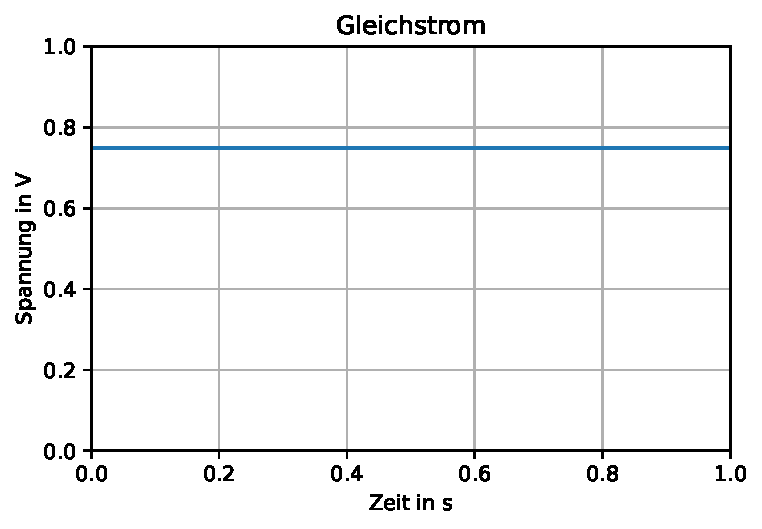
\includegraphics[keepaspectratio]{tut/tut_03_Periodische-Signale_files/figure-pdf/fig-gleichstrom-output-1.pdf}}

}

\caption{\label{fig-gleichstrom}Gleichstrom}

\end{figure}%

\begin{Shaded}
\begin{Highlighting}[]
\ImportTok{import}\NormalTok{ numpy }\ImportTok{as}\NormalTok{ np}
\ImportTok{import}\NormalTok{ matplotlib.pyplot }\ImportTok{as}\NormalTok{ plt}

\NormalTok{T }\OperatorTok{=} \DecValTok{1}
\NormalTok{fs }\OperatorTok{=} \DecValTok{1000}
\NormalTok{time }\OperatorTok{=}\NormalTok{ np.linspace (}\DecValTok{0}\NormalTok{, T, T}\OperatorTok{*}\NormalTok{fs)}

\NormalTok{f }\OperatorTok{=} \DecValTok{5}
\NormalTok{sinus1 }\OperatorTok{=}\NormalTok{ np.sin(}\DecValTok{2} \OperatorTok{*}\NormalTok{ np.pi }\OperatorTok{*}\NormalTok{ f }\OperatorTok{*}\NormalTok{ time)}
\NormalTok{sinus2 }\OperatorTok{=}\NormalTok{ np.sin(}\DecValTok{2} \OperatorTok{*}\NormalTok{ np.pi }\OperatorTok{*} \FloatTok{0.5}\OperatorTok{*}\NormalTok{f }\OperatorTok{*}\NormalTok{ time)}

\NormalTok{plt.figure()}
\NormalTok{plt.plot(time,sinus1}\OperatorTok{+}\NormalTok{sinus2)}
\NormalTok{plt.xlabel(}\StringTok{\textquotesingle{}Zeit in s\textquotesingle{}}\NormalTok{)}
\NormalTok{plt.ylabel(}\StringTok{\textquotesingle{}Spannung in V\textquotesingle{}}\NormalTok{)}
\NormalTok{plt.title(}\StringTok{\textquotesingle{}Wechselstrom\textquotesingle{}}\NormalTok{)}
\NormalTok{plt.grid()}
\NormalTok{plt.show()}
\end{Highlighting}
\end{Shaded}

\begin{figure}[H]

\centering{

\pandocbounded{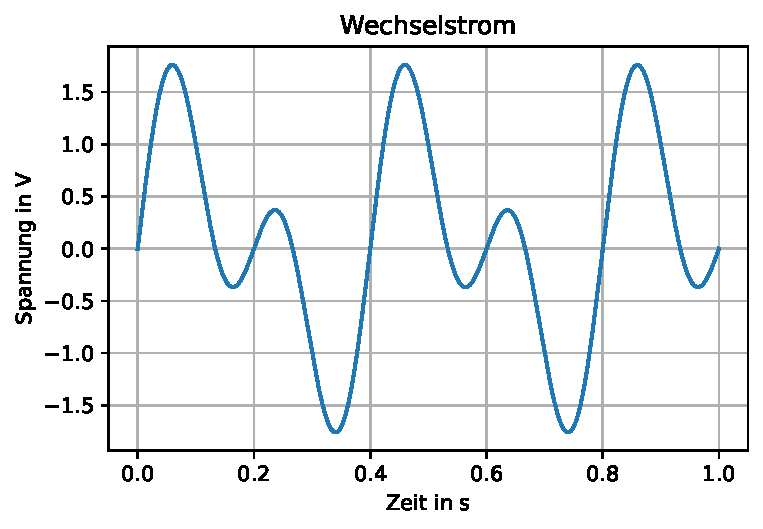
\includegraphics[keepaspectratio]{tut/tut_03_Periodische-Signale_files/figure-pdf/fig-wechselstrom-output-1.pdf}}

}

\caption{\label{fig-wechselstrom}Wechselstrom}

\end{figure}%

\begin{Shaded}
\begin{Highlighting}[]
\ImportTok{import}\NormalTok{ numpy }\ImportTok{as}\NormalTok{ np}
\ImportTok{import}\NormalTok{ matplotlib.pyplot }\ImportTok{as}\NormalTok{ plt}

\NormalTok{T }\OperatorTok{=} \DecValTok{1}
\NormalTok{fs }\OperatorTok{=} \DecValTok{1000}
\NormalTok{time }\OperatorTok{=}\NormalTok{ np.linspace (}\DecValTok{0}\NormalTok{, T, T}\OperatorTok{*}\NormalTok{fs)}

\NormalTok{f }\OperatorTok{=} \DecValTok{5}
\NormalTok{sinus }\OperatorTok{=}\NormalTok{ np.sin(}\DecValTok{2} \OperatorTok{*}\NormalTok{ np.pi }\OperatorTok{*}\NormalTok{ f }\OperatorTok{*}\NormalTok{ time)}

\NormalTok{plt.figure()}
\NormalTok{plt.plot(time,sinus)}
\NormalTok{plt.xlabel(}\StringTok{\textquotesingle{}Zeit in s\textquotesingle{}}\NormalTok{)}
\NormalTok{plt.ylabel(}\StringTok{\textquotesingle{}Spannung in V\textquotesingle{}}\NormalTok{)}
\NormalTok{plt.title(}\StringTok{\textquotesingle{}Sinusstrom\textquotesingle{}}\NormalTok{)}
\NormalTok{plt.grid()}
\NormalTok{plt.show()}
\end{Highlighting}
\end{Shaded}

\begin{figure}[H]

\centering{

\pandocbounded{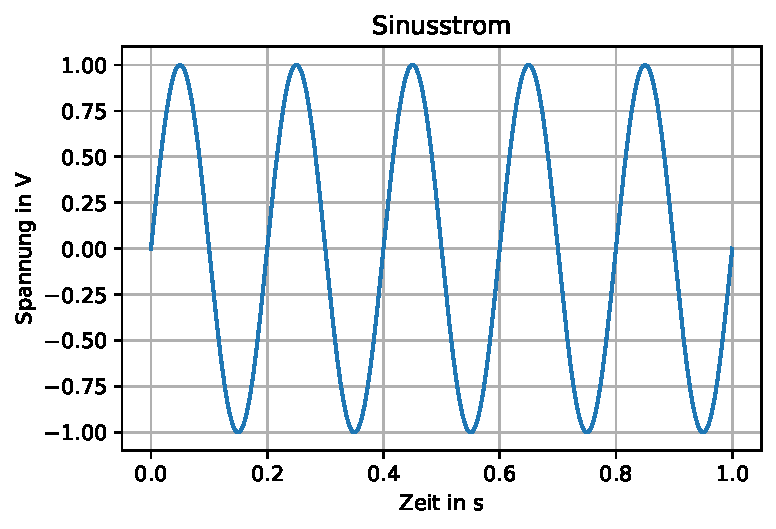
\includegraphics[keepaspectratio]{tut/tut_03_Periodische-Signale_files/figure-pdf/fig-sinusstrom-output-1.pdf}}

}

\caption{\label{fig-sinusstrom}Sinusstrom}

\end{figure}%

\begin{Shaded}
\begin{Highlighting}[]
\ImportTok{import}\NormalTok{ numpy }\ImportTok{as}\NormalTok{ np}
\ImportTok{import}\NormalTok{ matplotlib.pyplot }\ImportTok{as}\NormalTok{ plt}

\NormalTok{T }\OperatorTok{=} \DecValTok{1}
\NormalTok{fs }\OperatorTok{=} \DecValTok{1000}
\NormalTok{time }\OperatorTok{=}\NormalTok{ np.linspace (}\DecValTok{0}\NormalTok{, T, T}\OperatorTok{*}\NormalTok{fs)}

\NormalTok{f }\OperatorTok{=} \DecValTok{5}
\NormalTok{sinus }\OperatorTok{=}\NormalTok{ np.sin(}\DecValTok{2} \OperatorTok{*}\NormalTok{ np.pi }\OperatorTok{*}\NormalTok{ f }\OperatorTok{*}\NormalTok{ time)}

\NormalTok{plt.figure()}
\NormalTok{plt.plot(time,sinus}\OperatorTok{+}\FloatTok{0.5}\NormalTok{)}
\NormalTok{plt.xlabel(}\StringTok{\textquotesingle{}Zeit in s\textquotesingle{}}\NormalTok{)}
\NormalTok{plt.ylabel(}\StringTok{\textquotesingle{}Spannung in V\textquotesingle{}}\NormalTok{)}
\NormalTok{plt.title(}\StringTok{\textquotesingle{}Mischstrom\textquotesingle{}}\NormalTok{)}
\NormalTok{plt.grid()}
\NormalTok{plt.show()}
\end{Highlighting}
\end{Shaded}

\begin{figure}[H]

\centering{

\pandocbounded{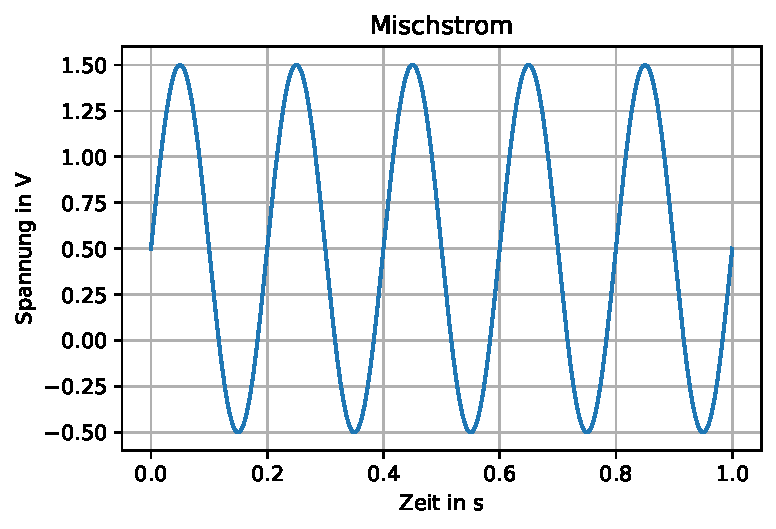
\includegraphics[keepaspectratio]{tut/tut_03_Periodische-Signale_files/figure-pdf/fig-mischstrom-output-1.pdf}}

}

\caption{\label{fig-mischstrom}Mischstrom}

\end{figure}%

\begin{Shaded}
\begin{Highlighting}[]
\ImportTok{import}\NormalTok{ numpy }\ImportTok{as}\NormalTok{ np}
\ImportTok{import}\NormalTok{ matplotlib.pyplot }\ImportTok{as}\NormalTok{ plt}

\NormalTok{T }\OperatorTok{=} \DecValTok{1}
\NormalTok{fs }\OperatorTok{=} \DecValTok{1000}
\NormalTok{time }\OperatorTok{=}\NormalTok{ np.linspace (}\DecValTok{0}\NormalTok{, T, T}\OperatorTok{*}\NormalTok{fs)}

\NormalTok{f }\OperatorTok{=} \DecValTok{20}
\NormalTok{sinus1 }\OperatorTok{=}\NormalTok{ np.sin(}\DecValTok{2} \OperatorTok{*}\NormalTok{ np.pi }\OperatorTok{*}\NormalTok{ f }\OperatorTok{*}\NormalTok{ time)}
\NormalTok{sinus2 }\OperatorTok{=} \FloatTok{0.2} \OperatorTok{*}\NormalTok{ np.sin(}\DecValTok{2} \OperatorTok{*}\NormalTok{ np.pi }\OperatorTok{*} \FloatTok{0.1}\OperatorTok{*}\NormalTok{f }\OperatorTok{*}\NormalTok{ time)}
\NormalTok{modulated }\OperatorTok{=}\NormalTok{ (}\DecValTok{1} \OperatorTok{+} \FloatTok{0.5} \OperatorTok{*}\NormalTok{ np.sin(}\DecValTok{2} \OperatorTok{*}\NormalTok{ np.pi }\OperatorTok{*} \FloatTok{0.1}\OperatorTok{*}\NormalTok{f }\OperatorTok{*}\NormalTok{ time)) }\OperatorTok{*}\NormalTok{ np.sin(}\DecValTok{2} \OperatorTok{*}\NormalTok{ np.pi }\OperatorTok{*}\NormalTok{ f }\OperatorTok{*}\NormalTok{ time)}

\NormalTok{plt.figure()}
\NormalTok{plt.plot(time,modulated)}
\NormalTok{plt.xlabel(}\StringTok{\textquotesingle{}Zeit in s\textquotesingle{}}\NormalTok{)}
\NormalTok{plt.ylabel(}\StringTok{\textquotesingle{}Spannung in V\textquotesingle{}}\NormalTok{)}
\NormalTok{plt.title(}\StringTok{\textquotesingle{}amplituden{-}moduliertes Signal\textquotesingle{}}\NormalTok{)}
\NormalTok{plt.grid()}
\NormalTok{plt.show()}
\end{Highlighting}
\end{Shaded}

\begin{figure}[H]

\centering{

\pandocbounded{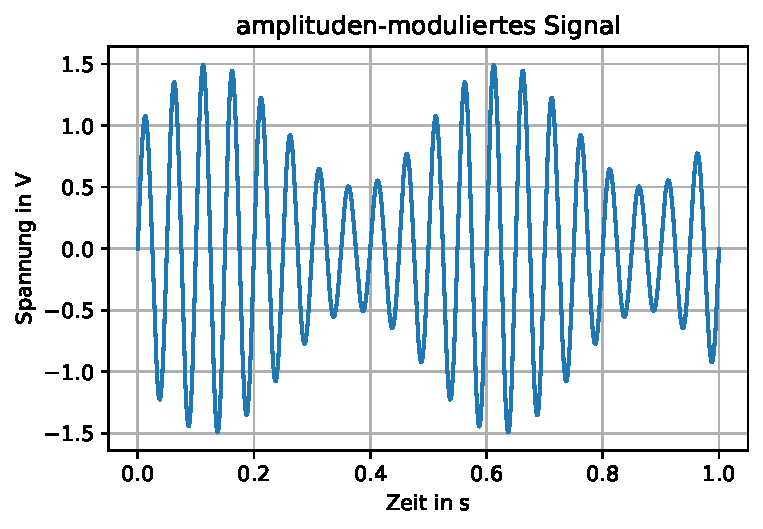
\includegraphics[keepaspectratio]{tut/tut_03_Periodische-Signale_files/figure-pdf/fig-amplitudenmodu-output-1.pdf}}

}

\caption{\label{fig-amplitudenmodu}Amplituden-moduliertes Signal}

\end{figure}%

\begin{Shaded}
\begin{Highlighting}[]
\ImportTok{import}\NormalTok{ numpy }\ImportTok{as}\NormalTok{ np}
\ImportTok{import}\NormalTok{ matplotlib.pyplot }\ImportTok{as}\NormalTok{ plt}

\NormalTok{fs }\OperatorTok{=} \DecValTok{2000}
\NormalTok{fc }\OperatorTok{=} \DecValTok{100}
\NormalTok{fm }\OperatorTok{=} \DecValTok{15}
\NormalTok{beta }\OperatorTok{=} \DecValTok{3}
\NormalTok{t }\OperatorTok{=}\NormalTok{ np.arange(}\DecValTok{0}\NormalTok{,}\FloatTok{0.2}\NormalTok{,}\DecValTok{1}\OperatorTok{/}\NormalTok{fs)}

\NormalTok{frm }\OperatorTok{=}\NormalTok{ np.cos(}\DecValTok{2}\OperatorTok{*}\NormalTok{np.pi}\OperatorTok{*}\NormalTok{fc}\OperatorTok{*}\NormalTok{t }\OperatorTok{+}\NormalTok{ beta}\OperatorTok{*}\NormalTok{np.sin(}\DecValTok{2}\OperatorTok{*}\NormalTok{np.pi}\OperatorTok{*}\NormalTok{fm}\OperatorTok{*}\NormalTok{t))}
\NormalTok{m }\OperatorTok{=}\NormalTok{ np.cos(}\DecValTok{2}\OperatorTok{*}\NormalTok{np.pi}\OperatorTok{*}\NormalTok{fm}\OperatorTok{*}\NormalTok{t)}

\NormalTok{plt.figure()}
\NormalTok{plt.plot(t,frm)}
\NormalTok{plt.xlabel(}\StringTok{\textquotesingle{}Zeit in s\textquotesingle{}}\NormalTok{)}
\NormalTok{plt.ylabel(}\StringTok{\textquotesingle{}Spannung in V\textquotesingle{}}\NormalTok{)}
\NormalTok{plt.title(}\StringTok{\textquotesingle{}frequenz{-}moduliertes Signal\textquotesingle{}}\NormalTok{)}
\NormalTok{plt.grid()}
\NormalTok{plt.show()}
\end{Highlighting}
\end{Shaded}

\begin{figure}[H]

\centering{

\pandocbounded{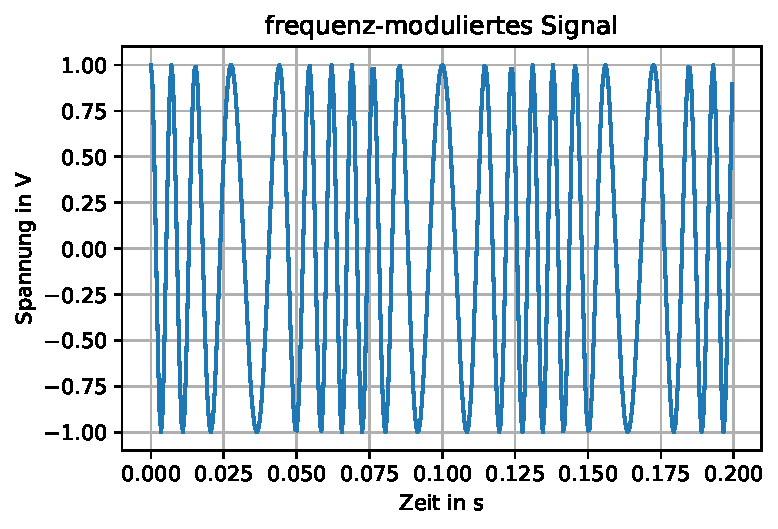
\includegraphics[keepaspectratio]{tut/tut_03_Periodische-Signale_files/figure-pdf/fig-frequenzmodu-output-1.pdf}}

}

\caption{\label{fig-frequenzmodu}Frequenz-moduliertes Signal}

\end{figure}%

\section{Kennwerte von
Wechselgrößen}\label{kennwerte-von-wechselgruxf6uxdfen}

Allgemein kann man eine sich zeitlich ändernde sinusförmige Wechselgröße
mit der folgenden Funktion beschreiben.

\[
x = \hat{x} sin(\omega t + \varphi)
\]

Dabei wird der Zeitwert x als auch der Scheitelwert \(\hat{x}\) mit
einem kleinen Formelbuchstaben bezeichnet.

\subsection{Periodendauer und
Frequenz}\label{periodendauer-und-frequenz}

Da sich eine sinusförmige Wechselgröße wiederholt sich nach Ablauf des
Winkels \(2\pi = 360^° = \omega T\). Damit kann man die Periodendauer T
über die Kreisfrequenz \(\omega\) darstellen.

\[
T = \frac{2 \pi}{\omega}
\]

Die Frequenz f gibt die Anzahl der Perioden pro Sekunde an und wird in
Hz = 1/s gemessen. Die Frequenz ist der Kehrwert der Periodendauer.

\[
f = \frac{1}{T}
\]

Die Kreisfreqeunz ist die Frequenz mit dem Faktor \(2\pi\) erweitert.
Sie wird in 1/s und \textbf{nicht} in Hz gemessen!

\[
\omega = 2 \pi f = \frac{2\pi}{T}
\]

\subsection{Phasenlage}\label{phasenlage}

Sinusgrößen können zu verschiedenen Zeitpunkten ihre Scheitelwerte und
Nulldurchgänge erreichen. Man sagt, dass diese Größen unterschiedliche
Phasenlagen haben; sie sind gegeneinander phasenverschoben.

\begin{figure}

\centering{

\includegraphics[width=4.16667in,height=\textheight,keepaspectratio]{tut/../images/tut/chap3/Phasenlage.pdf}

}

\caption{\label{fig-TutChapPhasenlage}Phasenlage}

\end{figure}%

Entn. aus (Fricke und Vaske 1982)

\subsubsection{Nullphasenwinkel}\label{nullphasenwinkel}

Allgemein gesprochen beginnt eine Sinusfunktion bei t=0 und geht um den
Nullphasenwinkel \(\varphi_x\) früher als die normale Sinusfunktion
\(sin(\omega t)\) durch Null. Das Vorzeichen des Winkel ist sehr
wichtig!

Beim positiven Nulldurchgang der Sinusgröße wird ein Pfeil zum Nullpunkt
gezeichnet. Ist der Pfeil in Zählrichtung der Zeitachse ist der
Nullphasenwinkel positiv, ist der Pfeil entgegen der Zählrichtung der
Zeitachse, dann ist er negativ (siehe Bild unter Phasenlage).

\subsubsection{Phasenwinkel}\label{phasenwinkel}

Zusätzlich zum Nullphasewinkel gibt es den Phasenwinkel. Dieser gibt die
Phasenverschiebung zwischen zwei Sinussignalen an. Es ist festgelegt,
dass der Strom in solchen Fällen als Bezugsgröße genommen wird.

\[
\varphi = \varphi_U - \varphi_I
\]

Beispiel:

\[
\varphi_I = -\frac{\pi}{3} = -60°
\]

\[
\varphi_U = \frac{\pi}{6} = 30°
\]

\[
\varphi = \varphi_U - \varphi_I = \left( \frac{\pi}{6} \right) - \left( -\frac{\pi}{3} \right) = 30° - (-60°) = \frac{\pi}{2} = 90°
\]

Die Spannung eilt dem Strom um \(\varphi = 90°\) vor.

\subsection{Mittelwert}\label{mittelwert-1}

Der Mittelwert ist der zeitlich durchschnittliche Wert einer Funktion.

\[
\overline{x(t)} = \frac{1}{T} \int\limits_{t_0}^{t_o + T} x(t) dt
\]

Bei reinem Wechselstrom ist der Mittelwert 0.

\subsection{Gleichrichtwert}\label{gleichrichtwert}

Der Gleichrichtwert ist der Mittelwert einer gleichgericheten Größe.

\[
\overline{|x(t)|} = \frac{1}{T} \int\limits_{t_0}^{t_0 + T} |x(t)| dt
\]

Verhältnis von Gleichricht- zu Scheitelwert (bei Sinusgrößen):
\(\frac{\overline{|i|}}{\hat{i}} = 0.6366\)

\subsection{Effektivwert}\label{effektivwert-1}

Der Effektivwert einer periodischen Spannung (oder eines periodischen
Stroms) entspricht dem Wert einer Gleichspannung (eines Gleichstroms),
der in einer ohmschen Last dieselbe Leistung umsetzt.

\[
X = X_{eff} = \sqrt{\frac{1}{T} \int\limits_{t_0}^{t_0 + T} x^2(t) dt}
\]

\textbf{Scheitelfaktor}

Der Scheitelfaktor ist das Verhältnis von Scheitelwert \(\hat{i}\) bzw.
\(\hat{u}\) zum Effektivwert I bzw. U.

\[
\xi = \frac{\hat{x}}{X_{eff}}
\]

Der Scheitelfaktor für Sinusgrößen beträgt \(\xi = \sqrt{2} = 1.414\).

Der Scheitelfaktor für Dreieckspannung beträgt \(\xi = \sqrt{3}\).

Der Scheitelfaktor für Rechtecksignale beträgt \(\xi = 1\).

\textbf{Formfaktor}

Der Formfaktor stellt das Verhältnis von Effektivwert I bzw. U zu
Gleichrichtwert \(\overline{|i|}\) bzw. \(\overline{|u|}\) dar.

\[
F = \frac{X_{eff}}{\overline{|x|}}
\]

Der Formfaktor für Sinusgrößen beträgt
\(F = \frac{\pi}{2\sqrt{2}} \approx 1.11\).

Der Formfaktor für Dreiecksignale beträgt \(F = \frac{1.11}{2}\).

Der Formfaktor für Rechtecksignale beträgt \(F = 1.11\).

\subsection{Effektivwert mit
Gleichstromanteil}\label{effektivwert-mit-gleichstromanteil}

\begin{figure}

\centering{

\pandocbounded{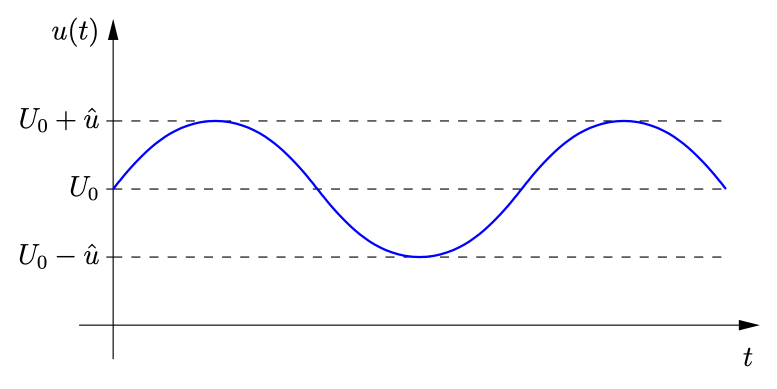
\includegraphics[keepaspectratio]{tut/../images/tut/chap3/Mischspannung.pdf}}

}

\caption{\label{fig-TutChapMischspannung}Mischspannung}

\end{figure}%

Entn. aus (Schenke 2023)

\[
X_{eff} = \sqrt{X_o^2 + X_{eff\sim}^2}
\]

\section{Übungen}\label{uxfcbungen-1}

\subsection{Aufgabe Gleichrichtwert}\label{aufgabe-gleichrichtwert}

Ein Sinusstrom mit dem Scheitelwert \(\hat{i} = 10 A\) fließt durch die
Gleichrichterschaltung-Brückenschaltung von Bild 3.4.

\begin{figure}

\centering{

\pandocbounded{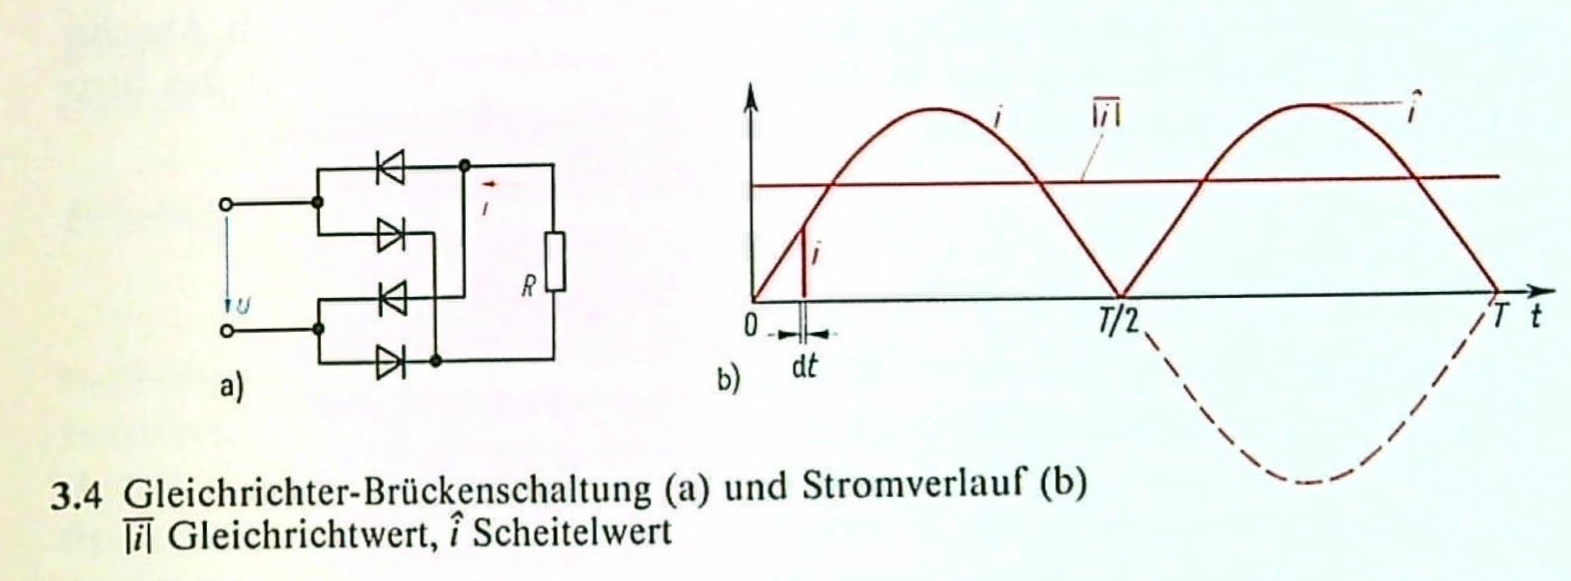
\includegraphics[keepaspectratio]{tut/../images/tut/chap3/Brueckengleichrichter.pdf}}

}

\caption{\label{fig-TutChapAufg3.1}Aufgabe 3.1}

\end{figure}%

Entn. aus (Fricke und Vaske 1982)

Welche Elektrizitätsmenge Q wird während der Zeit t = 2 h befördert?\\
Tipp: \(Q = i \cdot t\)

\begin{tcolorbox}[enhanced jigsaw, arc=.35mm, opacityback=0, opacitybacktitle=0.6, left=2mm, breakable, title=\textcolor{quarto-callout-caution-color}{\faFire}\hspace{0.5em}{Lösung}, bottomrule=.15mm, toptitle=1mm, rightrule=.15mm, titlerule=0mm, leftrule=.75mm, colframe=quarto-callout-caution-color-frame, colbacktitle=quarto-callout-caution-color!10!white, bottomtitle=1mm, colback=white, toprule=.15mm, coltitle=black]

\[
\overline{|i|} = 0.6366 \hat{i} = 0.6366 \cdot 10 A = 6.366 A
\]

\[
Q = \overline{|i|} t = 6.366 A \cdot 2 h = 12.73 Ah
\]

\end{tcolorbox}

\subsection{Aufgabe Zeitfunktion
berechnen}\label{aufgabe-zeitfunktion-berechnen}

Die übliche Netzspannung 1982 betrug \(U = 220 V\) bei der Netzfrequenz
\(f = 50 Hz\). Es sind der Gleichrichtwert \(\overline{|u|}\) und die
Zeitfunktion u dieser Spannung zu bestimmen.

\begin{tcolorbox}[enhanced jigsaw, arc=.35mm, opacityback=0, opacitybacktitle=0.6, left=2mm, breakable, title=\textcolor{quarto-callout-caution-color}{\faFire}\hspace{0.5em}{Lösung}, bottomrule=.15mm, toptitle=1mm, rightrule=.15mm, titlerule=0mm, leftrule=.75mm, colframe=quarto-callout-caution-color-frame, colbacktitle=quarto-callout-caution-color!10!white, bottomtitle=1mm, colback=white, toprule=.15mm, coltitle=black]

Netzspannung ist Sinusförmig --\textgreater{} Formfaktor F = 1.111

Gleichrichtwert:

\[
\overline{|u|} = \frac{U}{F} = \frac{220 V}{1.111} = 198 V
\]

Zeitfunktion:

Scheitelwert:

\[
\hat{u} = \sqrt{2} U = \sqrt{2} \cdot 220 V = 311.1 V
\]

Kreisfrequenz:

\[
\omega = 2 \pi f = 2 \pi \cdot 50 Hz = 314.2 \frac{1}{s}
\]

\[
u = \hat{u} sin(\omega t) = 311.1 V \cdot sin(314.2 1/s)
\]

\end{tcolorbox}

\subsection{Aufgabe Mittelwerte aus Zeitverlauf
bestimmen}\label{aufgabe-mittelwerte-aus-zeitverlauf-bestimmen}

\begin{figure}

\centering{

\pandocbounded{\includegraphics[keepaspectratio]{tut/../images/tut/chap3/Aufgabe2.3.pdf}}

}

\caption{\label{fig-TutChap3Aufg3.3}Aufgabe 3.3}

\end{figure}%

Entn. aus (Albach und Fischer 2020)

\begin{tcolorbox}[enhanced jigsaw, arc=.35mm, opacityback=0, opacitybacktitle=0.6, left=2mm, breakable, title=\textcolor{quarto-callout-caution-color}{\faFire}\hspace{0.5em}{Lösung 3.3}, bottomrule=.15mm, toptitle=1mm, rightrule=.15mm, titlerule=0mm, leftrule=.75mm, colframe=quarto-callout-caution-color-frame, colbacktitle=quarto-callout-caution-color!10!white, bottomtitle=1mm, colback=white, toprule=.15mm, coltitle=black]

\begin{enumerate}
\def\labelenumi{\alph{enumi})}
\tightlist
\item
  Mittelwert:
\end{enumerate}

\[
\overline{u} = \frac{1}{T} \int\limits_{0}^{T} u(t)dt = \frac{1}{T} \left[ \hat{u} \frac{3T}{4} - \hat{u} \frac{T}{4}
\right] = \frac{\hat{u}}{2} = 5 V
\]

Gleichrichtwert:

\[
\overline{|u|} = \frac{1}{T} \int\limits_{0}^{T} |u(t)|dt = \frac{1}{T} \left[ \hat{u} \frac{3T}{4} + |-\hat{u}|
\frac{T}{4} \right] = \hat{u} = 10 V
\]

Effektivwert:

\[
U_{eff} = \sqrt{\frac{1}{T} \int\limits_{0}^{T} u^2(t)dt} = \sqrt{\frac{1}{T} \left[ \hat{u}^2 \frac{3T}{4} +
(-\hat{u}^2) \frac{T}{4} \right]} = \hat{u} = 10 V
\]

\begin{enumerate}
\def\labelenumi{\alph{enumi})}
\setcounter{enumi}{1}
\tightlist
\item
  Mittelwert:
\end{enumerate}

\[
\overline{u} = \frac{1}{T} \int\limits_{0}^{T} \hat{u} \frac{t}{T} dt = \frac{\hat{u}}{T^2} \frac{t^2}{2} \Big\vert_0^T
= \frac{\hat{u}}{2} = 5 V
\]

Gleichrichtwert:

\[
\overline{|u|} = |u| = 5 V
\]

Effektivwert:

\[
U_{eff} = \sqrt{\frac{1}{T} \int\limits_{0}^{T} \left(\hat{u} \frac{t}{T} \right)^2 dt} 
= \sqrt{\frac{\hat{u}^2}{T^3} \frac{t^3}{3} \Big\vert_0^T} = \sqrt{\frac{\hat{u}^2}{3}} 
= \frac{\hat{u}}{\sqrt{3}} = 5.77 V
\]

\begin{enumerate}
\def\labelenumi{\alph{enumi})}
\setcounter{enumi}{2}
\tightlist
\item
  Mittelwert:
\end{enumerate}

\[
\overline{u} = \frac{\hat{u}}{4} = 2.5 V
\]

Gleichrichtwert:

\[
\overline{|u|} = \overline{u} = 2.5 V
\]

Effektivwert:

\[
U_{eff} = \sqrt{\frac{1}{T} \int\limits_{0}^{T/2} \left(2\hat{u} \frac{t}{T} \right)^2 dt} 
= \sqrt{\frac{4\hat{u}^2}{T^3} \frac{t^3}{3} \Big\vert_0^{T/2}} 
= \sqrt{\frac{\hat{u}^2}{6}} 
= \frac{\hat{u}}{\sqrt{6}} = 4.08 V
\]

\begin{enumerate}
\def\labelenumi{\alph{enumi})}
\setcounter{enumi}{3}
\tightlist
\item
  Mittelwert:
\end{enumerate}

\[
\overline{u} = 0 V
\]

Gleichrichtwert:

\[
\overline{|u|} = \frac{1}{T} \left[ \hat{u} \frac{T}{4} + \hat{u} \frac{T}{4} \right] = \frac{\hat{u}}{2} = 5 V
\]

Effektivwert:

\[
U_{eff} = \sqrt{\frac{1}{T} \int\limits_{0}^{T/2} \left( 2\hat{u} \frac{t}{T} \right)^2 dt + \frac{1}{T} \int\limits_{T/2}^{T} \left( 2\hat{u} \frac{t - T}{T} \right)^2 dt} = \sqrt{\frac{\hat{u}^2}{6} + \frac{\hat{u}^2}{6}} = \frac{\hat{u}}{\sqrt{3}} = 5.77 V
\]

\end{tcolorbox}

\subsection{Aufgabe 3.4}\label{aufgabe-3.4}

Ein Wechselstrom besteht nach der Abbildung aus ``angeschnittenen''
Sinushalbschwingungen. In den Bereichen \(0 < \omega t
< \alpha\) und \(\pi < \omega t < (\pi + \alpha)\) fließt kein Strom (i
= 0), wobei \(\alpha = \pi/4 = 45°\) sei. In der übrigen Zeit (innerhalb
des Bereiches \(0 < \omega t < 2\pi)\) wird der Stromverlauf durch die
Gleichung \(i = \hat{i}
sin(\omega t)\) wiedergegeben. Hierbei betrage der Scheitelwert des
Stromes \(\hat{i} = 10 A\).

Wie groß ist der Effektivwert I des Stromes?

\begin{Shaded}
\begin{Highlighting}[]
\ImportTok{import}\NormalTok{ numpy }\ImportTok{as}\NormalTok{ np}
\ImportTok{import}\NormalTok{ matplotlib.pyplot }\ImportTok{as}\NormalTok{ plt}

\NormalTok{omega\_t }\OperatorTok{=}\NormalTok{ np.arange(}\DecValTok{0}\NormalTok{,}\DecValTok{2}\OperatorTok{*}\NormalTok{np.pi,np.pi}\OperatorTok{/}\NormalTok{(}\DecValTok{2}\OperatorTok{**}\DecValTok{6}\NormalTok{))}
\NormalTok{i }\OperatorTok{=} \DecValTok{10} \OperatorTok{*}\NormalTok{ np.sin(omega\_t)}

\NormalTok{alpha }\OperatorTok{=}\NormalTok{ np.pi}\OperatorTok{/}\DecValTok{4}

\ControlFlowTok{for}\NormalTok{ a }\KeywordTok{in} \BuiltInTok{range}\NormalTok{(}\BuiltInTok{len}\NormalTok{(i)):}
    \ControlFlowTok{if}\NormalTok{ omega\_t[a] }\OperatorTok{\textless{}}\NormalTok{ alpha }\KeywordTok{or}\NormalTok{ (omega\_t[a] }\OperatorTok{\textgreater{}}\NormalTok{ np.pi }\KeywordTok{and}\NormalTok{ omega\_t[a] }\OperatorTok{\textless{}}\NormalTok{ np.pi}\OperatorTok{+}\NormalTok{alpha):}
\NormalTok{        i[a] }\OperatorTok{=} \DecValTok{0}
        
\NormalTok{list\_ticks }\OperatorTok{=}\NormalTok{ [}\VariableTok{None}\NormalTok{]}\OperatorTok{*}\DecValTok{128}
\NormalTok{list\_ticks[}\DecValTok{0}\NormalTok{] }\OperatorTok{=} \StringTok{\textquotesingle{}0\textquotesingle{}}
\NormalTok{list\_ticks[}\DecValTok{63}\NormalTok{] }\OperatorTok{=} \StringTok{\textquotesingle{}$}\ErrorTok{\textbackslash{}}\StringTok{pi$\textquotesingle{}}
\NormalTok{list\_ticks[}\DecValTok{127}\NormalTok{] }\OperatorTok{=} \StringTok{\textquotesingle{}$2}\ErrorTok{\textbackslash{}}\StringTok{pi$\textquotesingle{}}
        
\NormalTok{plt.figure()}
\NormalTok{plt.plot(omega\_t, i)}
\NormalTok{plt.xlabel(}\StringTok{\textquotesingle{}$}\ErrorTok{\textbackslash{}}\StringTok{omega t$\textquotesingle{}}\NormalTok{)}
\NormalTok{plt.ylabel(}\StringTok{\textquotesingle{}i\textquotesingle{}}\NormalTok{)}
\CommentTok{\#plt.xticks([0,63,127],[\textquotesingle{}0\textquotesingle{},\textquotesingle{}$\textbackslash{}pi$\textquotesingle{},\textquotesingle{}2$\textbackslash{}pi$\textquotesingle{}])}
\NormalTok{plt.xticks(omega\_t,list\_ticks)}
\NormalTok{plt.grid(}\VariableTok{True}\NormalTok{)}
\end{Highlighting}
\end{Shaded}

\begin{figure}[H]

\centering{

\pandocbounded{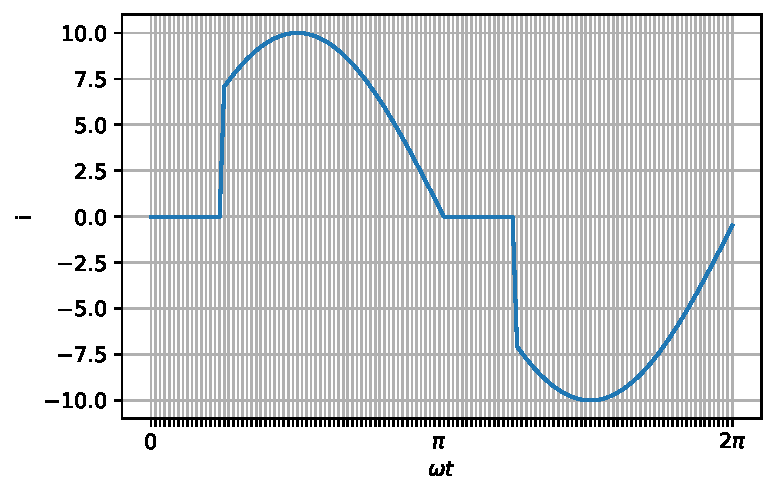
\includegraphics[keepaspectratio]{tut/tut_03_Periodische-Signale_files/figure-pdf/fig-aufg3.4-output-1.pdf}}

}

\caption{\label{fig-aufg3.4}Aufgabe 3.4}

\end{figure}%

\begin{tcolorbox}[enhanced jigsaw, arc=.35mm, opacityback=0, opacitybacktitle=0.6, left=2mm, breakable, title=\textcolor{quarto-callout-caution-color}{\faFire}\hspace{0.5em}{Lösung}, bottomrule=.15mm, toptitle=1mm, rightrule=.15mm, titlerule=0mm, leftrule=.75mm, colframe=quarto-callout-caution-color-frame, colbacktitle=quarto-callout-caution-color!10!white, bottomtitle=1mm, colback=white, toprule=.15mm, coltitle=black]

\[
I = \sqrt{\frac{1}{2\pi} \int\limits_{0}^{2\pi} i^2 d\omega t}
\]

\[
\int\limits_{0}^{2\pi} i^2 d\omega t = 2\int\limits_{0}^{\pi} i^2 d\omega t = 2\int\limits_{0}^{\pi} \hat{i}^2 \cdot sin^2(\omega t) d\omega t
\]

\[
2\int\limits_{0}^{\pi} \hat{i}^2 \cdot sin^2(\omega t) d\omega t = 2\hat{i}^2 \left(\frac{1}{2} \omega t - \frac{1}{4} sin(2\omega t) \right) \Big\vert_\alpha^\pi = \hat{i}^2 \left( \pi - \alpha + \frac{1}{2} sin(2\alpha) \right)
\]

\[
I = \sqrt{\frac{1}{2\pi} \cdot \int\limits_{0}^{2\pi} i^2 d\omega t} = \sqrt{\frac{1}{2\pi} \hat{i}^2 \left( \pi - \alpha + \frac{1}{2} sin(2\alpha) \right)} = \sqrt{\frac{1}{2\pi} \cdot (10 A)^2 \cdot \left( \pi - \frac{\pi}{4} + \frac{1}{2} \cdot sin(2 \cdot 45°) \right)} = 6.74 A
\]

\end{tcolorbox}

\subsection{Aufgabe 3.5}\label{aufgabe-3.5}

An einem ohmschen Widerstand \(R = 30 \Omega\) liegt eine
mittelwertfreie Dreieckspannung mit der Amplitude \(\hat{u} = 9
V\) und der Frequenz \(f = 100 Hz\) an.

Welche Wirkleistung P wird im zeitlichen Mittel im Widerstand R
umgesetzt?

\begin{tcolorbox}[enhanced jigsaw, arc=.35mm, opacityback=0, opacitybacktitle=0.6, left=2mm, breakable, title=\textcolor{quarto-callout-caution-color}{\faFire}\hspace{0.5em}{Lösung}, bottomrule=.15mm, toptitle=1mm, rightrule=.15mm, titlerule=0mm, leftrule=.75mm, colframe=quarto-callout-caution-color-frame, colbacktitle=quarto-callout-caution-color!10!white, bottomtitle=1mm, colback=white, toprule=.15mm, coltitle=black]

Dreieckspannung --\textgreater{} Scheitelfaktor \(\xi = \sqrt{3}\)

\[
U = \frac{\hat{u}}{\sqrt{3}} = \frac{9 V}{\sqrt{3}} = 5.196 V
\]

\[
P = \frac{U^2}{R} = \frac{5.196 V}{30 \Omega} = 0.9 W
\]

\end{tcolorbox}

\subsection{Aufgabe 3.6}\label{aufgabe-3.6}

An einem ohmschen Widerstand R liegt eine Zägezahnspannung, die von
einer Gleichspannung überlagert ist, an:

\begin{figure}

\centering{

\pandocbounded{\includegraphics[keepaspectratio]{tut/../images/tut/chap3/Aufgabe2.6.pdf}}

}

\caption{\label{fig-TutChap3Aufg3.6}Aufgabe 3.6}

\end{figure}%

Entn. aus (Schenke 2023)

\begin{enumerate}
\def\labelenumi{\alph{enumi})}
\item
  Bestimmen Sie den Mittelwert \(\overline{u(t)}\) des periodischen
  Spannungsverlaufes u(t).
\item
  Berechnen Sie den Effektivwert U des periodischen Spannungsverlaufes
  u(t).
\item
  Welche Wirkleistung P wird im zeitlichen Mittel im Widerstand R
  umgesetzt? (23.4)
\end{enumerate}

\begin{tcolorbox}[enhanced jigsaw, arc=.35mm, opacityback=0, opacitybacktitle=0.6, left=2mm, breakable, title=\textcolor{quarto-callout-caution-color}{\faFire}\hspace{0.5em}{Lösung}, bottomrule=.15mm, toptitle=1mm, rightrule=.15mm, titlerule=0mm, leftrule=.75mm, colframe=quarto-callout-caution-color-frame, colbacktitle=quarto-callout-caution-color!10!white, bottomtitle=1mm, colback=white, toprule=.15mm, coltitle=black]

\begin{enumerate}
\def\labelenumi{\alph{enumi})}
\tightlist
\item
\end{enumerate}

\[
\overline{u(t)} = \frac{U_1 + U_2}{2}
\]

\begin{enumerate}
\def\labelenumi{\alph{enumi})}
\setcounter{enumi}{1}
\tightlist
\item
\end{enumerate}

\[
U = \sqrt{\left( \frac{U_2 - U_1}{2 \cdot \sqrt{3}} \right)^2 + \left( \frac{U_1 + U_2}{2} \right)^2}
\]

\begin{enumerate}
\def\labelenumi{\alph{enumi})}
\setcounter{enumi}{2}
\tightlist
\item
\end{enumerate}

\[
P = \frac{U^2}{R}
\]

\end{tcolorbox}

\subsection{Aufgabe 3.7}\label{aufgabe-3.7}

Durch den ohmschen Widerstand R fließt ein Sinusstrom, der mit einem
Gleichstrom überlagert ist:

\begin{figure}

\centering{

\pandocbounded{\includegraphics[keepaspectratio]{tut/../images/tut/chap3/Aufgabe2.7.pdf}}

}

\caption{\label{fig-TutChap3Aufg3.7}Aufgabe 3.7}

\end{figure}%

Entn. aus (Schenke 2023)

\begin{enumerate}
\def\labelenumi{\alph{enumi})}
\item
  Bestimmen Sie den Mittelwert \(\overline{i(t)}\) des periodischen
  Stromverlaufes i(t).
\item
  Berechnen Sie den Effektivwert I des periodischen Stromverlaufes i(t).
\item
  Welche Wirkleistung P wird im zeitlichen Mittel im Widerstand R
  umgesetzt? (23.6)
\end{enumerate}

\begin{tcolorbox}[enhanced jigsaw, arc=.35mm, opacityback=0, opacitybacktitle=0.6, left=2mm, breakable, title=\textcolor{quarto-callout-caution-color}{\faFire}\hspace{0.5em}{Lösung}, bottomrule=.15mm, toptitle=1mm, rightrule=.15mm, titlerule=0mm, leftrule=.75mm, colframe=quarto-callout-caution-color-frame, colbacktitle=quarto-callout-caution-color!10!white, bottomtitle=1mm, colback=white, toprule=.15mm, coltitle=black]

\begin{enumerate}
\def\labelenumi{\alph{enumi})}
\tightlist
\item
\end{enumerate}

\[
\overline{i(t)} = I_0
\]

\begin{enumerate}
\def\labelenumi{\alph{enumi})}
\setcounter{enumi}{1}
\tightlist
\item
\end{enumerate}

\[
I = \sqrt{I_0^2 + \left( \frac{I_0}{\sqrt{2}} \right)^2}
\]

\begin{enumerate}
\def\labelenumi{\alph{enumi})}
\setcounter{enumi}{2}
\tightlist
\item
\end{enumerate}

\[
P = I^2 \cdot R
\]

\end{tcolorbox}

\bookmarksetup{startatroot}

\chapter*{Bibliography}\label{bibliography}
\addcontentsline{toc}{chapter}{Bibliography}

\markboth{Bibliography}{Bibliography}

\phantomsection\label{refs}
\begin{CSLReferences}{1}{0}
\bibitem[\citeproctext]{ref-albach2020a}
Albach, Manfred, und Janina Fischer. 2020. \emph{Elektrotechnik
Aufgabensammlung}. Pearson.
\url{https://elibrary.pearson.de/book/99.150005/9783863268930}.

\bibitem[\citeproctext]{ref-buettner2014}
Büttner, Wolf-Ewald. 2014. \emph{Grundlagen der Elektrotechnik 2}.
{OLDENBOURG} {WISSENSCHAFTSVERLAG}.
\url{https://doi.org/10.1524/9783110371796}.

\bibitem[\citeproctext]{ref-deliyannis1998}
Deliyannis, T., Yichuang Sun, und J. K. Fidler. 1998.
\emph{Continuous-Time Active Filter Design}. CRC Press.
\url{https://doi.org/10.1201/9781439821879}.

\bibitem[\citeproctext]{ref-Fricke1982}
Fricke, H., und P. Vaske. 1982. \emph{Elektrische Netzwerke Grundlagen
der Elektrotechnik 1}. 17. Aufl. Stuttgart, Germany: B.G. Teubner.

\bibitem[\citeproctext]{ref-harriehausen2020}
Harriehausen, Thomas, und Dieter Schwarzenau. 2020. \emph{Moeller
Grundlagen der Elektrotechnik}. Springer Fachmedien Wiesbaden.
\url{https://doi.org/10.1007/978-3-658-27840-3}.

\bibitem[\citeproctext]{ref-hewlett1942}
Hewlett, W. R. 1942. {„Variable Frequency Oscillation Generator``}. U.S.
Patent Office No. 2,268,872.
\url{https://de.wikipedia.org/wiki/Wien-Robinson-Brücke}.

\bibitem[\citeproctext]{ref-kasper2000}
Kasper, Manfred. 2000. \emph{Mikrosystementwurf}. Berlin, Germany:
Springer.

\bibitem[\citeproctext]{ref-marinescu2016}
Marinescu, Marlene, und Nicolae Marinescu. 2016. \emph{Elektrotechnik
f{ü}r Studium und Praxis}. Springer Fachmedien Wiesbaden.
\url{https://doi.org/10.1007/978-3-658-14159-2}.

\bibitem[\citeproctext]{ref-mietke2024}
Mietke, Detlef. 2024. {„Elektroniktutor``}. Techreport.
Oberstufenzentrum f{ü}r Kommunikations-, Informations- und Medientechnik
(OSZ-KIM), Berlin; online. \url{https://www.elektroniktutor.de}.

\bibitem[\citeproctext]{ref-natt2020}
Natt, Oliver. 2020. \emph{Physik mit Python}. Springer Berlin
Heidelberg. \url{https://doi.org/10.1007/978-3-662-61274-3}.

\bibitem[\citeproctext]{ref-paul2019}
Paul, Steffen, und Reinhold Paul. 2019. \emph{Grundlagen der
Elektrotechnik und Elektronik 2}. Springer Berlin Heidelberg.
\url{https://doi.org/10.1007/978-3-662-58221-3}.

\bibitem[\citeproctext]{ref-reisch2007}
Reisch, Michael. 2007. \emph{Elektronische Bauelemente: Funktion,
Grundschaltungen, Modellierung mit SPICE}. 2. Aufl. Springer.
\url{https://doi.org/10.1007/978-3-540-34015-7}.

\bibitem[\citeproctext]{ref-schenke2023}
Schenke, Stefan. 2023. {„{G}rundlagen der {E}lektrotechnik --- {J}etzt
schaffst {D}u die {P}rüfung!``} Helmut-Schmidt Universit{ä}t Hamburg,
Germany; online. \url{http://www.stefan-schenke.de/get/}.

\bibitem[\citeproctext]{ref-wicht2024}
Wicht, Bernhard. 2024. \emph{Design of Power Management Integrated
Circuits}. Wiley. \url{https://doi.org/10.1002/9781119123095}.

\bibitem[\citeproctext]{ref-wikipedia2019a}
Wikipedia. 2019. {„{W}ien-{R}obinson-{B}rücke --- {W}ikipedia{,} die
freie {E}nzyklopädie``}.
\url{https://de.wikipedia.org/w/index.php?title=Wien-Robinson-Br\%C3\%BCcke&oldid=194933790}.

\bibitem[\citeproctext]{ref-wikipedia2021a}
---------. 2021. {„{B}ode-{D}iagramm --- {W}ikipedia{,} die freie
{E}nzyklopädie``}.
\url{https://de.wikipedia.org/w/index.php?title=Bode-Diagramm&oldid=215892781}.

\bibitem[\citeproctext]{ref-wikipedia2023}
---------. 2023. {„Ortskurve (Systemtheorie) --- Wikipedia{,} die freie
Enzyklopädie``}.
\url{https://de.wikipedia.org/w/index.php?title=Ortskurve_(Systemtheorie)&oldid=237346128}.

\bibitem[\citeproctext]{ref-wikipedia2024e}
---------. 2024a. {„Phasenanschnittsteuerung --- Wikipedia{,} die freie
Enzyklopädie``}.
\url{https://de.wikipedia.org/w/index.php?title=Phasenanschnittsteuerung&oldid=246116394}.

\bibitem[\citeproctext]{ref-wikipedia2024b}
---------. 2024b. {„Wechselstromgenerator --- Wikipedia{,} die freie
Enzyklopädie``}.
\url{https://de.wikipedia.org/w/index.php?title=Wechselstromgenerator&oldid=244474759}.

\bibitem[\citeproctext]{ref-wikipedia2025}
---------. 2025. {„Wechselstrom --- Wikipedia{,} die freie
Enzyklopädie``}.
\url{https://de.wikipedia.org/w/index.php?title=Wechselstrom&oldid=253327355}.

\bibitem[\citeproctext]{ref-zach2022}
Zach, Franz. 2022. \emph{Leistungselektronik: Ein Handbuch Band 1 / Band
2}. Springer Fachmedien Wiesbaden.
\url{https://doi.org/10.1007/978-3-658-31436-1}.

\end{CSLReferences}


\backmatter


\end{document}
